\documentclass[12pt]{article}
\usepackage{geometry}
\geometry{
 a4paper,
 total={210mm,297mm},
 left=40mm,
 right=20mm,
 top=35mm,
 bottom=35mm, }


\usepackage[utf8]{inputenc}
\usepackage{authblk}
\usepackage{graphicx}
\usepackage[font=small,labelfont=bf]{caption}
\usepackage{amsmath}



\title{MSc Thesis : Simulation of Brain Functional Connectivity on Emprical and Randomized Complex Networks, \\ 1st Report}
\author[1]{\c{S}eyma Bayrak \thanks{seyma.bayrak@st.ovgu.de}}
\author[ ]{\\ Advisers: Philipp H\"{o}vel, Vesna Vuksanovi\'c}
\affil[1]{\footnotesize{Integrative Neuroscience MSc, Otto von Guericke University, Magdeburg}}



\date{14 Apr 2014}
\begin{document}
   \maketitle
   

	\section{Randomization Methods and Measures of Randomized Networks}	

The empirical data matrices in our work are obtained from fMRI-BOLD and DW-MRI measures, one is the functional connectivity matrix (FCM) and the other is the anatomical connection probability matrix (ACM). fMRI-BOLD reveals the correlations of functional activity among anatomically labeled brain regions. DW-MRI technique illustrates the  probability of anatomical connection by nerve fiber tracks among those regions, which are also called as nodes or vertices.   

Our work begins with identifying the characteristic network topologies of FCM and ACM, such as network density, degree distribution, clustering coefficient etc.. In addition to the original graphs built on FCM and ACM, we construct further some random graphs and calculate their characteristic measures. The overall purpose is to understand the conditions that distinguish the original network topologies from that of randomly constructed networks.    

Our random graphs depend on our empirical data. The empirical matrix is first converted to its adjacency matrix with a threshold value, which has only ones and zeros. At second, the corresponding real graph of the adjacency matrix is obtained. Thirdly, this graph is reconstructed with some randomization tools. The randomization methods built the new networks by preserving some of the original network measures, e.g. keeping the degree distribution the same as in the original graph, they are summarized in Table 1.

\begin{table}
\begin{center}
\begin{tabular}{ l | c | r }
  Abbreviation & Description & Reference \\
  \hline  \hline                     
  R0 & original network						  & networkx \\ \hline
  Ra & same number of nodes and edges in R0   & networkx \\ \hline
  Rd & swapping two edges in R0 			  & networkx \\ \hline
  Rg & same degree sequence in R0			  & networkx \\ \hline
  Rh & same degree distribution in R0		  & BCT 	 \\ \hline
  Rk & swap edges, same degree distribution	  & BCT 	 \\ \hline  
  \hline  
\end{tabular}
\caption[Table caption text]{Descriptions of randomization tools used, networkx is a Python package based on graph theory, BCT : Brain Connectivity Toolbox, Rubinov and Sporns, 2009}
%\label{table:name}
\end{center}
\end{table}	

\subsection{Average Degree}

Degree (denoted by $k_i$) is simply the number of edges connected to the node $i$. Average degree of a network (denoted by $\langle k \rangle$) indicates the ratio of total number of edges, \textit{L}, to total number of nodes, \textit{N} in a graph.
 
\begin{equation}
\langle k \rangle = \frac{2L}{N}
\end{equation} 
 
In order not to count each link twice, the total number of edges is divided by $\frac{N}{2}$ instead of $N$. 
 

\begin{figure}[htp]

  \centering

    \begin{tabular}{cc}

    % Requires \usepackage{graphicx}

    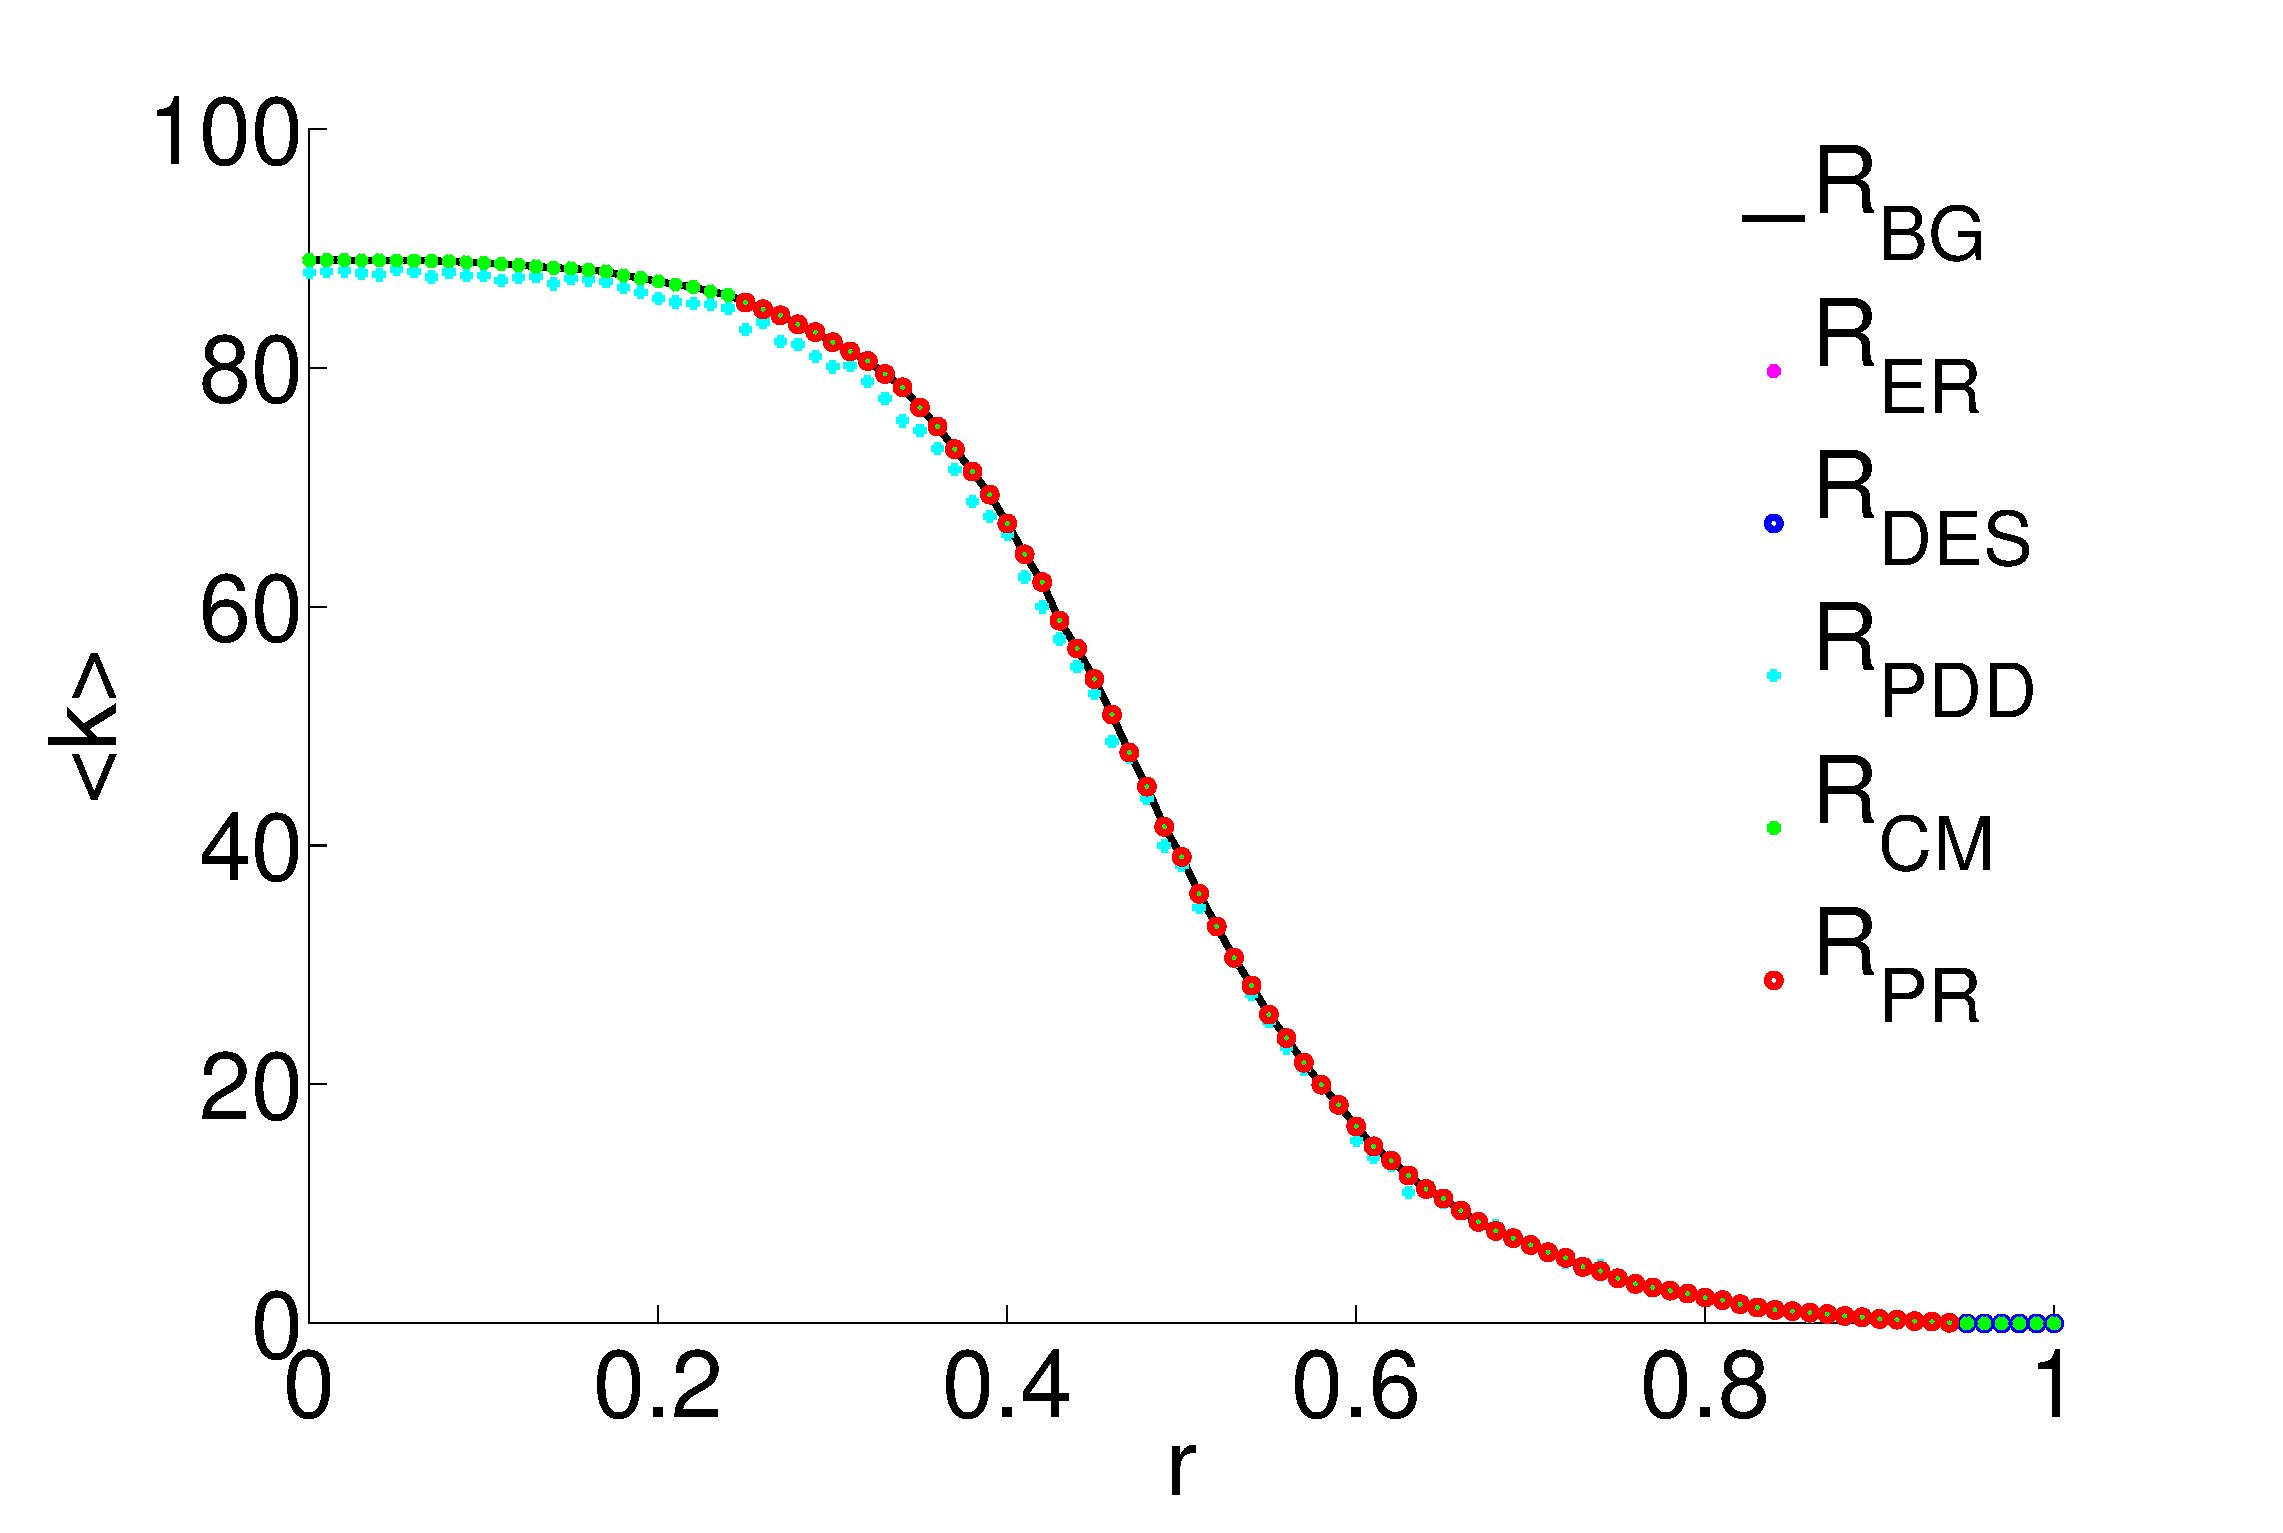
\includegraphics[width=0.45\textwidth, height=60mm]{Degree_Average_Fnc.eps} &

    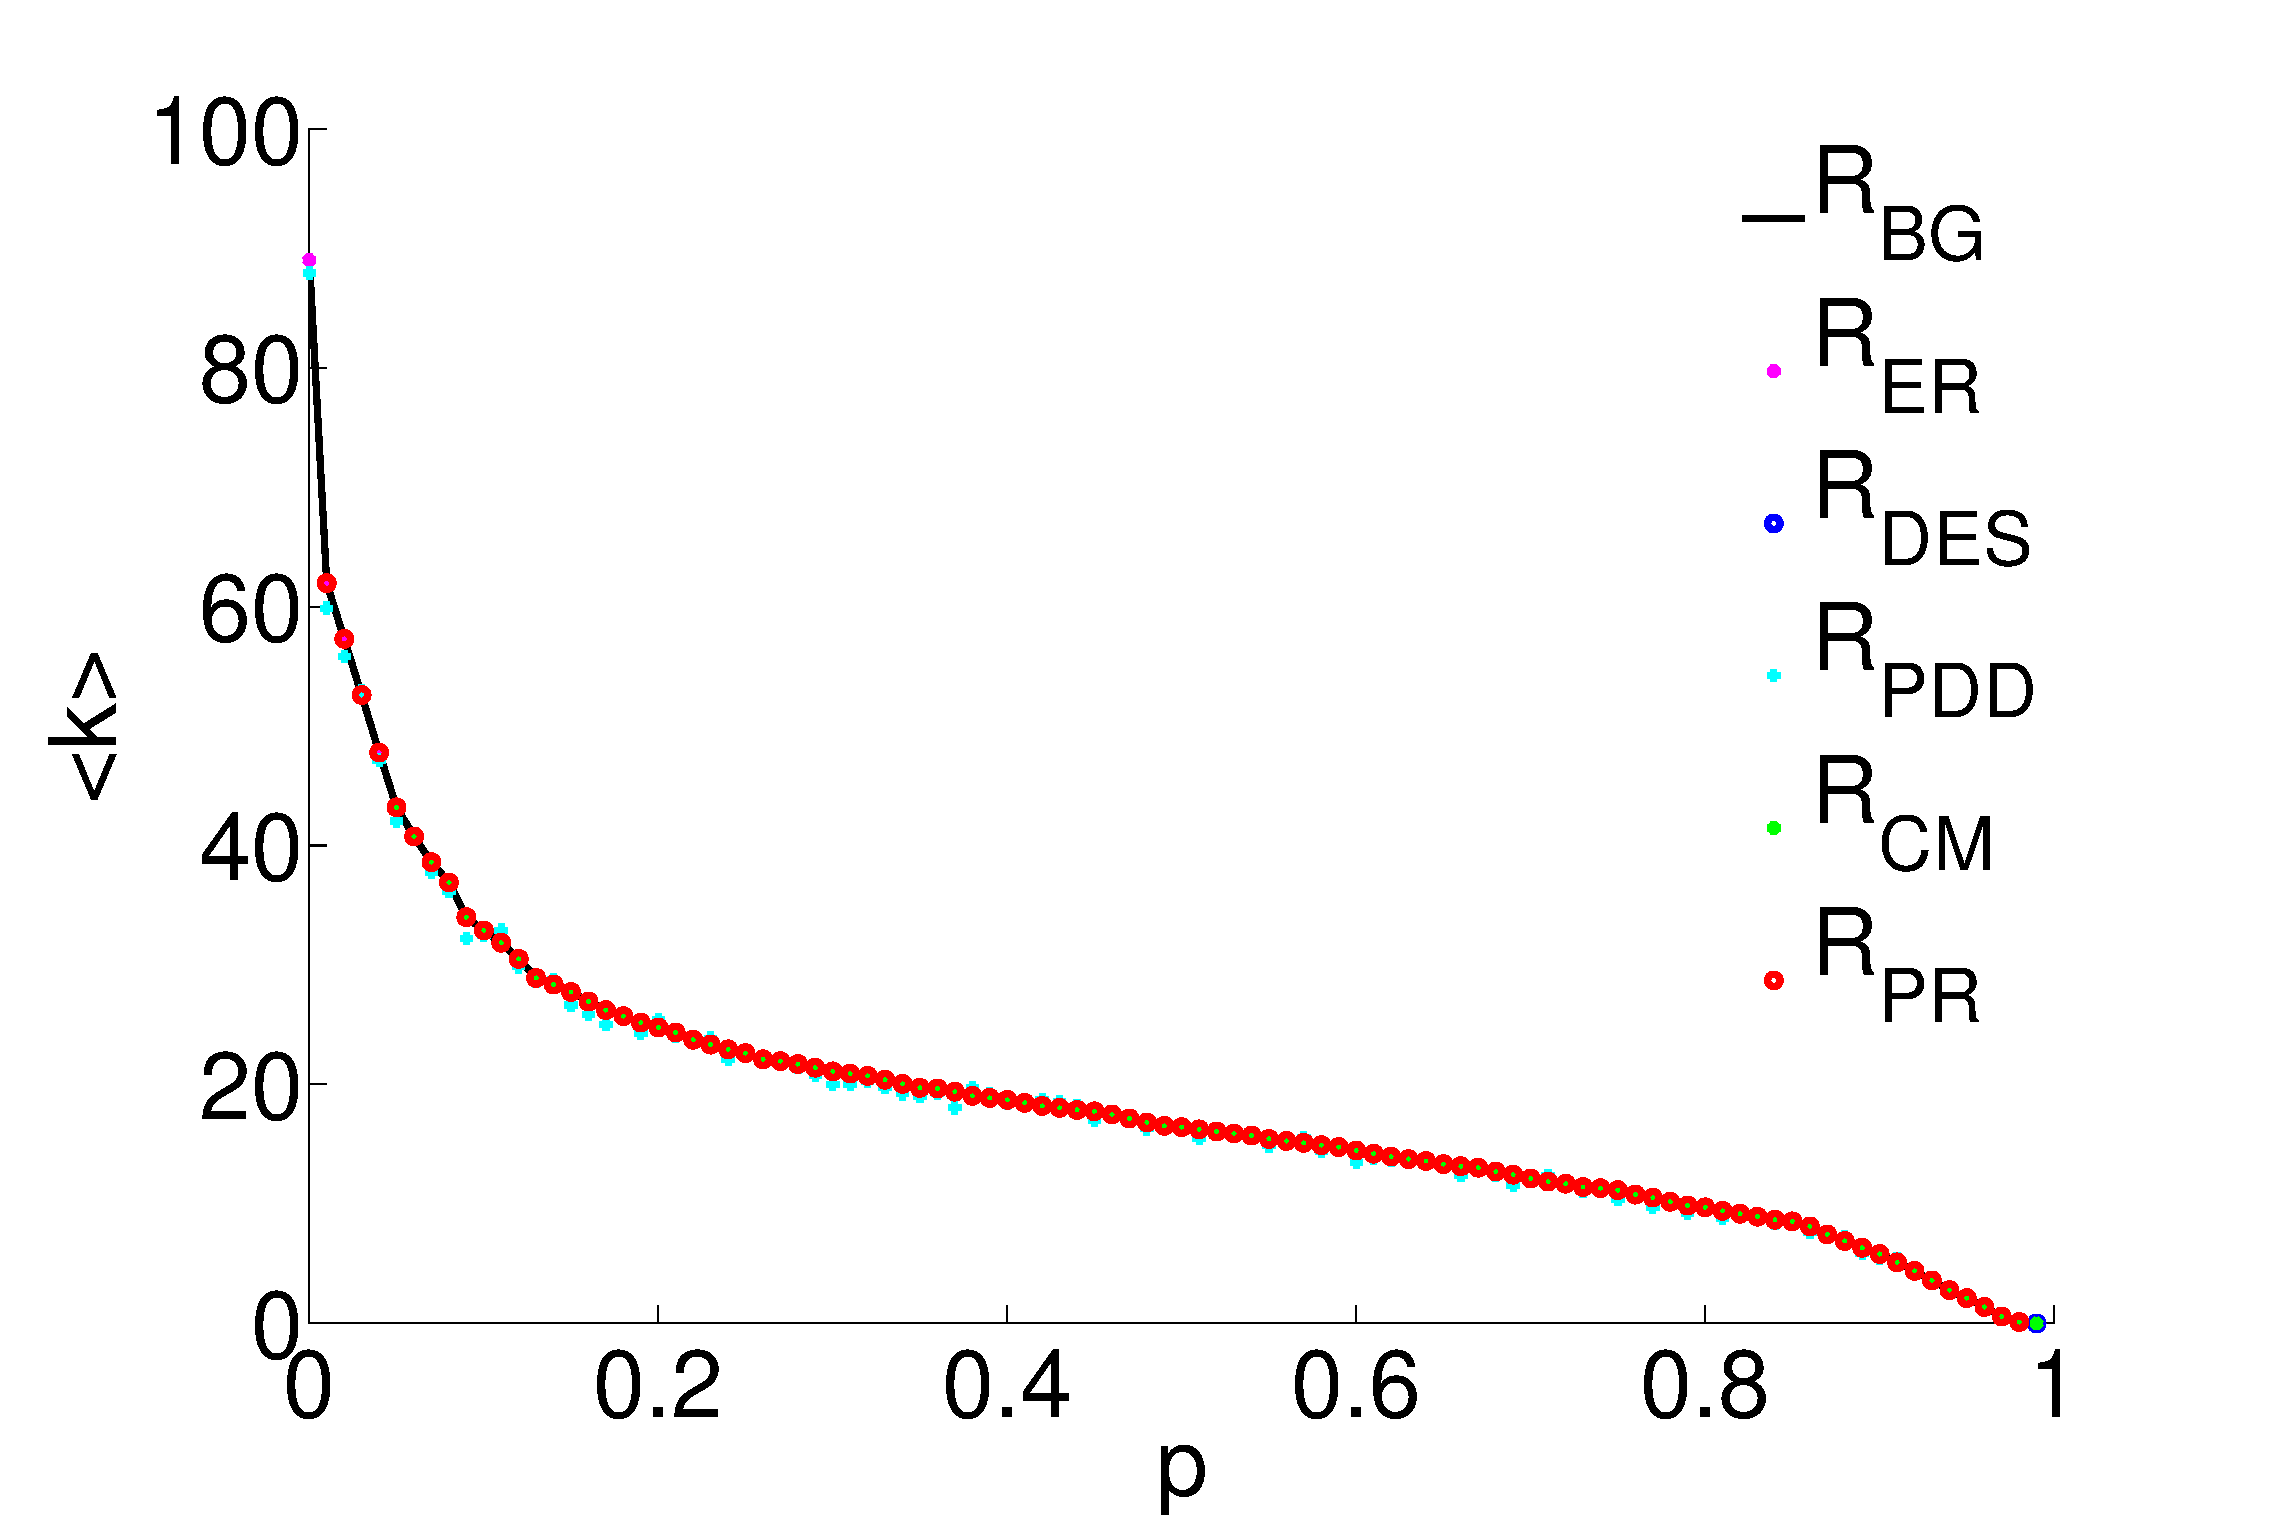
\includegraphics[width=0.45\textwidth, height=60mm]{Degree_Average_Stru.eps}\\

  \end{tabular}

 \label{figur}\caption{Average degrees of the original network and the randomized networks. Left: $R0$ corresponds to the graph of FCM (source is $A\_aal.txt$), right: $R0$ is that of ACM (source is $acp\_w.txt$). Successful $r$ ranges for randomization methods of FCM :  $r_{Ra}=[0,1]$ , $r_{Rd} = [0.25,1.00]$, $r_{Rg} = [0,1.00]$ , $r_{Rh} = [0,1.00]$ , $r_{Rk} = [0.08,0.94]$. Successful $p$ ranges of ACM : $p_{Ra}=[0,0.99]$, $p_{Rd}=[0.01 , 0.99]$, $p_{Rg}=[0, 0.99]$ , $p_{Rh}=[0.05 , 0.98]$. }

\end{figure}
%
Degree is one of the statistical tools to measure the centrality of network. The higher the average degree is, the more interaction the nodes in the graph have. 

Increasing threshold and probability values diminishes number of edges inverse sigmoidally. As long as the total node numbers, total edge numbers and networks density are all preserved while constructing the random graphs, the average degree remains the same. 

\subsection{Network Density}

The denstiy of a network (\textit{D}) is given by the following equation.

\begin{equation}
D = \frac{2L}{N(N-1)}
\end{equation}	

The formula above describes the density as the ratio between the number of total edges and maximum number of possible edges, ${N \choose 2} $. The density is a scaled version of average degree measure. 
	
\begin{figure}[htp]

  \centering

    \begin{tabular}{cc}

    % Requires \usepackage{graphicx}

    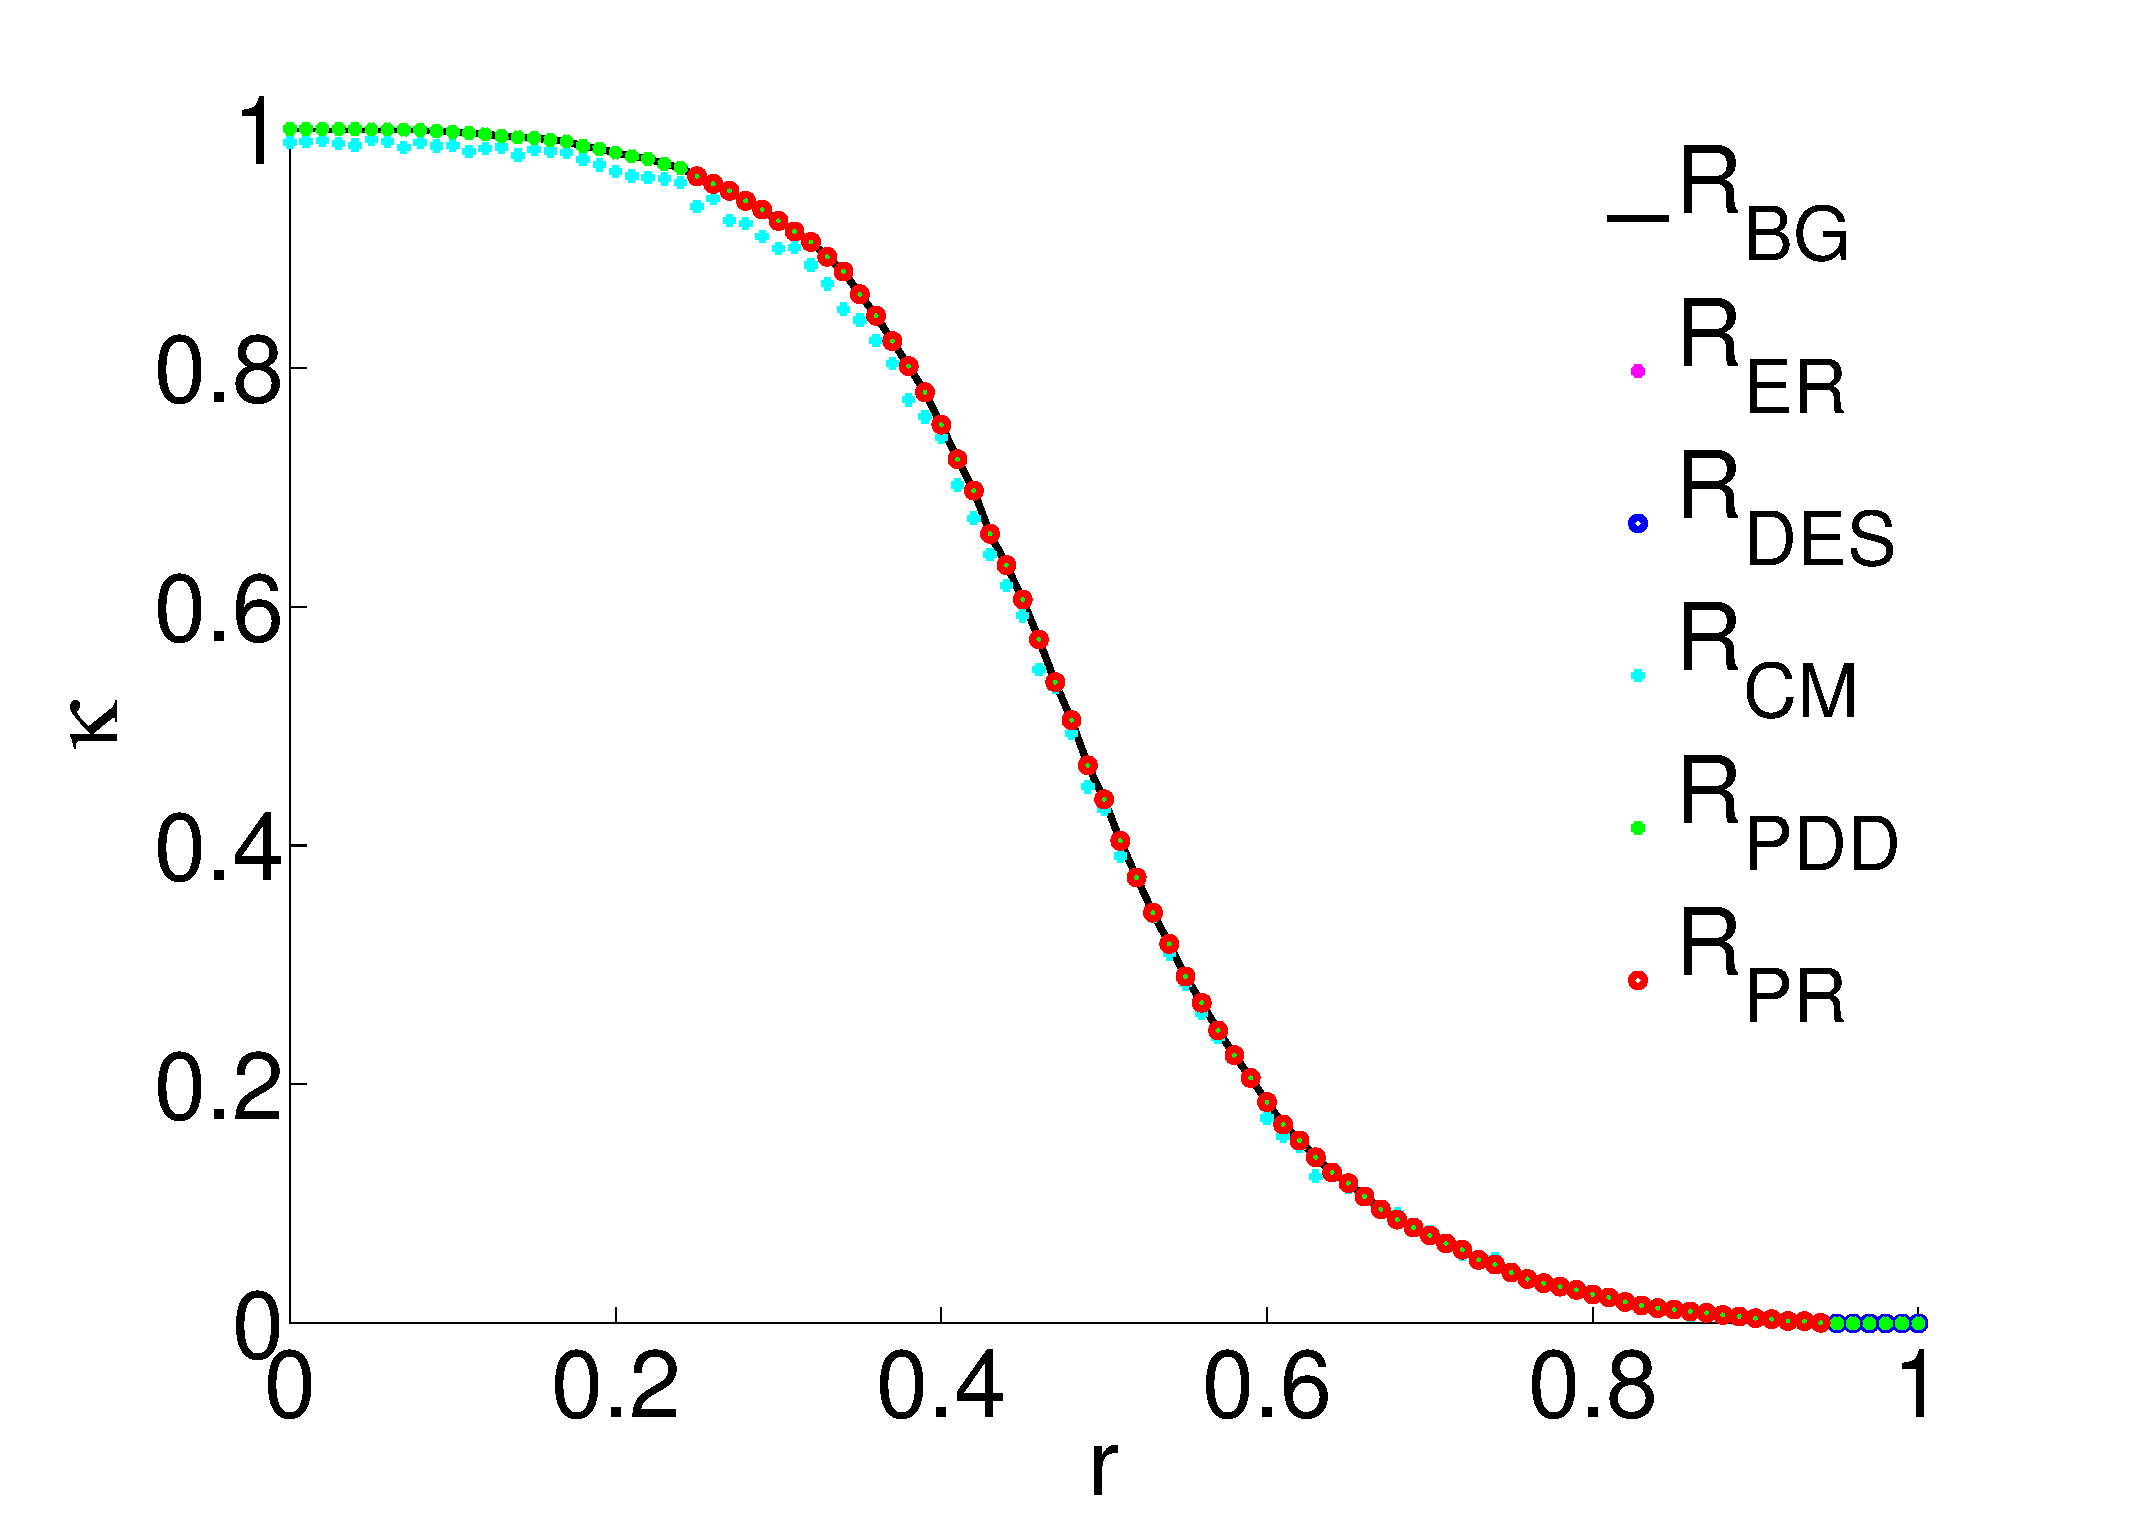
\includegraphics[width=0.45\textwidth, height=60mm]{Network_Density_Fnc.eps} &

    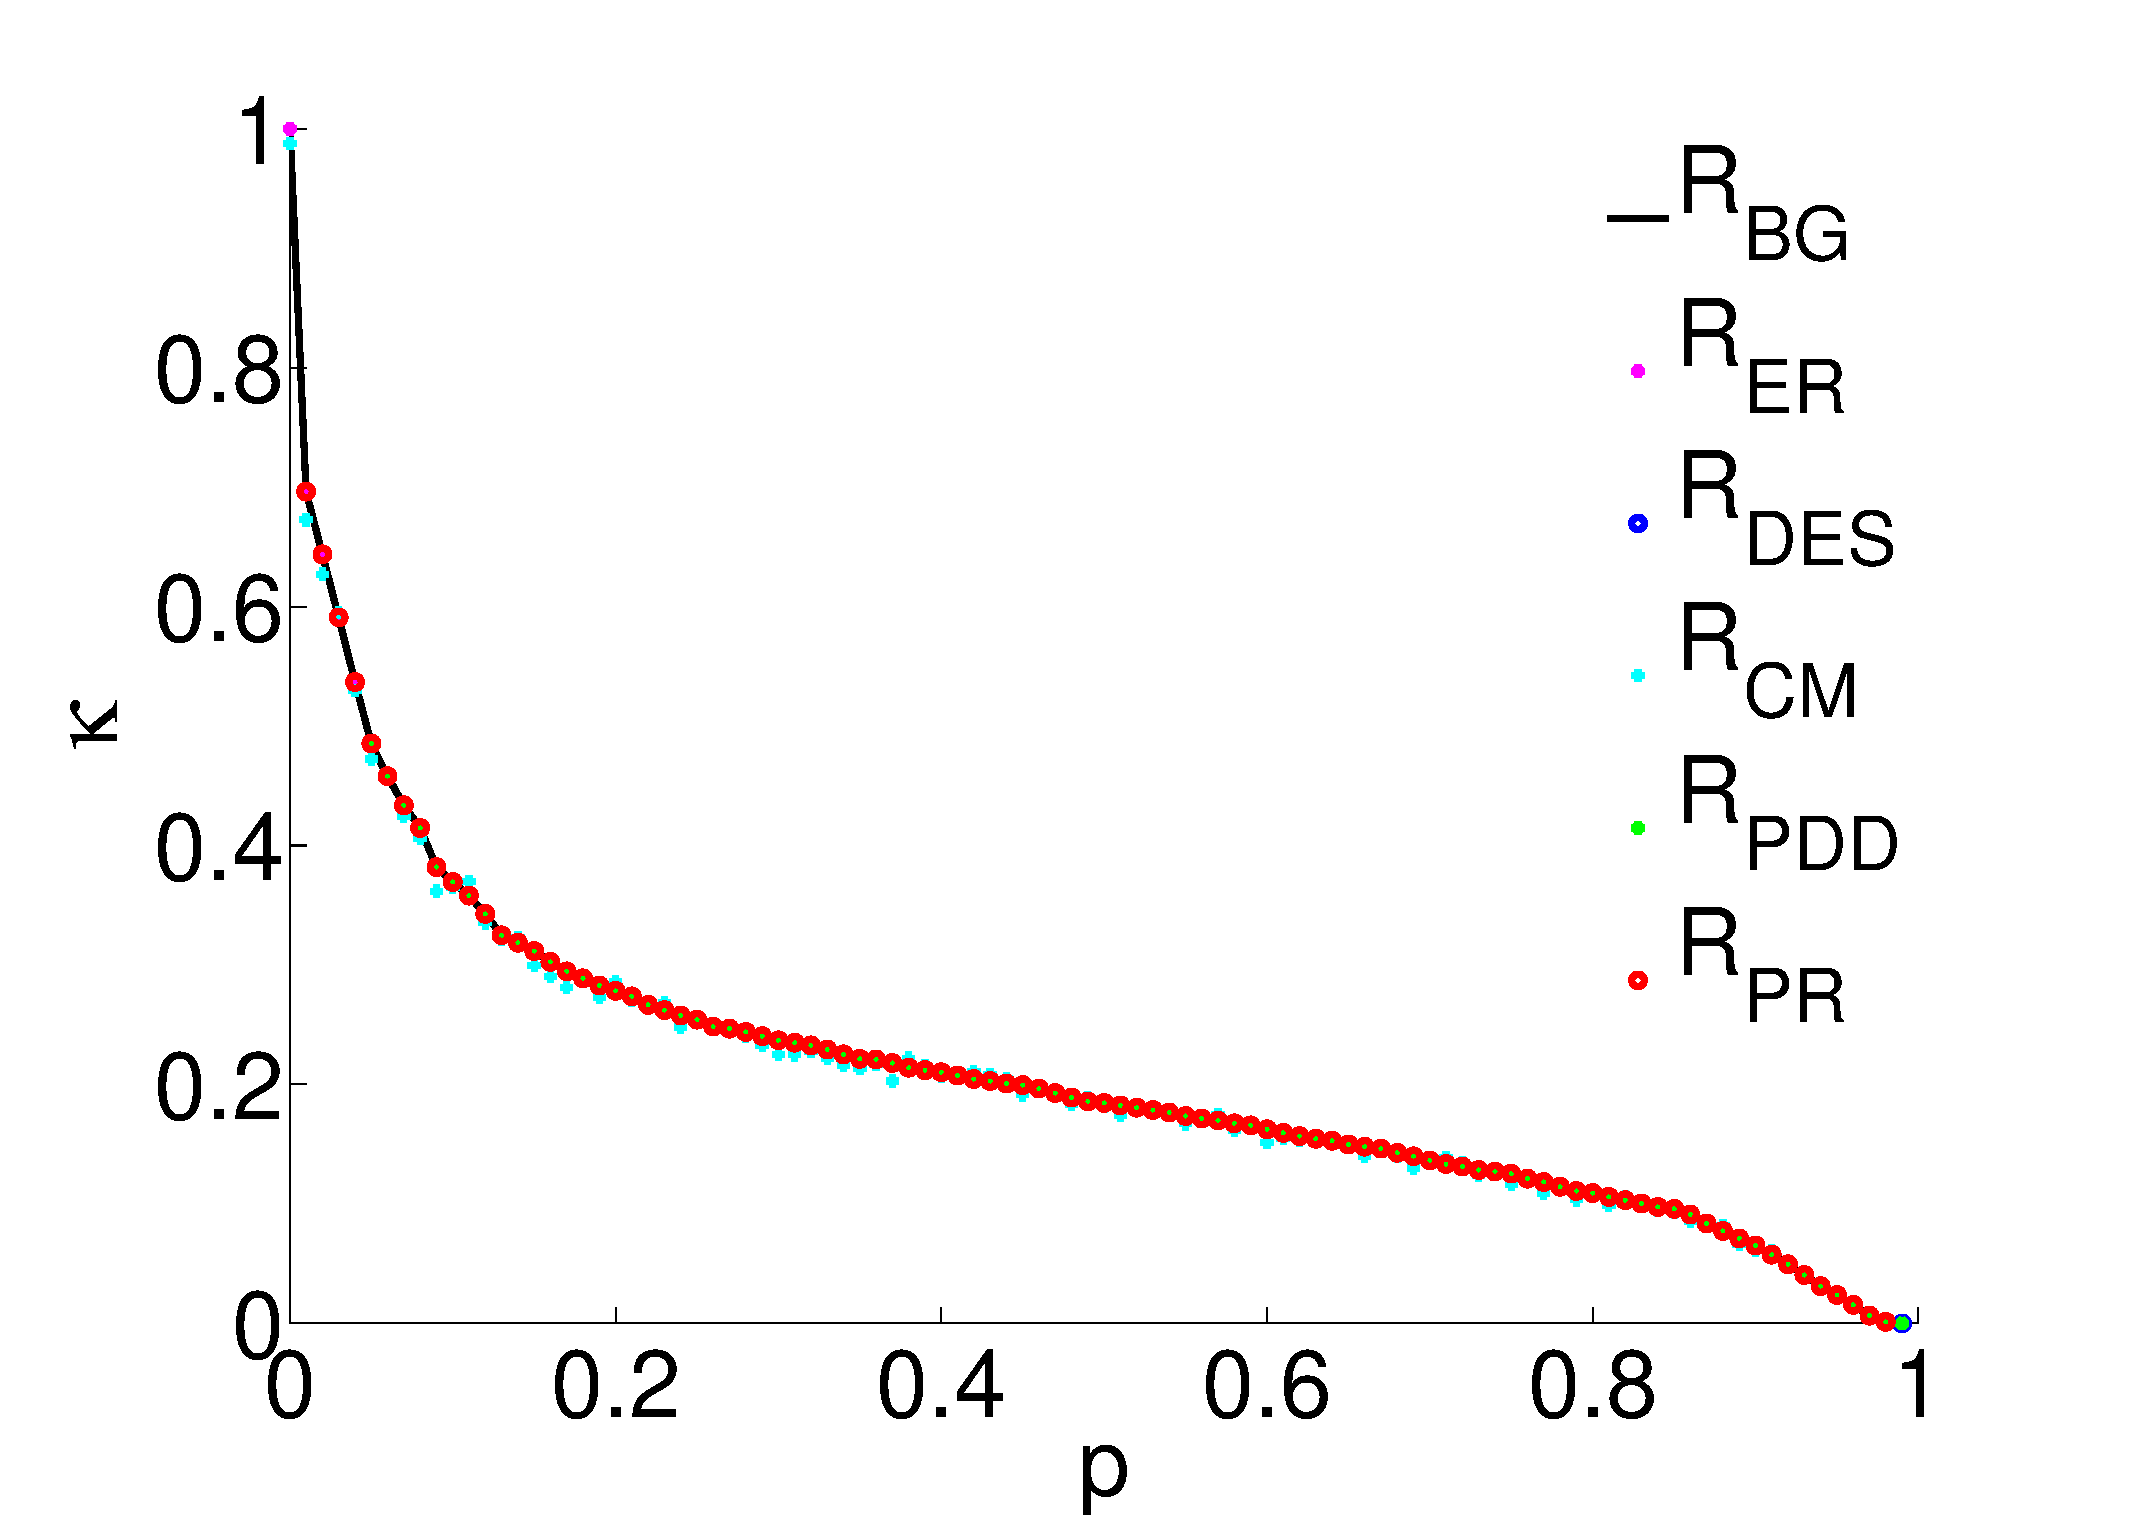
\includegraphics[width=0.45\textwidth, height=60mm]{Network_Density_Stru.eps}\\

  \end{tabular}

 \label{figur}\caption{Network density measure of test and random networks are similar to the Figure 1, except that the network density represents a probability value over all possible nodes, therefore it is lying between 0 and 1.}

\end{figure}

All the networks seem to be densely connected at lower $r$ and $p$ values. The FCM graphs reach zero network density faster than ACM graphs which stay almost constant for higher $p$.

 
\subsection{Average Clustering Coefficient}

The average clustering coefficient (\textit{C}) of network is calculated through the clustering coefficients of single nodes ($C_i$):

\begin{equation}
C = \frac{1}{n} \sum\limits_{i\epsilon N}C_i = \frac{1}{n}\sum\limits_{i\epsilon N} \frac{2t_i}{k_i(k_i -1)}
\end{equation} 

where $t_i$ is the number of triangles (triplets) around node $i$, $k_i$ is the degree (number of links connected to the node) of node $i$ (Watts and Strogatz, 1998). Clustering coefficient is a measure of segregation, it reveals how the single nodes in a graph cluster together.

\begin{figure}[htp]

  \centering

    \begin{tabular}{cc}

    % Requires \usepackage{graphicx}

    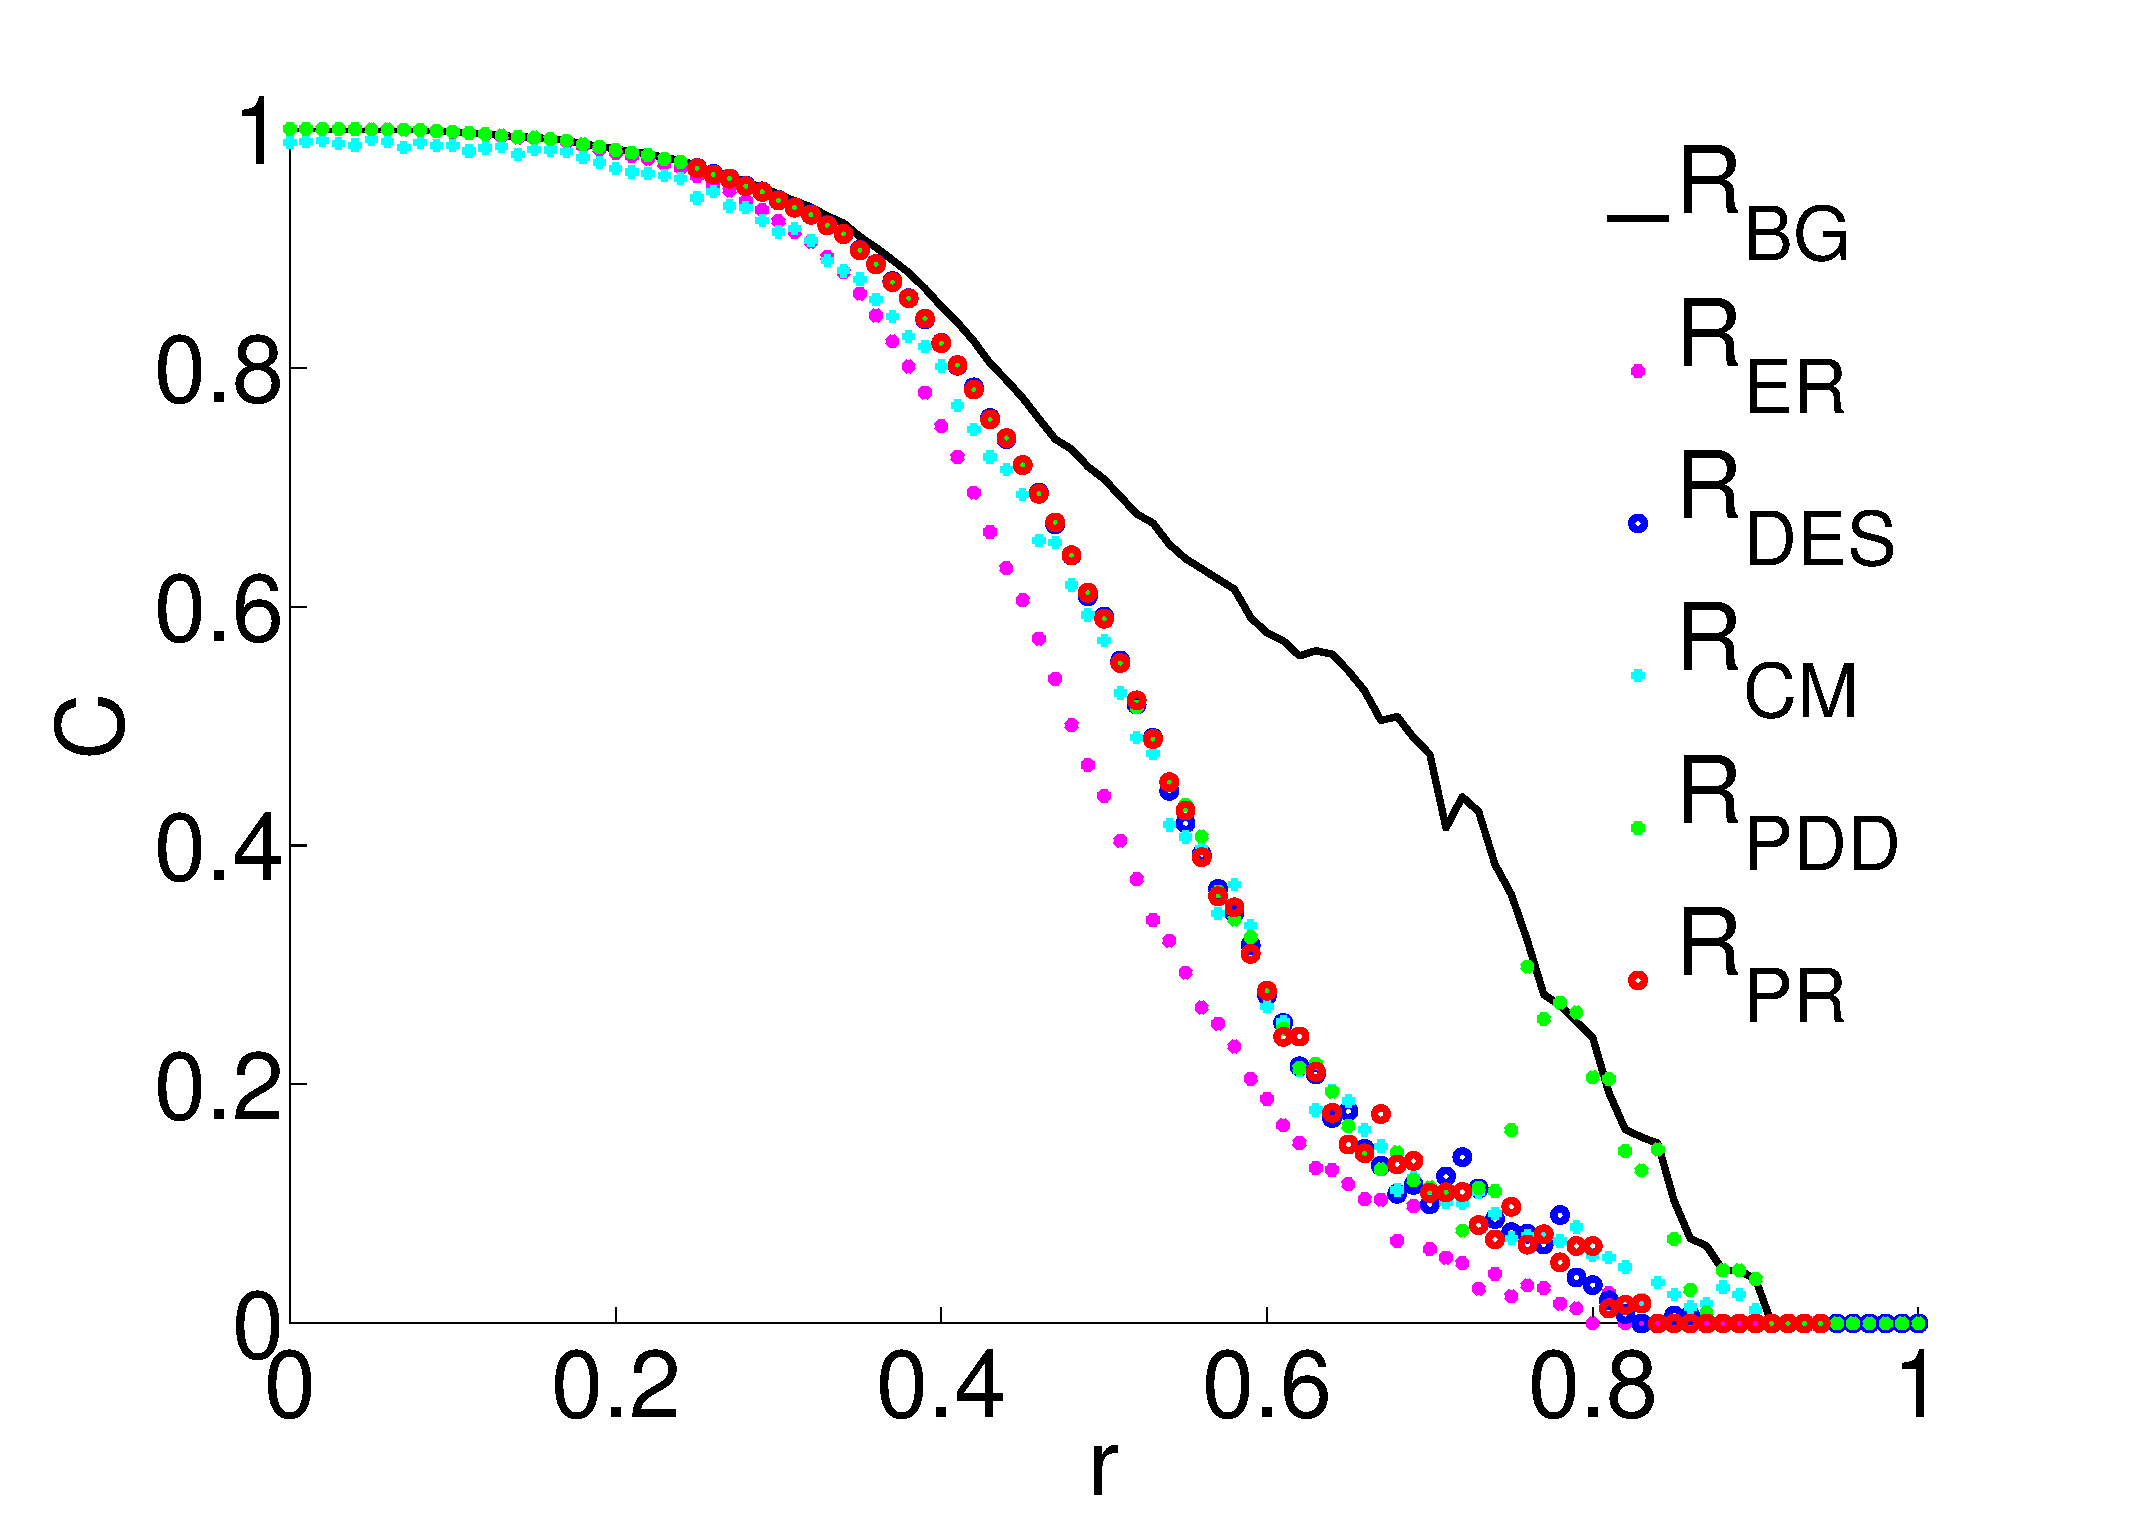
\includegraphics[width=0.45\textwidth, height=60mm]{Clustering_Coefficient_Fnc.eps} &

    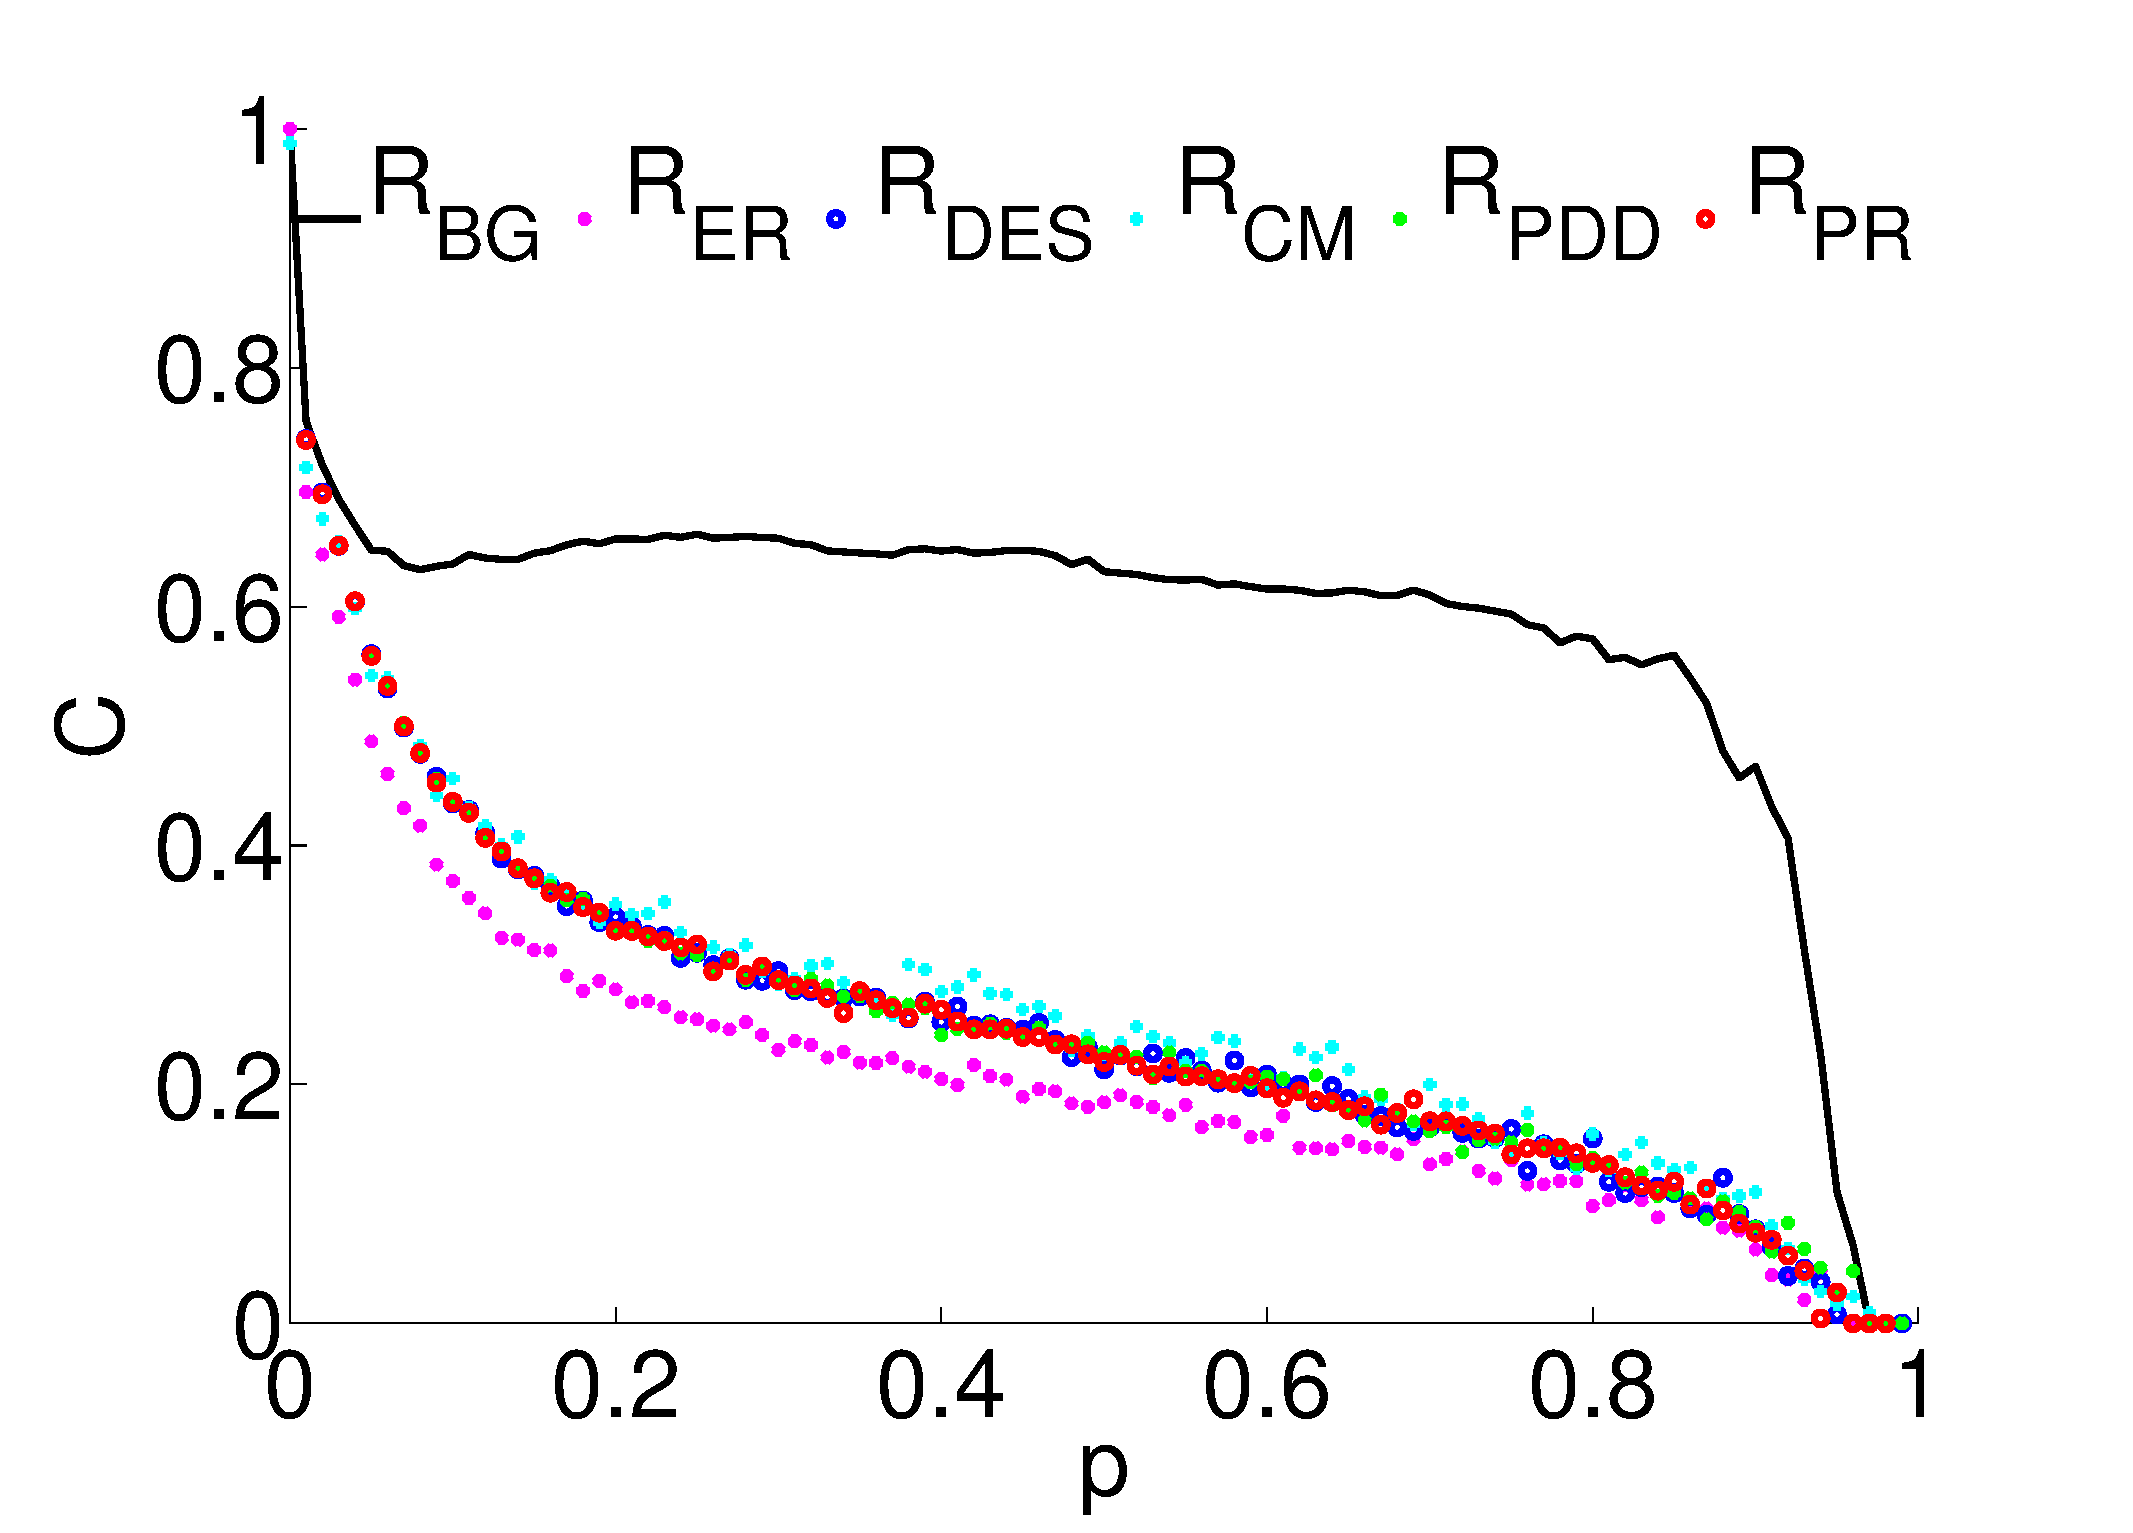
\includegraphics[width=0.45\textwidth, height=60mm]{Clustering_Coefficient_Stru.eps}\\

  \end{tabular}

 \label{figur}\caption{Average clustering coefficient of the test networks and the randomized networks. All the randomization methods besides $Rk$ lead random graphs having slightly lower average clustering coefficients ($cc$) than that of $R0$. However, the method $Rk$ has almost the same $cc$ as $R0$ for both FCM and ACM.}

\end{figure}


Clustering coefficient is formulated as the ratio of $t_i$ over all possible edges of the node $i$; ${k_i \choose 2} $. Since this resembles the probability, all $cc$ values are between 0 and 1. Figure 3 shows that at lower threshold, the nodes tend to cluster more due to higher number of existing edges. The empirically obtained original network has the highest $cc$ compared to random graphs, and has a good agreement with $Rk$ method. The real brain functional and structural networks seem to be higher clustered than our randomized networks in general.	


\subsection{Connected Components}

The connected components of an indirected graph indicates the number of subgraphs in overall network. Subgraph can be imagined as a connected group of vertices which has globally no connection to any other subgraph. In order to visualize subgraphs algebraically, let us define number of edges $L$ of graph $G$ in terms of three subgraphs of $G$: $L_G = L_{G_1}\cup L_{G_2}\cup L_{G_3}$. 

\begin{figure}[htp]

  \centering

    \begin{tabular}{cc}

    % Requires \usepackage{graphicx}

    \includegraphics[width=0.45\textwidth, height=60mm]{Connected_Components_Average_Fnc.eps} &

    \includegraphics[width=0.45\textwidth, height=60mm]{Connected_Components_Average_Stru.eps}\\

  \end{tabular}

 \label{figur}\caption{Number of connected components of the test networks and the randomized networks. The number of subgraphs remains to be for the threshold values $r<0.65$ in the FCM graphs and for the probability values $p<0.80$ in the ACM graphs.  }

\end{figure}


We can expect that the nodes are assumed to be well connected at lower $r$ and $p$, it is always possible to visit any node in the network through the edges, when started from any other node. That means subgraphs should begin to be constructed after a high $r$ and $p$ values.  

Figure 4 shows that, at higher $r$ and $p$ levels, the nodes become sparse as the network densities get lower in FCM and ACM graphs. When $r>0.95$ and $p=1.00$, we can imagine each node as a single subgraph, since none of the nodes is connected. 

\newpage

\subsection{Transitivity}
	Transitivity is a similar measure to the clustering coefficient, it is also a measure for the segregation in the network. The mean clustering coefficient is normalized individually for each node [RUB10]. The corresponding equation represents the transitivity of a network (Newman, 2003):
	
\begin{equation}
 T = \frac{\sum\limits_{i \epsilon N} 2 t_i}{\sum\limits_{i \epsilon N}k_i (k_i - 1)}
\end{equation}	

If a node has links to two other nodes, transitivity inquires whether those two other nodes are also connected to each other. Transitivity is defined only for the whole network rather than single nodes. 

\begin{figure}[htp]

  \centering

    \begin{tabular}{cc}

    % Requires \usepackage{graphicx}

    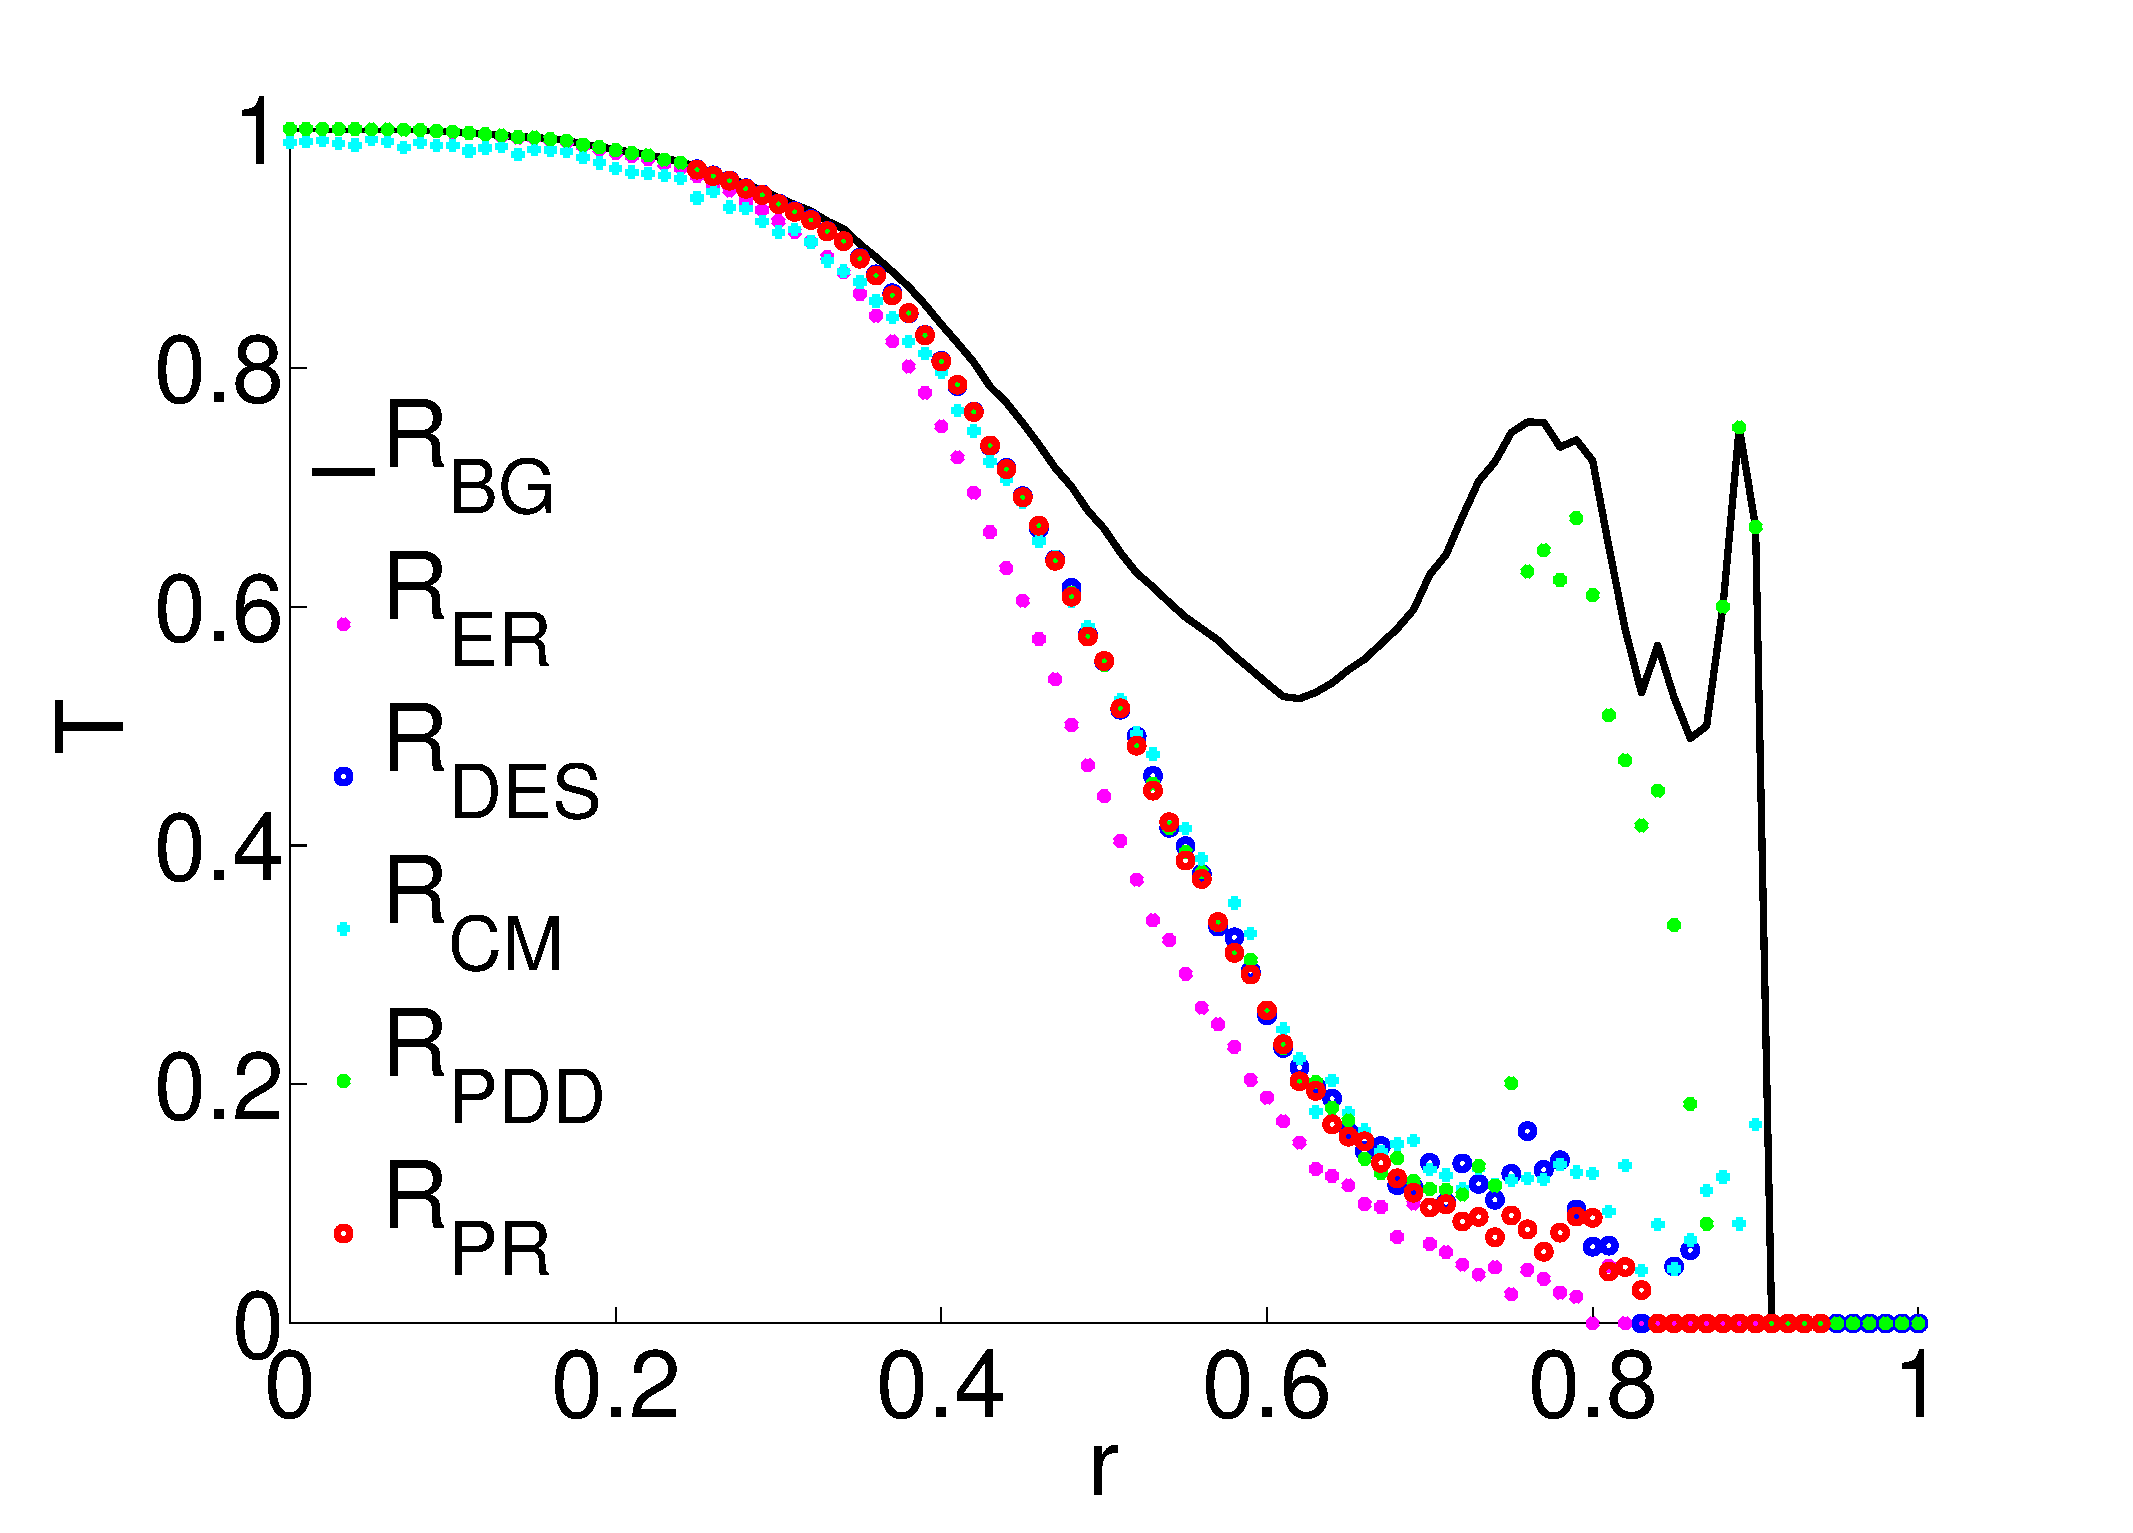
\includegraphics[width=0.45\textwidth, height=60mm]{Transitivity_Fnc.eps} &

    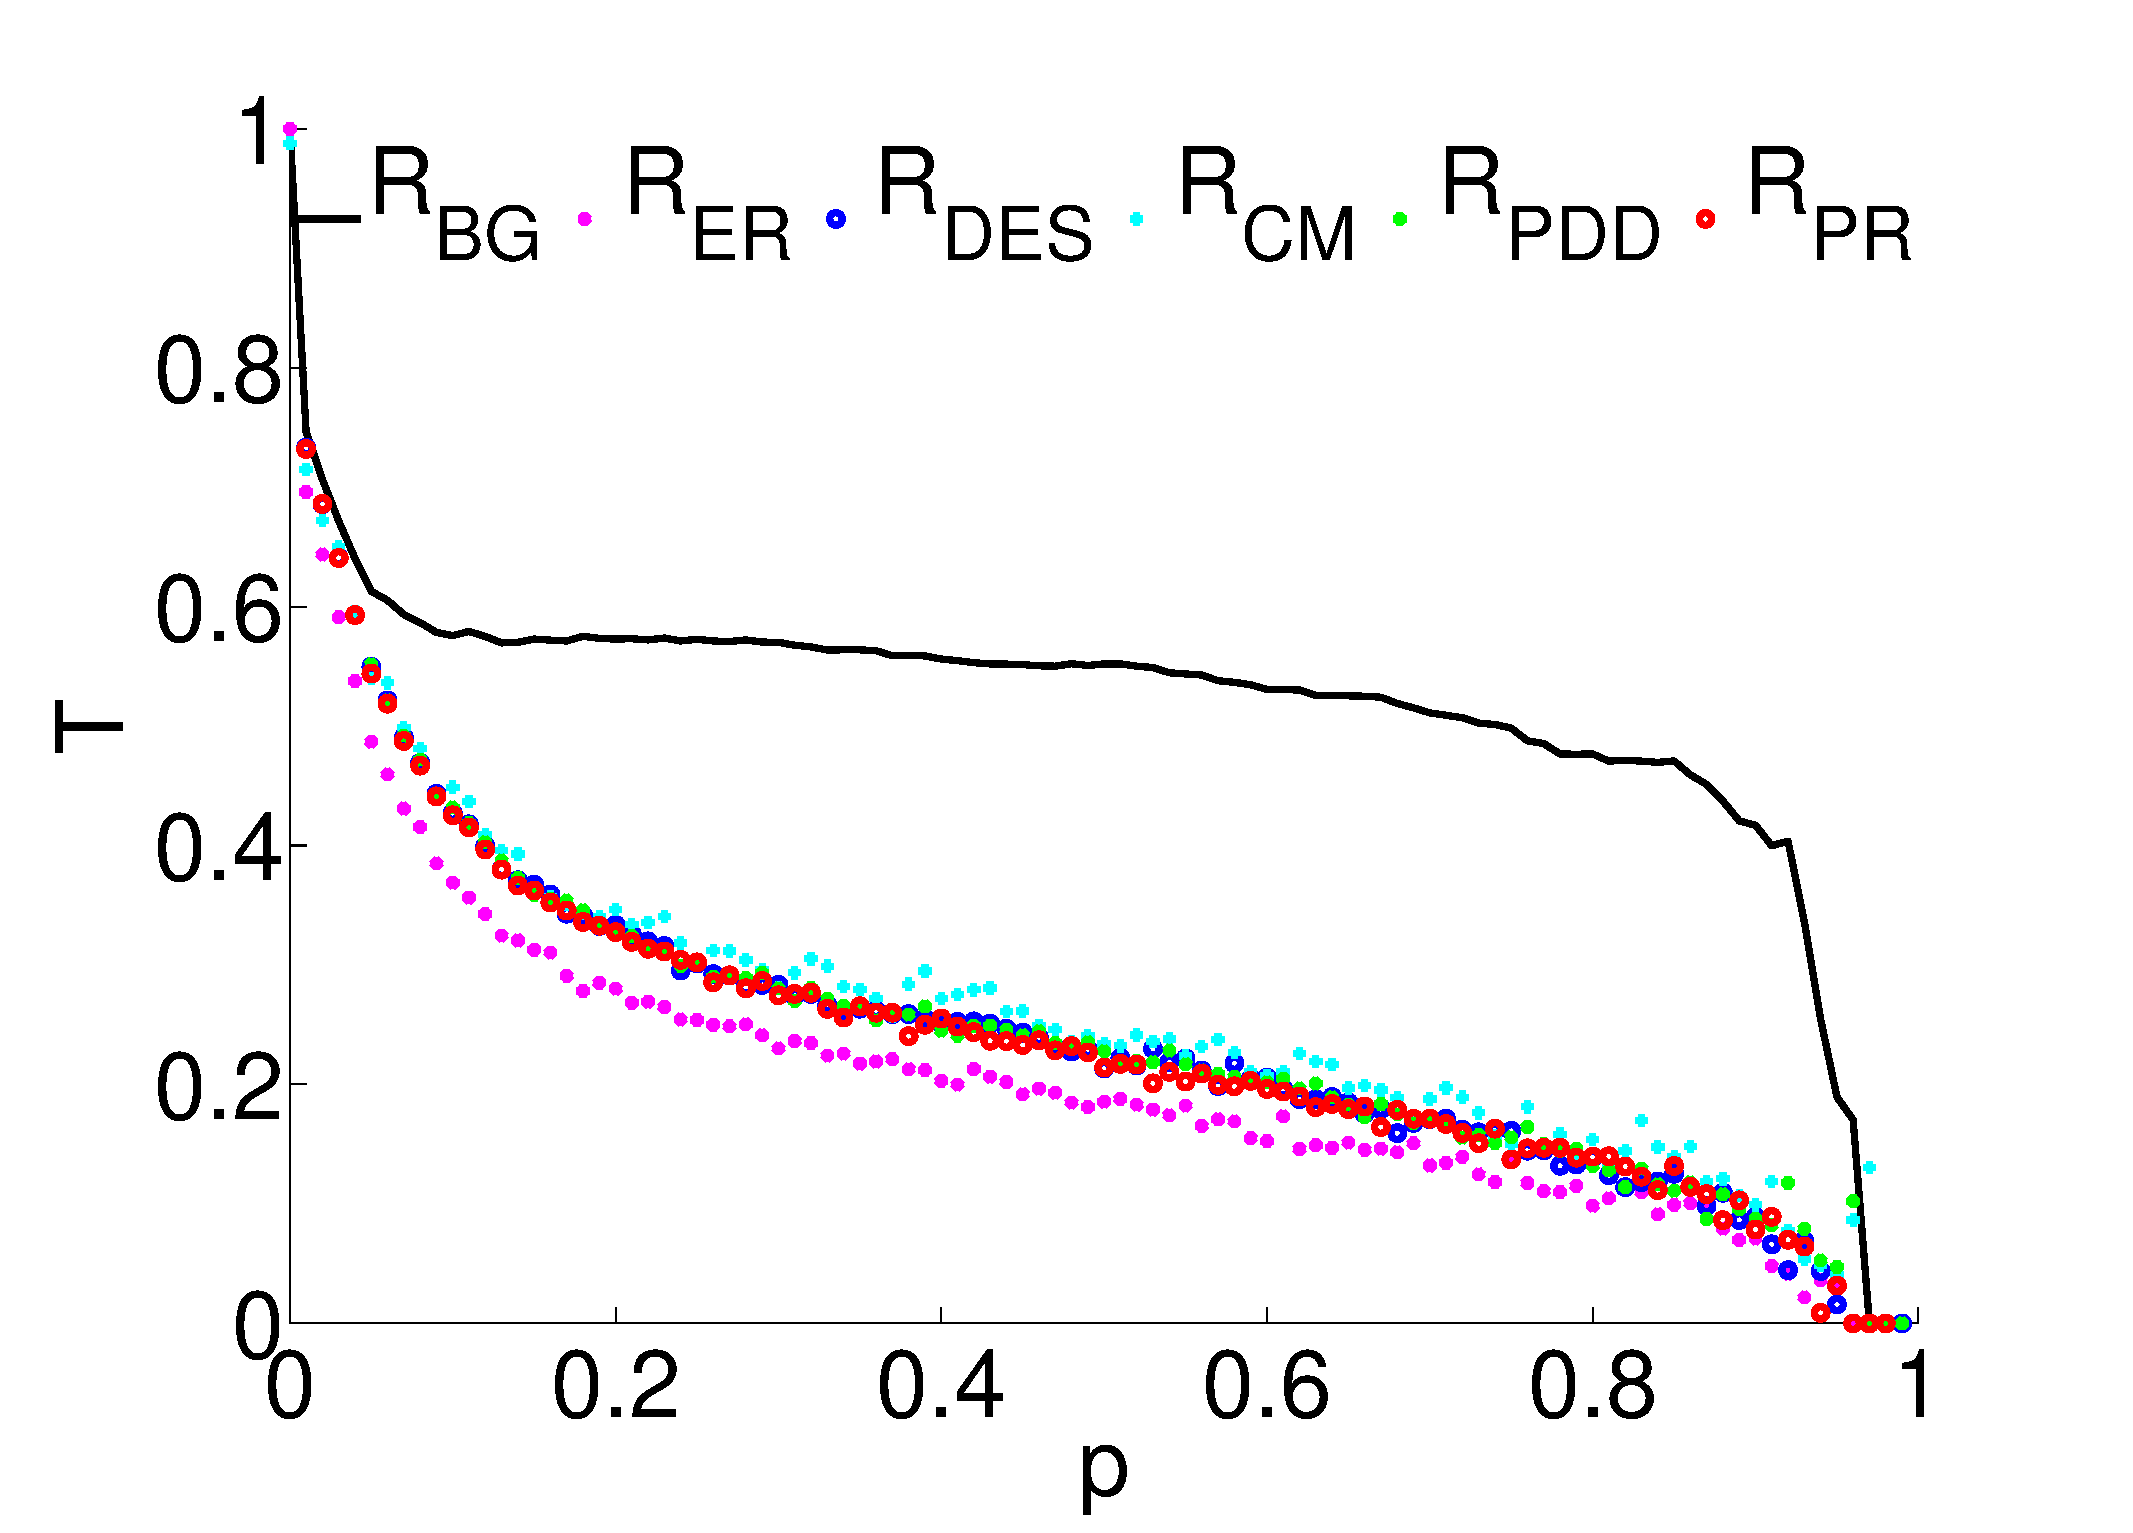
\includegraphics[width=0.45\textwidth, height=60mm]{Transitivity_Stru.eps}\\

  \end{tabular}

 \label{figur}\caption{Transitivity of the test networks and the randomized networks. The transitivity evolves as the clustering coefficient up to a threshold value. }

\end{figure}

In Figure 5, the transitivity of random graphs $Ra$, $Rd$, $Rg$ and $Rh$ seems to differ highly from that of the test network $R0$ for both FCM and ACM. The transitivity of the random graph $Rk$ tends to match the best with that of $R0$. The method $Rk$ swaps the existing double edges in $R0$, as well as keeping degree distribution the same. We already expect that $Rk$ graph is very similar to $R0$, it is expected that the network measures of $Rk$ are in well agreement with that of $R0$.

Transitivity is one of severe shortcomings that real world networks and random networks strongly differ [NEW10]. Transitivity equation resembles the clustering coefficient, however transitivity becomes more sensitive with the changing number of subgraphs (Figure 3, 4, 5). The higher the number of average connected components in the graph is, the more the transitivity measure is distinguishable than clustering coefficient. 
   
\newpage
\subsection{Shortest Pathway}
Shortest pathway is a measure of integration in the network, opposite to the segregation measures. It corresponds to the shortest path length between two nodes in an unweighted graph.  

\begin{equation}
d_{ij} = \sum\limits_{a_{uv} \epsilon g_{i\leftrightarrow j} } a_{uv}
\end{equation}
where $g_{i\leftrightarrow j}$ is the shortest path between nodes $i$ and $j$. $d_{ij}$ is assumed to be $\infty$ for disconnected pairs.

\begin{figure}[htp]

  \centering

    \begin{tabular}{cc}

    % Requires \usepackage{graphicx}

    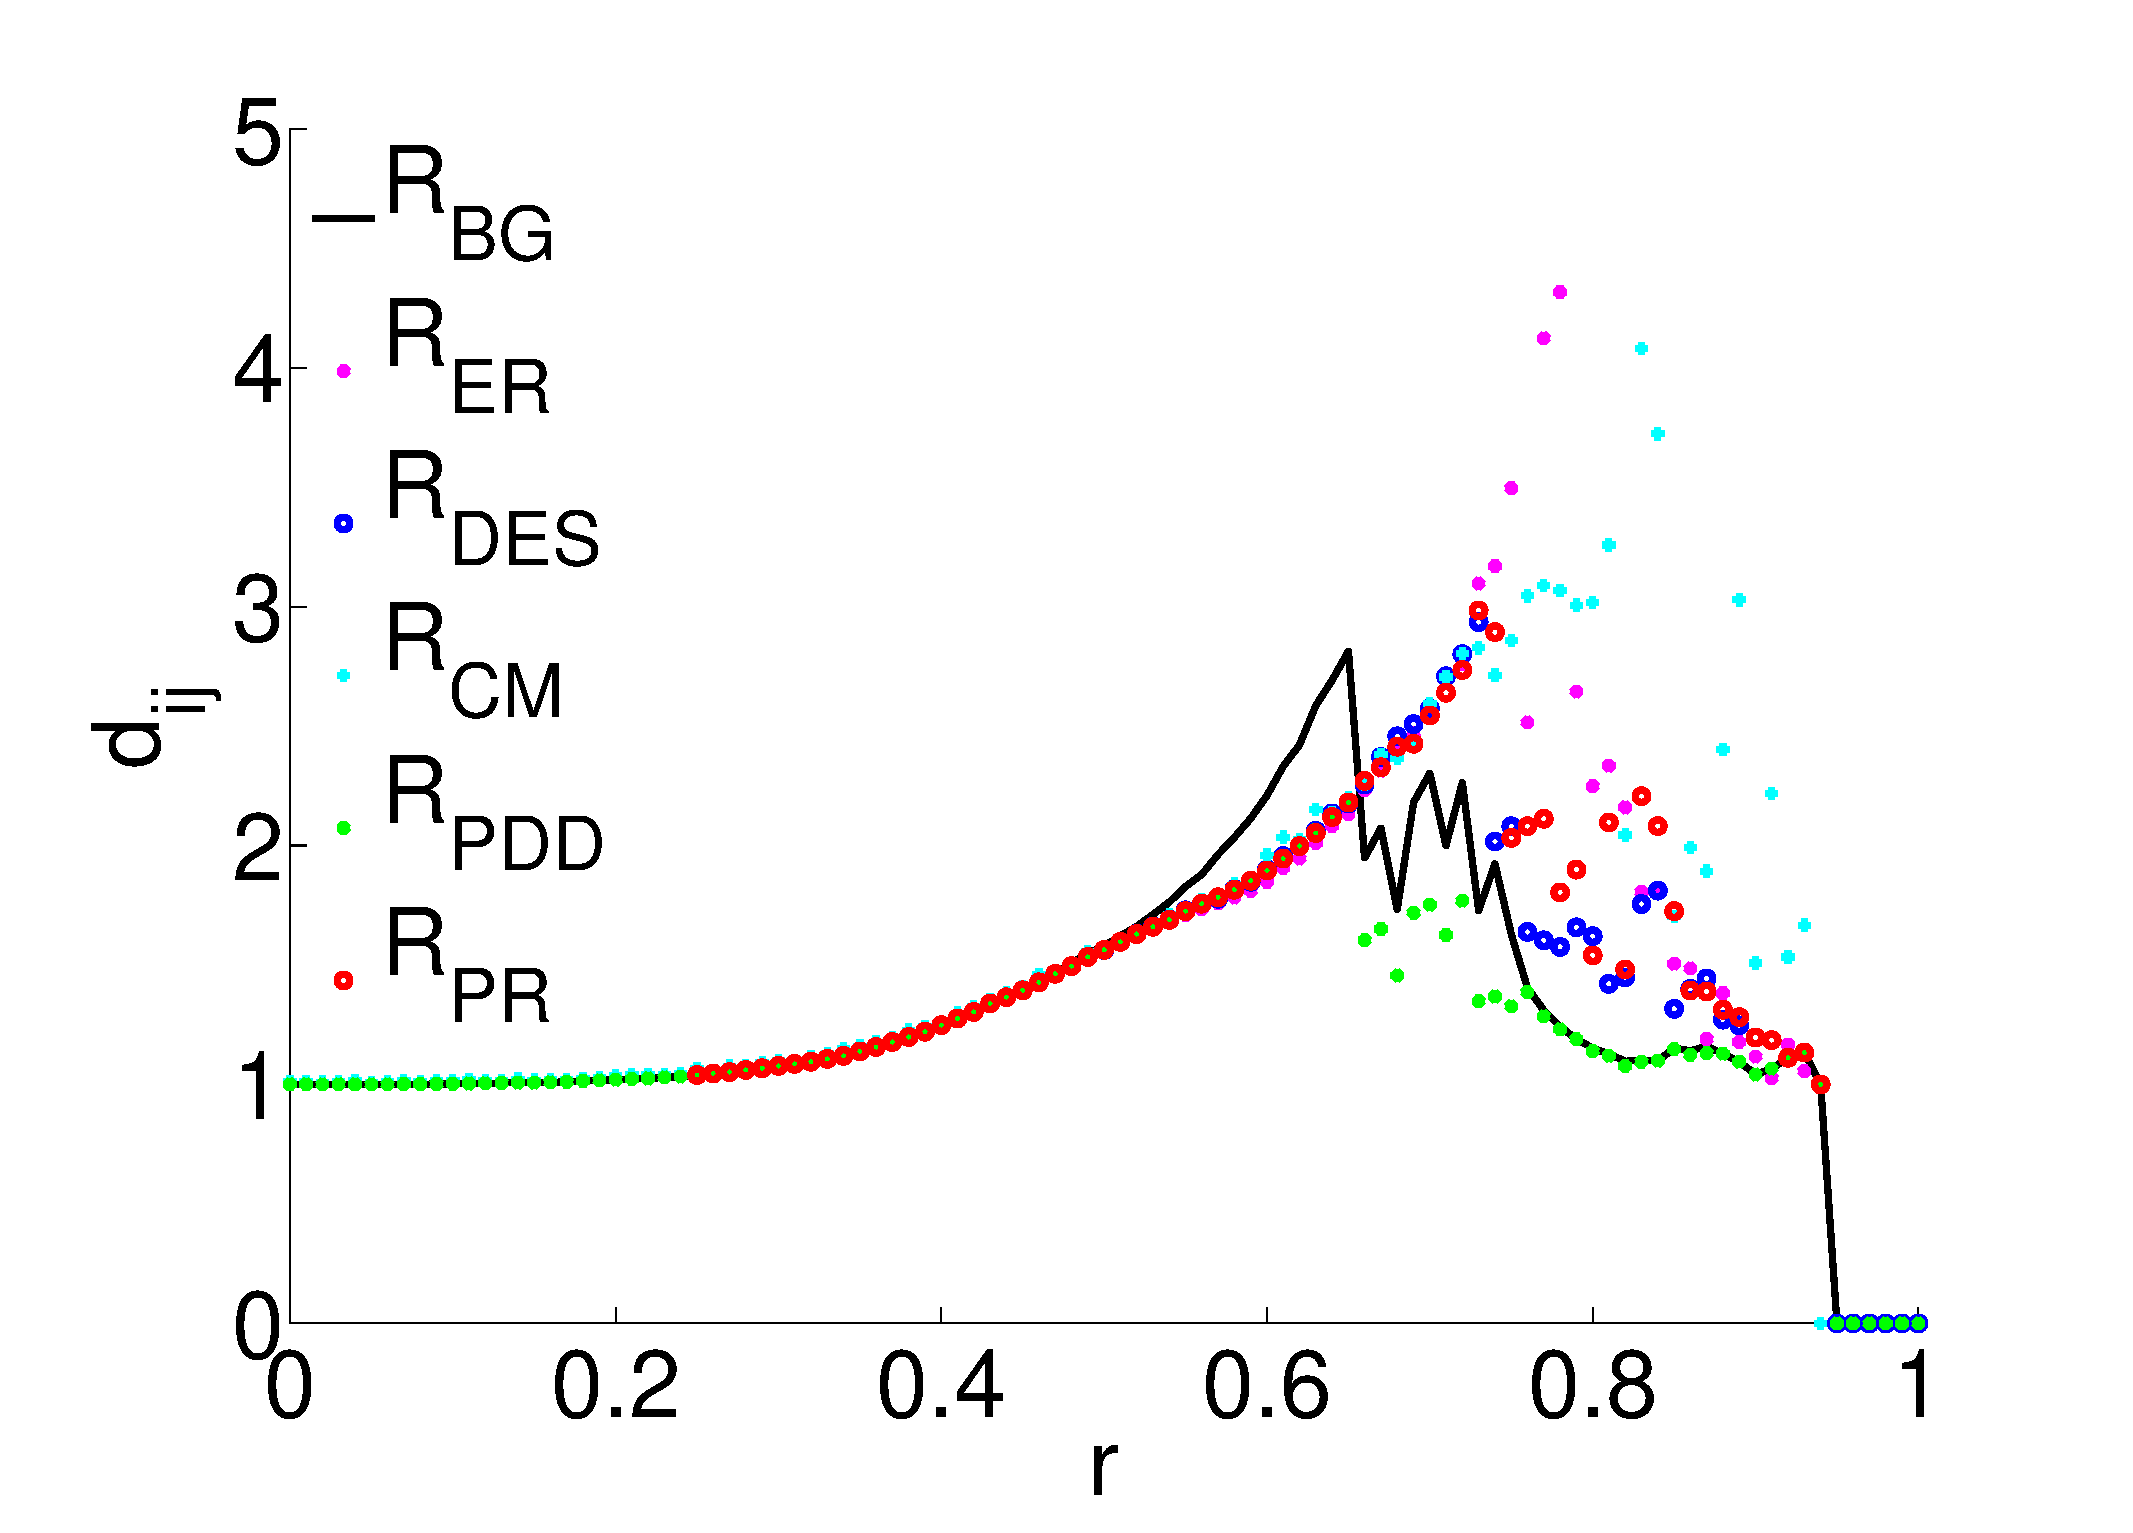
\includegraphics[width=0.45\textwidth, height=60mm]{Shortest_Pathway_Fnc.eps} &

    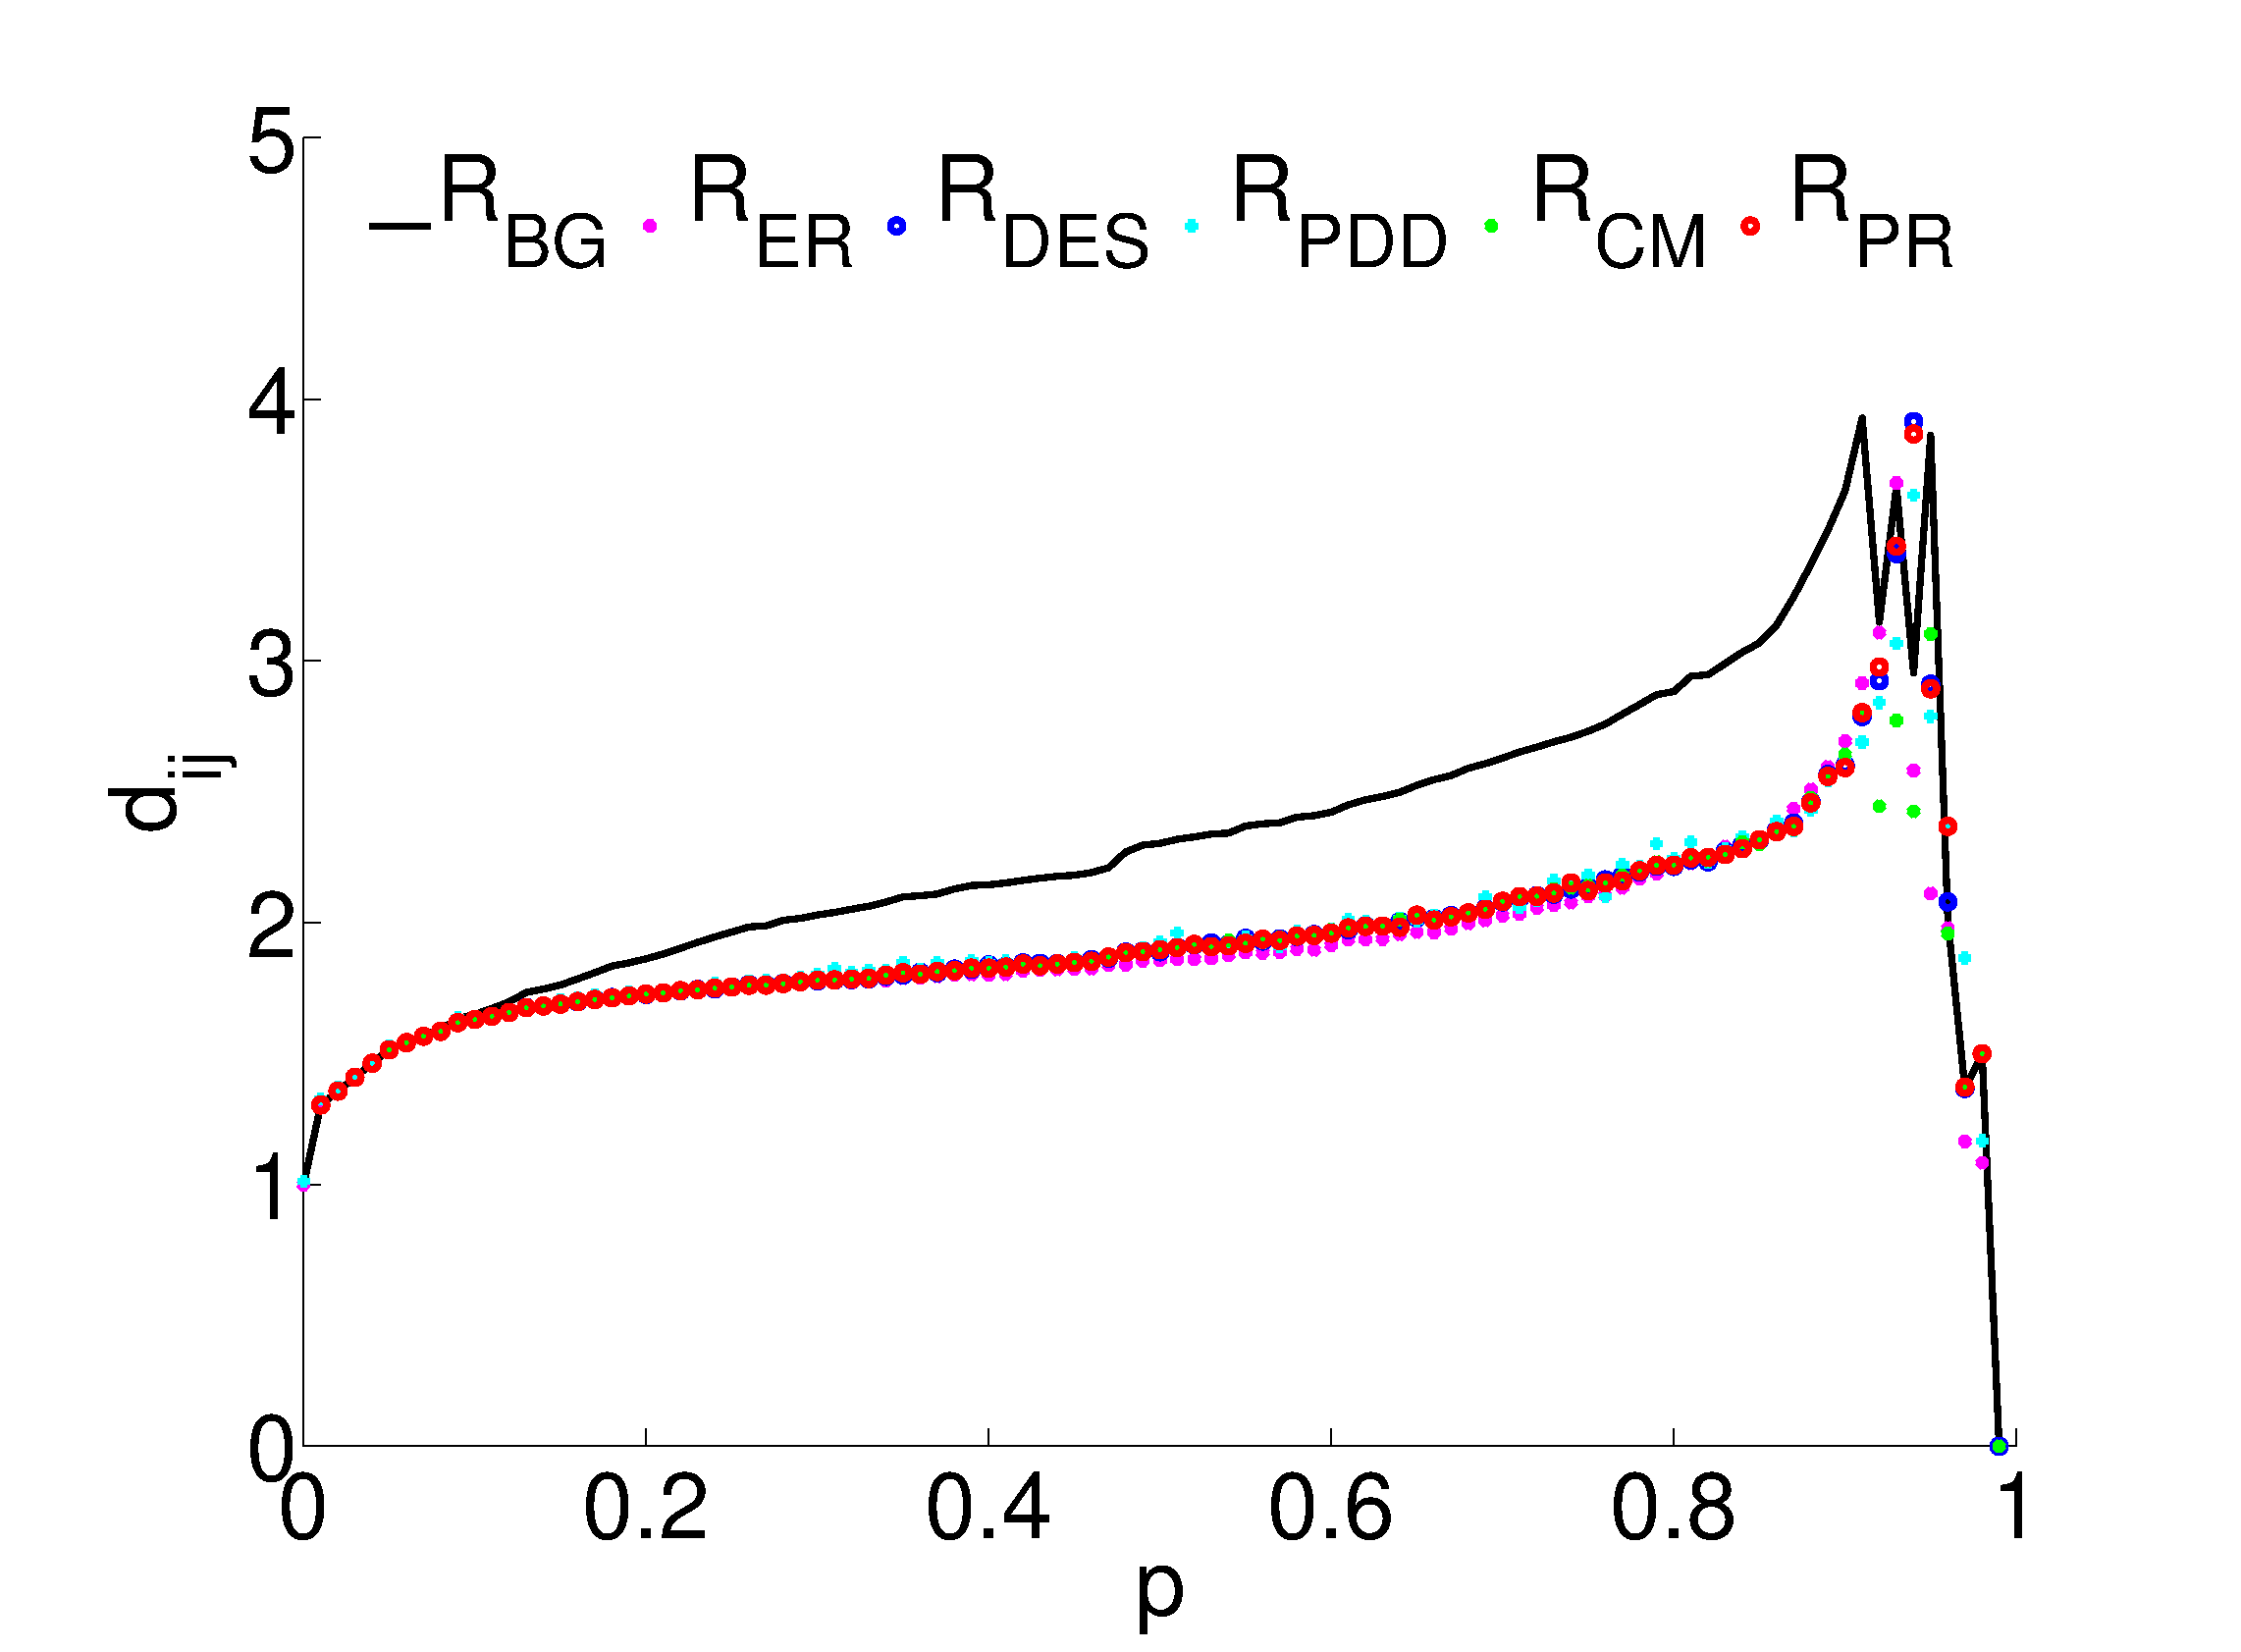
\includegraphics[width=0.45\textwidth, height=60mm]{Shortest_Pathway_Stru.eps}\\

  \end{tabular}

 \label{figur}\caption{Shortest pathway of the original networks and random graphs. }

\end{figure}

The $R0$ network of FCM seems to be less segregated than the randomized networks while $r$ lies between $[0.65,0.95]$. This is the threshold value at which the $R0$ network of FCM begins to get multiple components. The $R0$ network of ACM tends to be more segregated than random networks except for $Rk$ method. The graph constructed with the method $Rk$ seems to be the most segregated at all for ACM. Whenever all the nodes get sparse in both FCM and ACM networks, the shortest pathway is represented as 0. 
%
\subsection{Global Efficiency}
The global efficiency is measured as the average of the inverse shortest pathway (Latora and Marchiori, 2001);

\begin{equation}
E = \frac{1}{n}\sum\limits_{i \epsilon N} E_i = \frac{1}{n}\sum\limits_{i \epsilon N} \frac{\sum\limits_{j \epsilon N, j\neq i}d_{ij}^{-1}}{n-1 }
\end{equation}

where $E_i$ is the global efficiency of node, $d_{ij}$ is the shortest pathway between nodes $i$ and $j$. As seen from the equation, global efficiency becomes larger with smaller shortest pathways between nodes. The global efficiency is a measure of the integration in the network. It reveals the strength of connections in a network. Global efficiency measures the ability of a network to transmit information at the global level (Latora and Marchiori, 2001, 2003).

\begin{figure}[htp]

  \centering

    \begin{tabular}{cc}

    % Requires \usepackage{graphicx}

    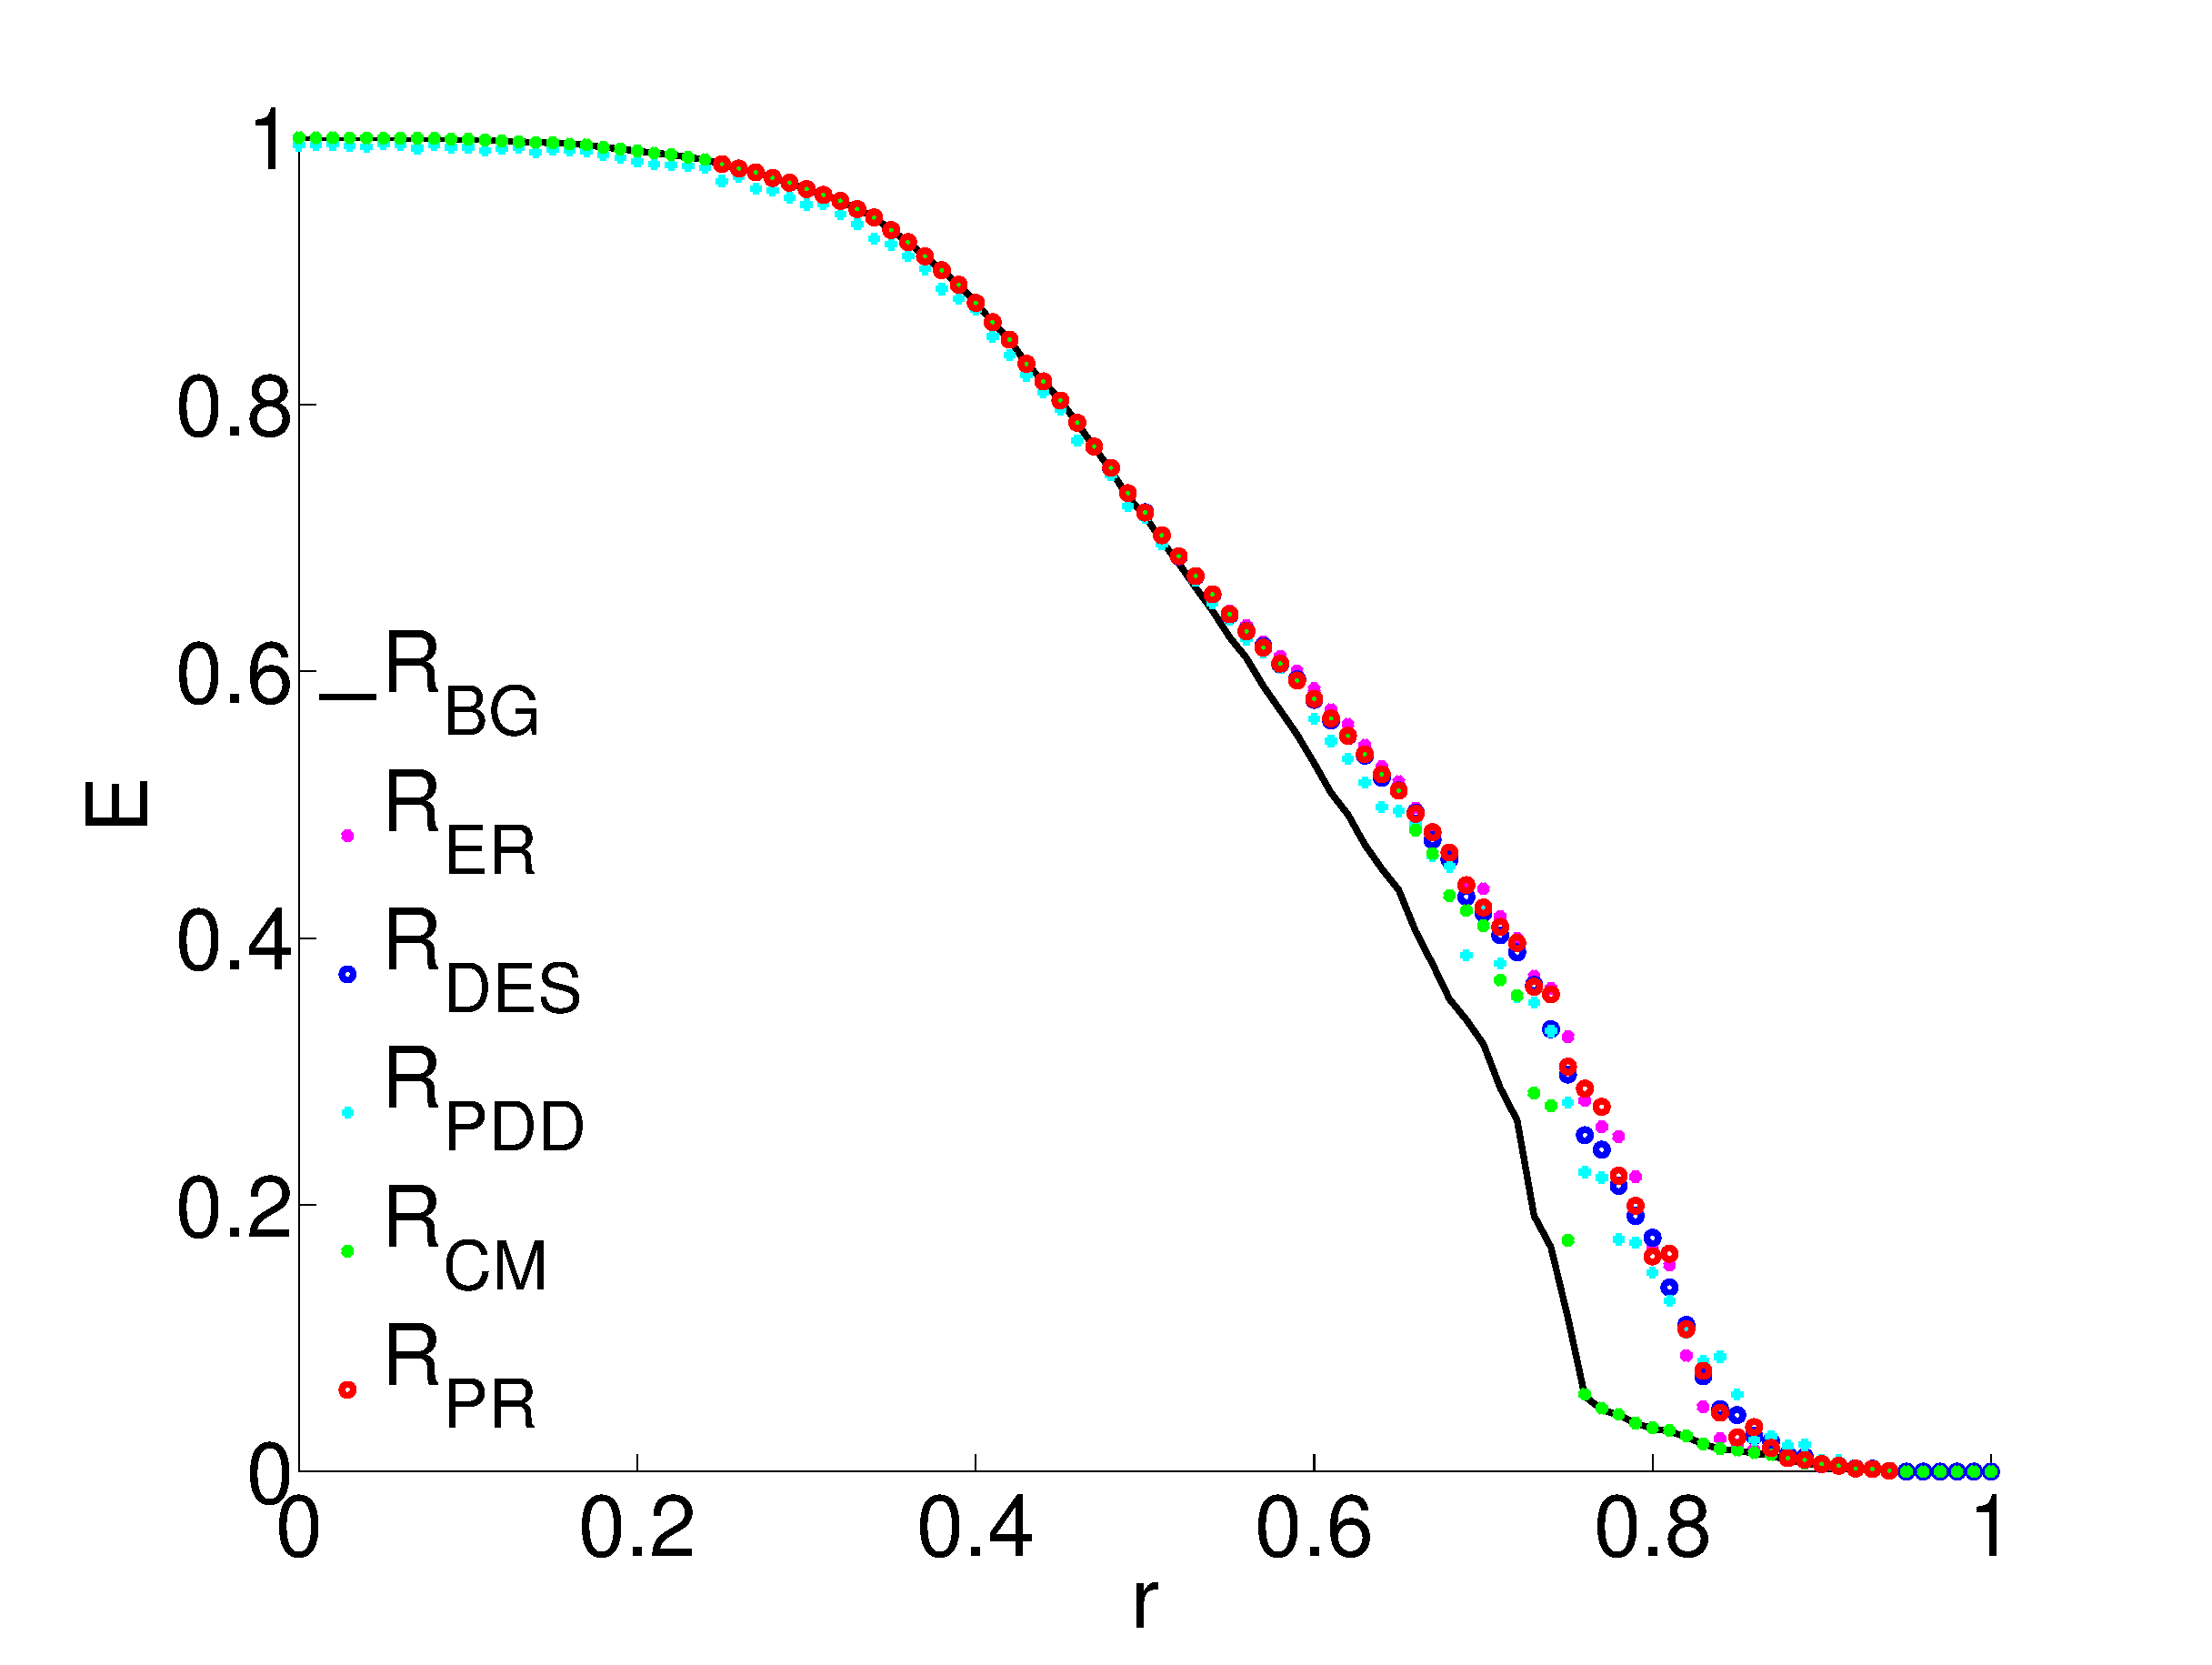
\includegraphics[width=0.45\textwidth, height=60mm]{Global_Efficiency_Average_Fnc.eps} &

    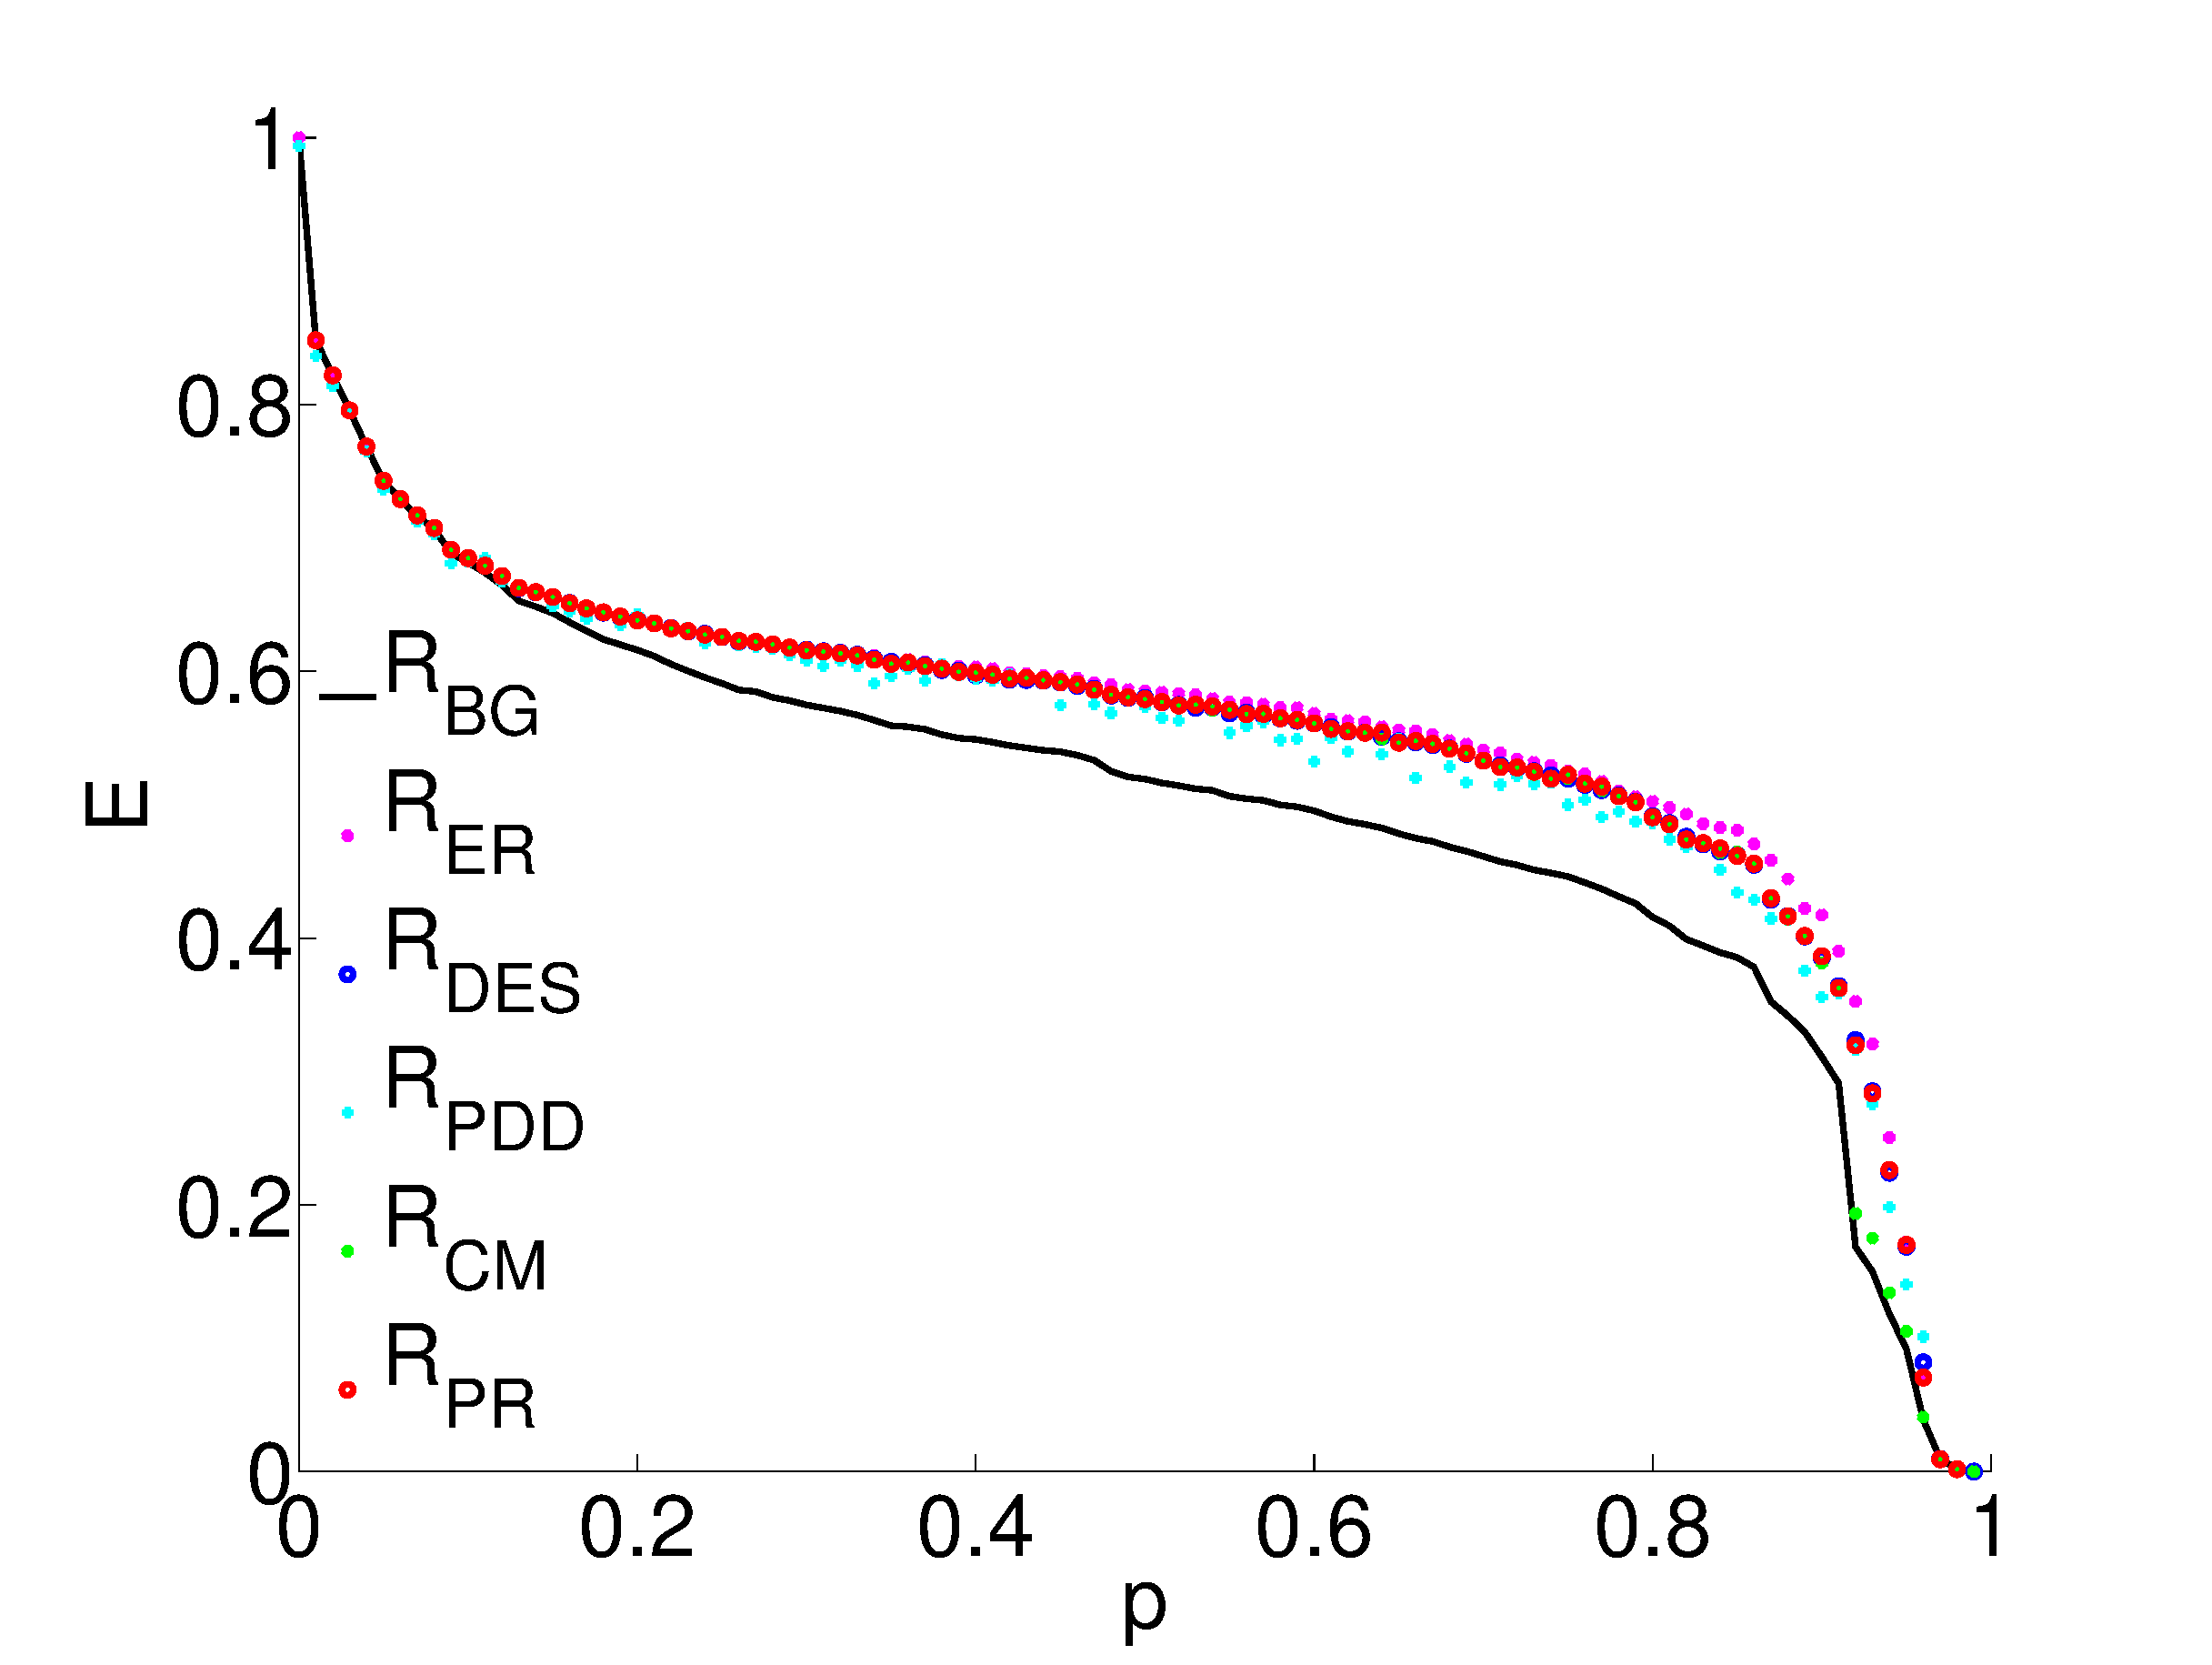
\includegraphics[width=0.45\textwidth, height=60mm]{Global_Efficiency_Average_Stru.eps}\\

  \end{tabular}

 \label{figur}\caption{Global efficiencies of the original networks and random graphs; FCM on left side, ACM on right side. }
 
\end{figure}

In figure 7, the random graph $Rk$ seems to have the lowest global efficiency and best matching global efficiency to the $R0$ for both FCM and ACM. Other random graphs have slightly larger global efficiency values than that of $R0$. 

When Figure 6 and Figure 7 are compared, one can see that higher  $d_{ij}$ values reveals lower global efficiency in a network. If it is easier to visit a node starting from any other node in the graph, the information transmission is better.
%
\subsection{Local Efficiency}
The local efficiency is measured as the average of inverse shortest pathways between nodes in neighborhood of a specific node (Latora and Marchiori, 2001);

\begin{equation}
E_{loc} = \frac{1}{n}\sum\limits_{i \epsilon N} E_{loc,i} = \frac{1}{n}\sum\limits_{i \epsilon N} \frac{\sum\limits_{j,h \epsilon N, j\neq i} a_{ij} a_{ih}[d_{jh}(N_i)]^{-1}}{k_i(k_i - 1) }
\end{equation}

where $E_{loc,i}$ is the local efficiency of node $i$, $d_{jh}(N_i)$ is the shortest pathway between nodes $j$ and $h$, which are located in neighborhood of node $i$. Local efficiency measure the ability of a network to transmit information at the local level (Latora and Marchiori, 2001, 2003).


\begin{figure}[htp]

  \centering

    \begin{tabular}{cc}

    % Requires \usepackage{graphicx}

    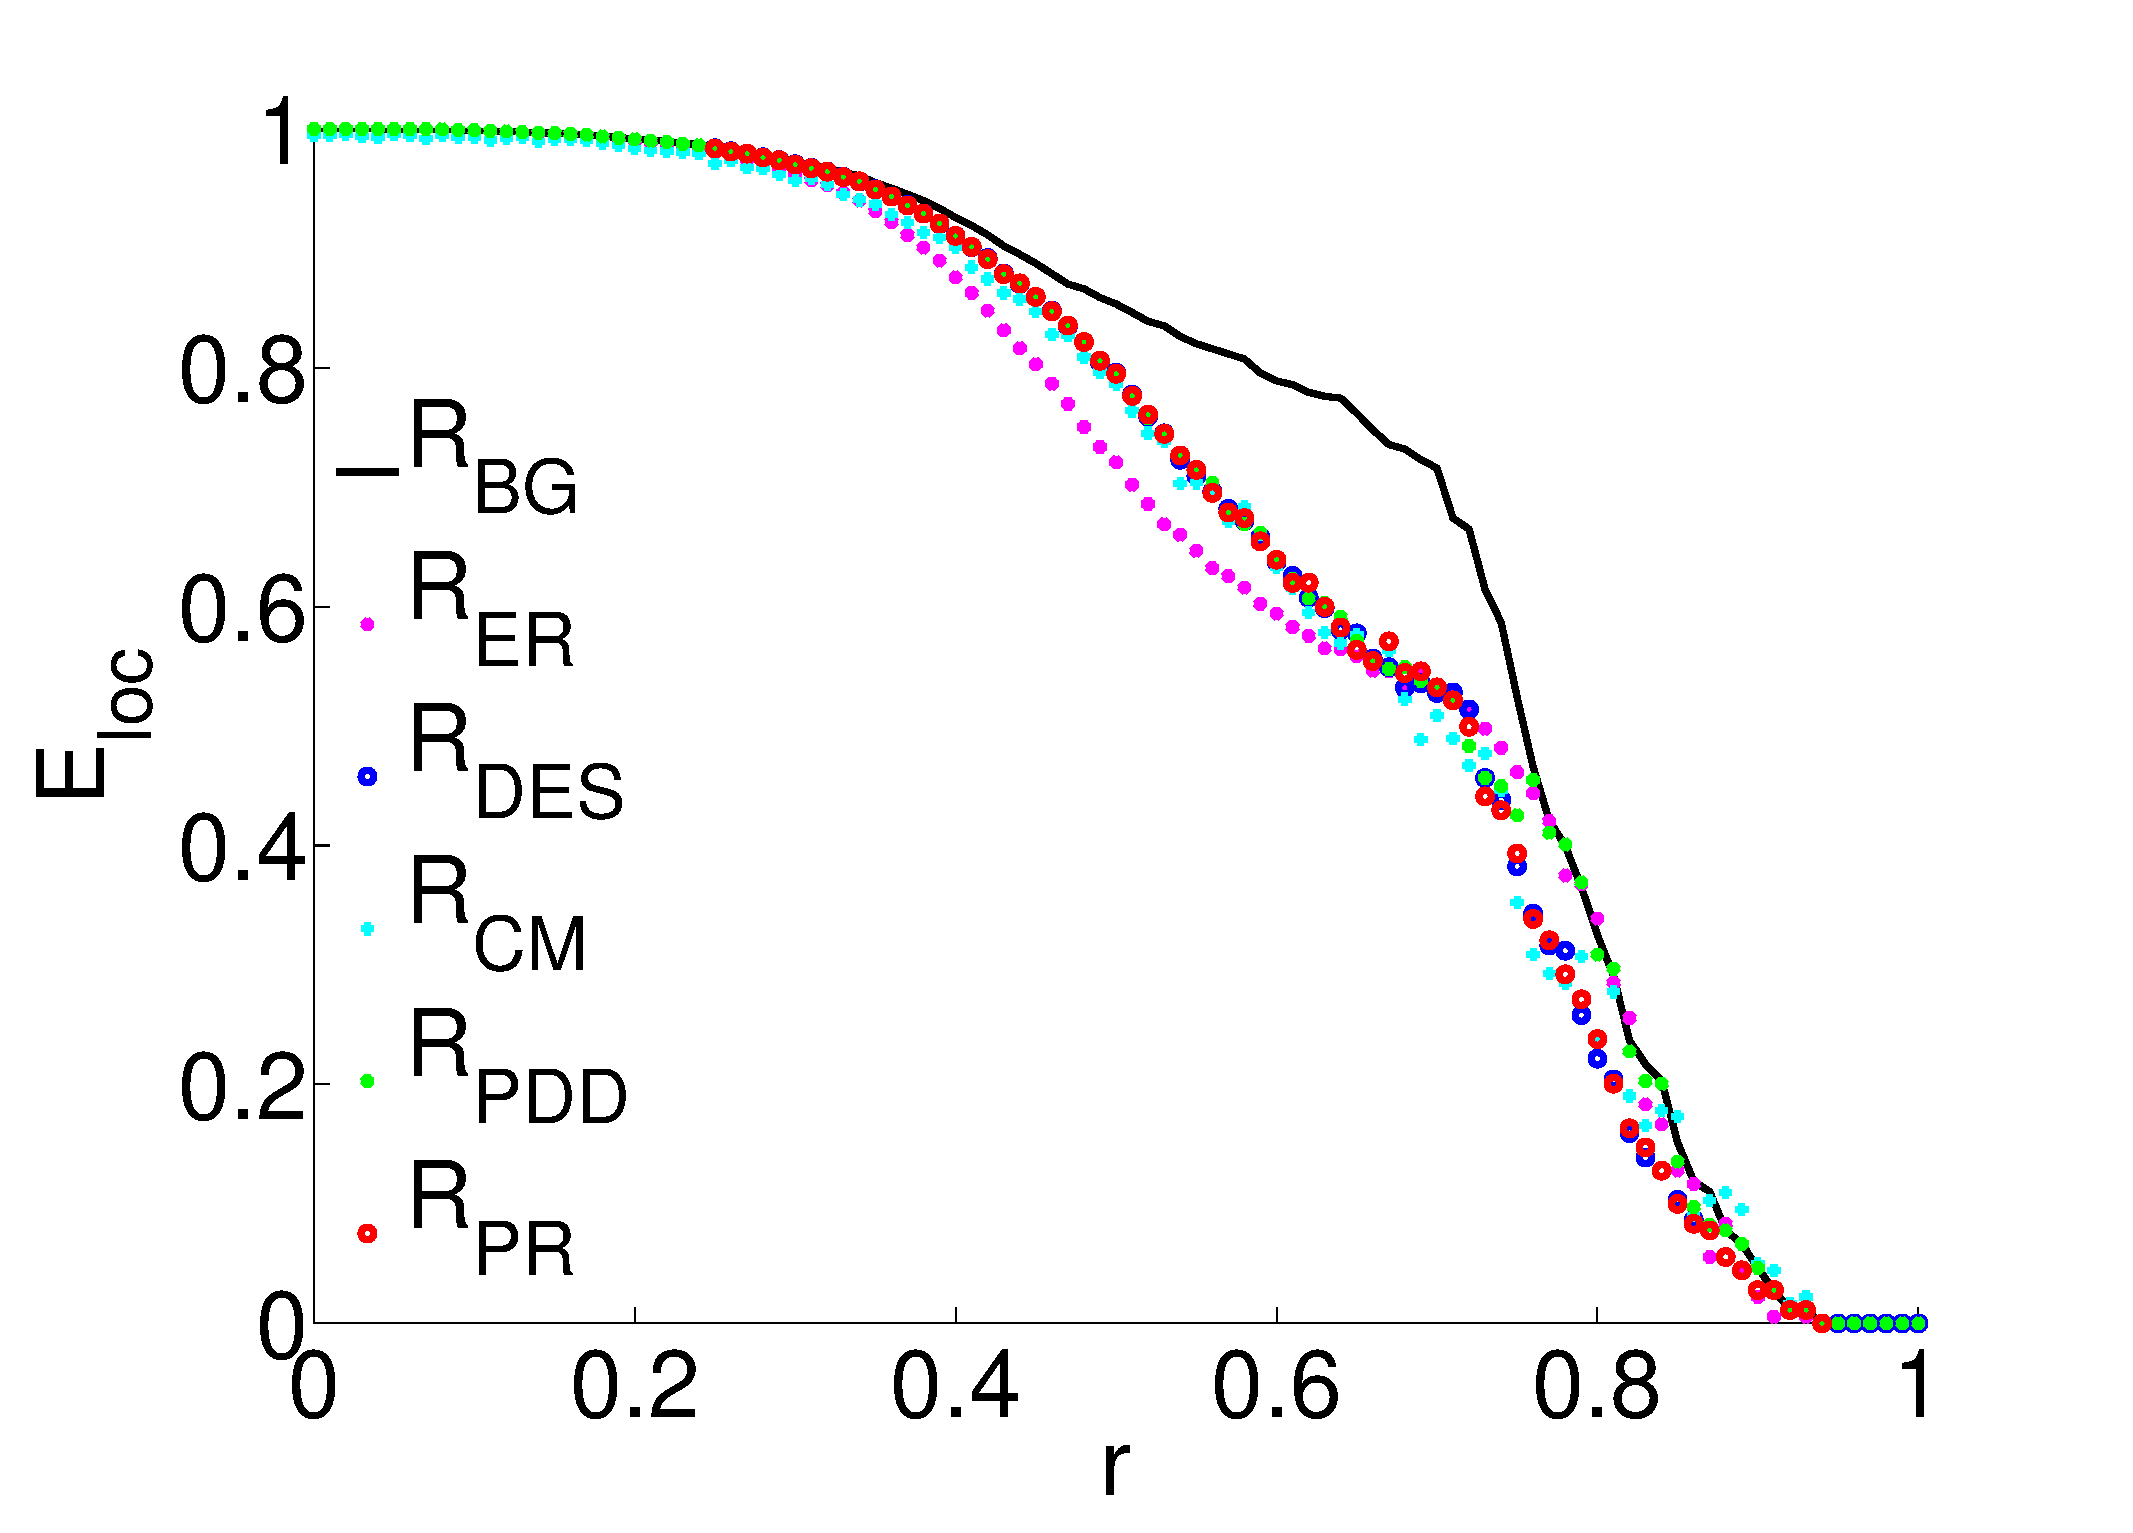
\includegraphics[width=0.45\textwidth, height=60mm]{Local_Efficiency_Average_Fnc.eps} &

    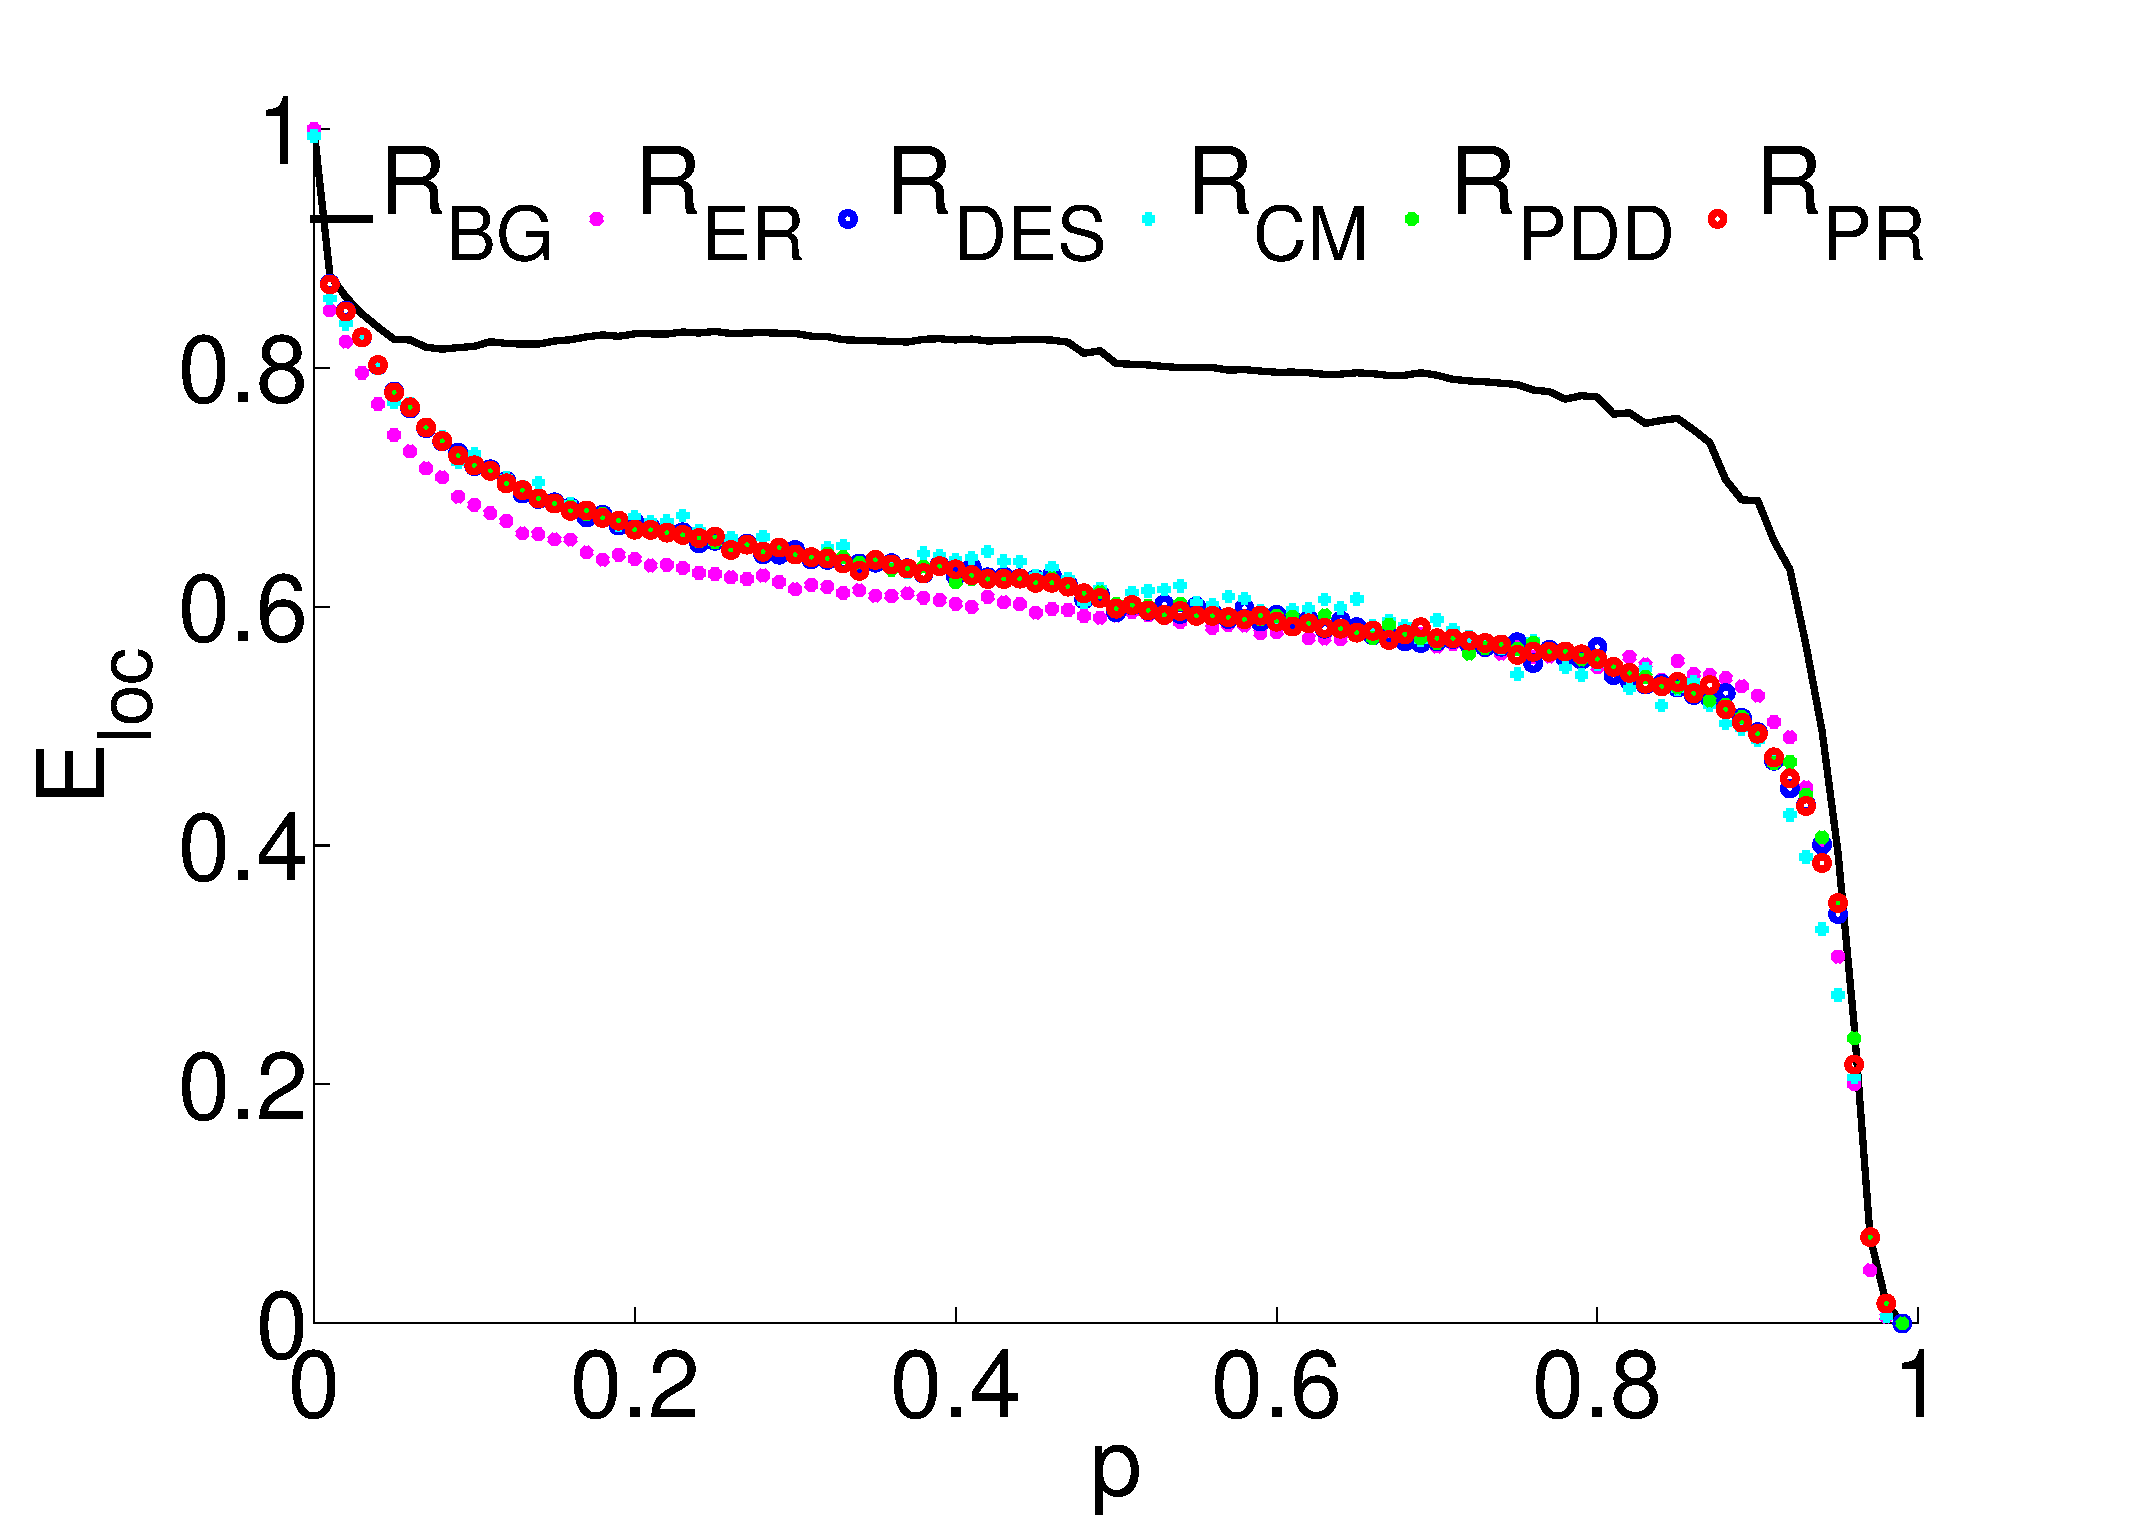
\includegraphics[width=0.45\textwidth, height=60mm]{Local_Efficiency_Average_Stru.eps}\\

  \end{tabular}

 \label{figur}\caption{Local efficiencies of the test networks and random graphs}
 
\end{figure}

The random graph $Rk$ and the actual graph $R0$ have relatively higher local efficiency than that of other random graphs for both FCM and ACM. The anatomical connectivity network and its random graphs have in general higher local efficiency compared to the functional connectivity network. In general local information transmit is more efficient in ACM than in FCM. The graphs having higher global efficiencies in Figure 7 tends to have lower local efficiencies in Figure 8. 

\newpage

\subsection{Small Worldness}

A small world network is both highly segregated and integrated, a measure of small worldness was proposed to capture this effect in a single statistic (Humpries and Gurney,2008).

\begin{equation}
S = \frac{C/C_{rand}}{L/L_{rand}}
\end{equation}
 
 where $C$ and $C_{rand}$ are clustering coefficients, $L$ and $L_{rand}$ are characteristic path lengths of the original and random network respectively. The random network here is constructed with \textit{Erdos-Renyi} method, which has the same number of nodes and links as the reference graph. 

\begin{equation}
L = \frac{1}{n}\sum\limits_{i \epsilon N} L_i = \frac{1}{n}\sum\limits_{i \epsilon N} \frac{\sum\limits_{j \epsilon N, j \neq i }d_{ij}}{n-1 } 
\end{equation}

\begin{figure}[htp]

  \centering

    \begin{tabular}{cc}

    % Requires \usepackage{graphicx}

    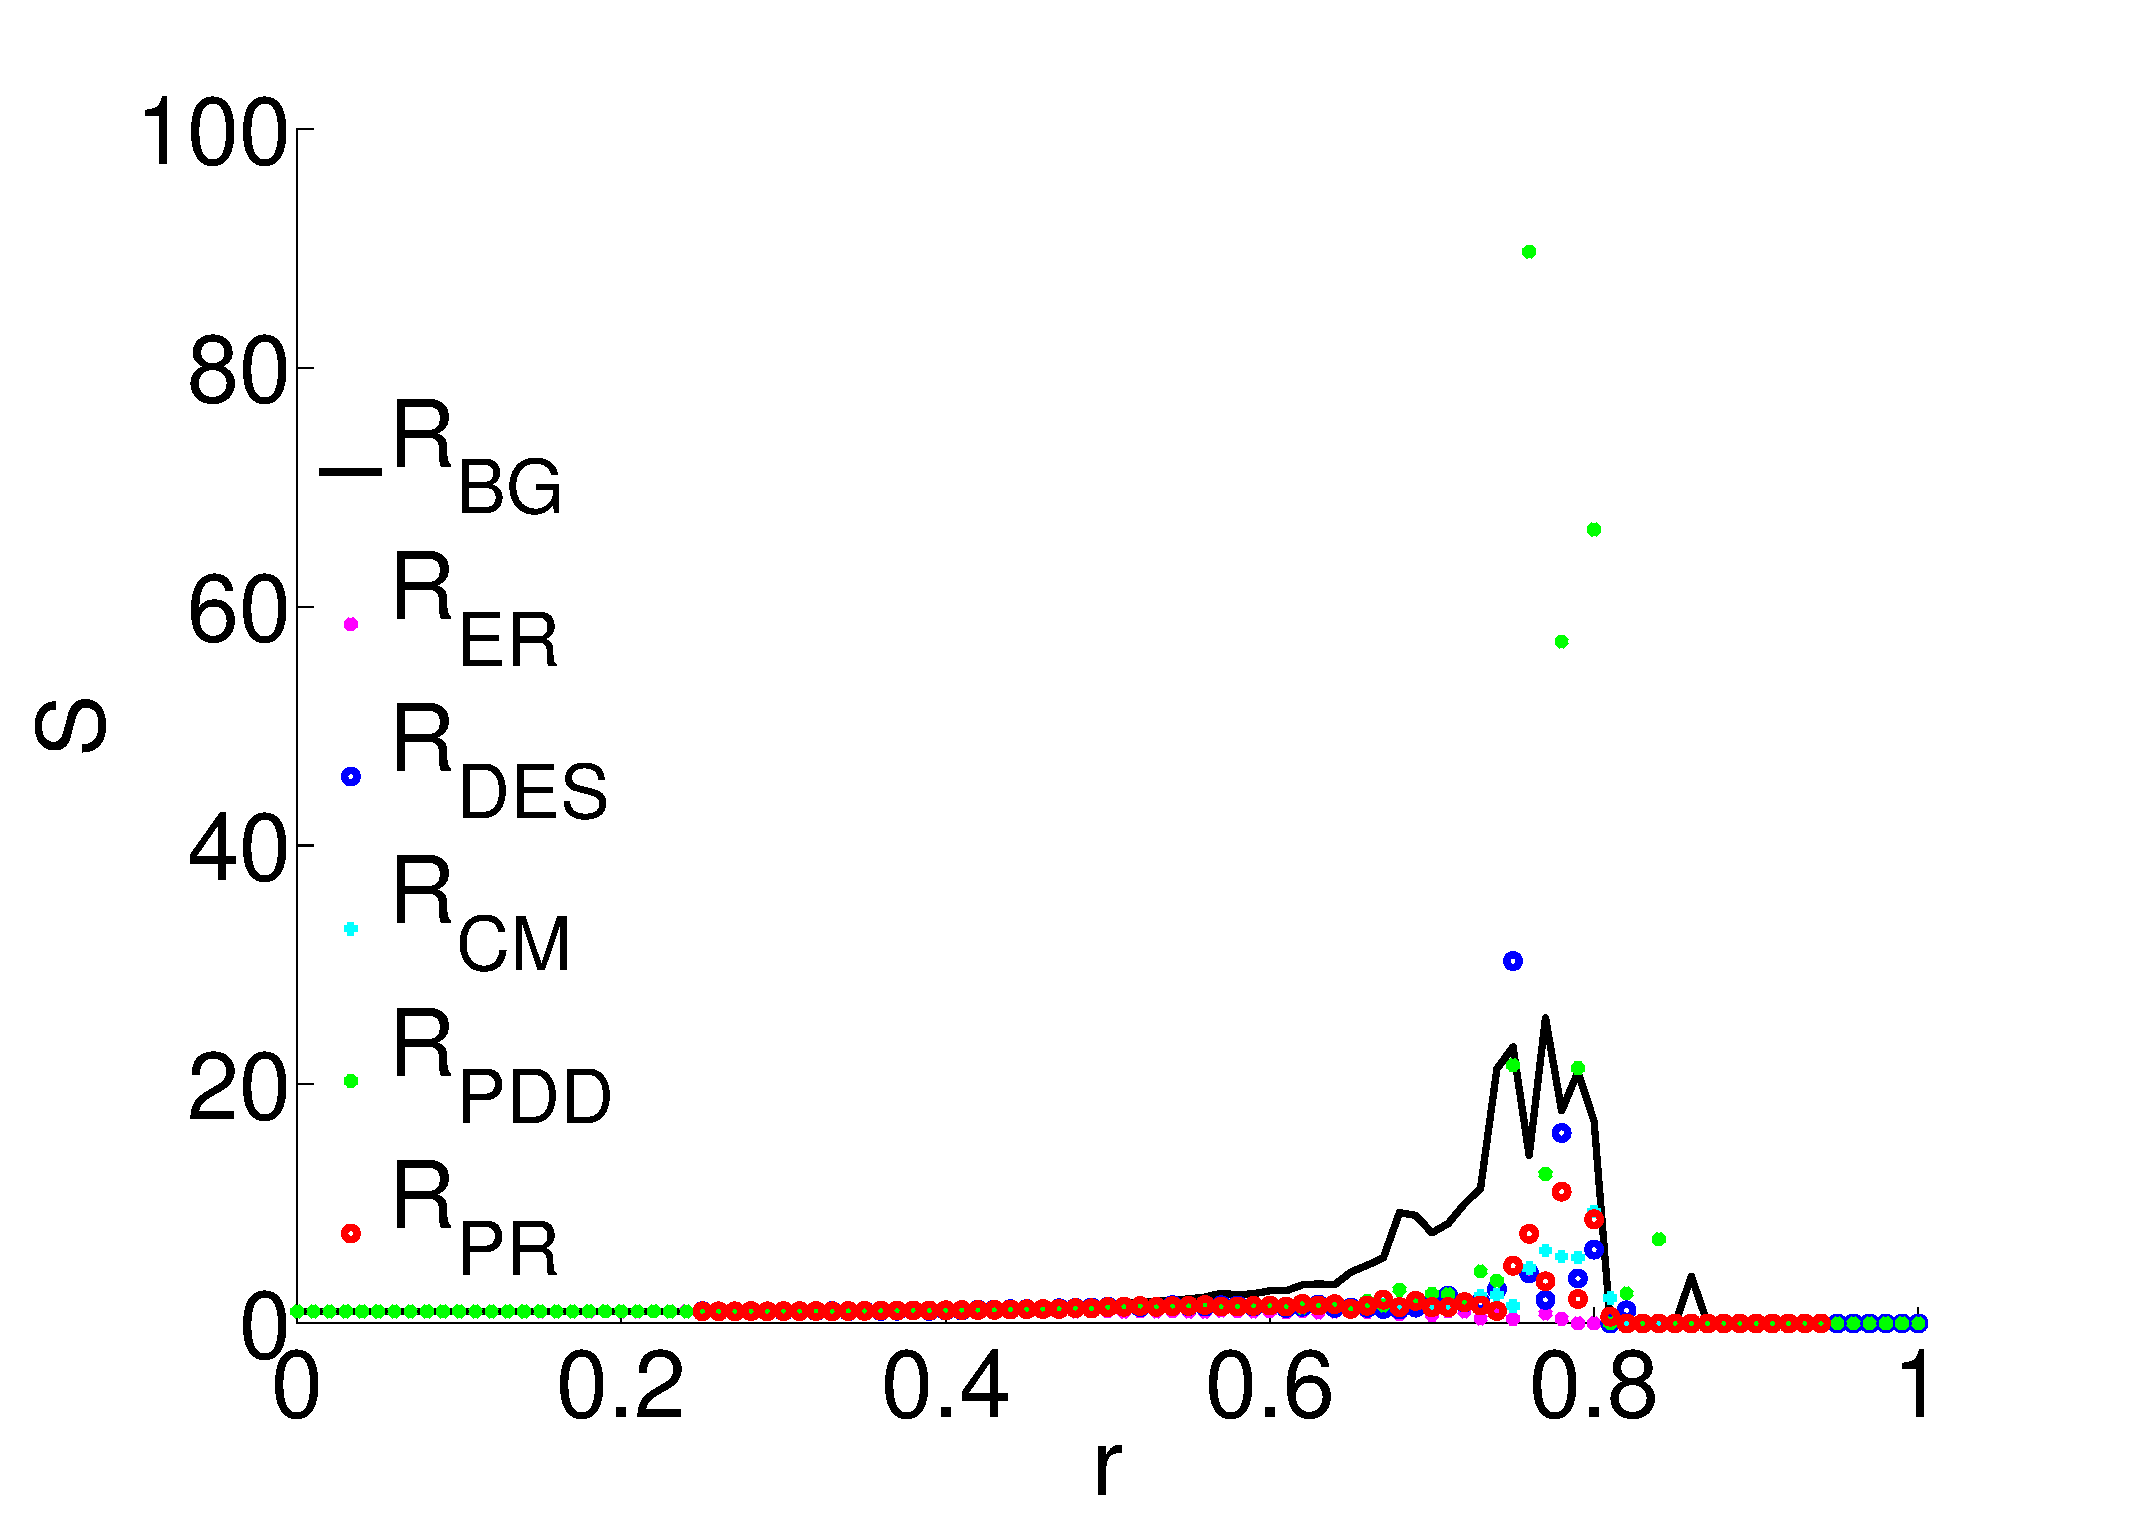
\includegraphics[width=0.45\textwidth, height=60mm]{Small_Worldness_Fnc.eps} &

    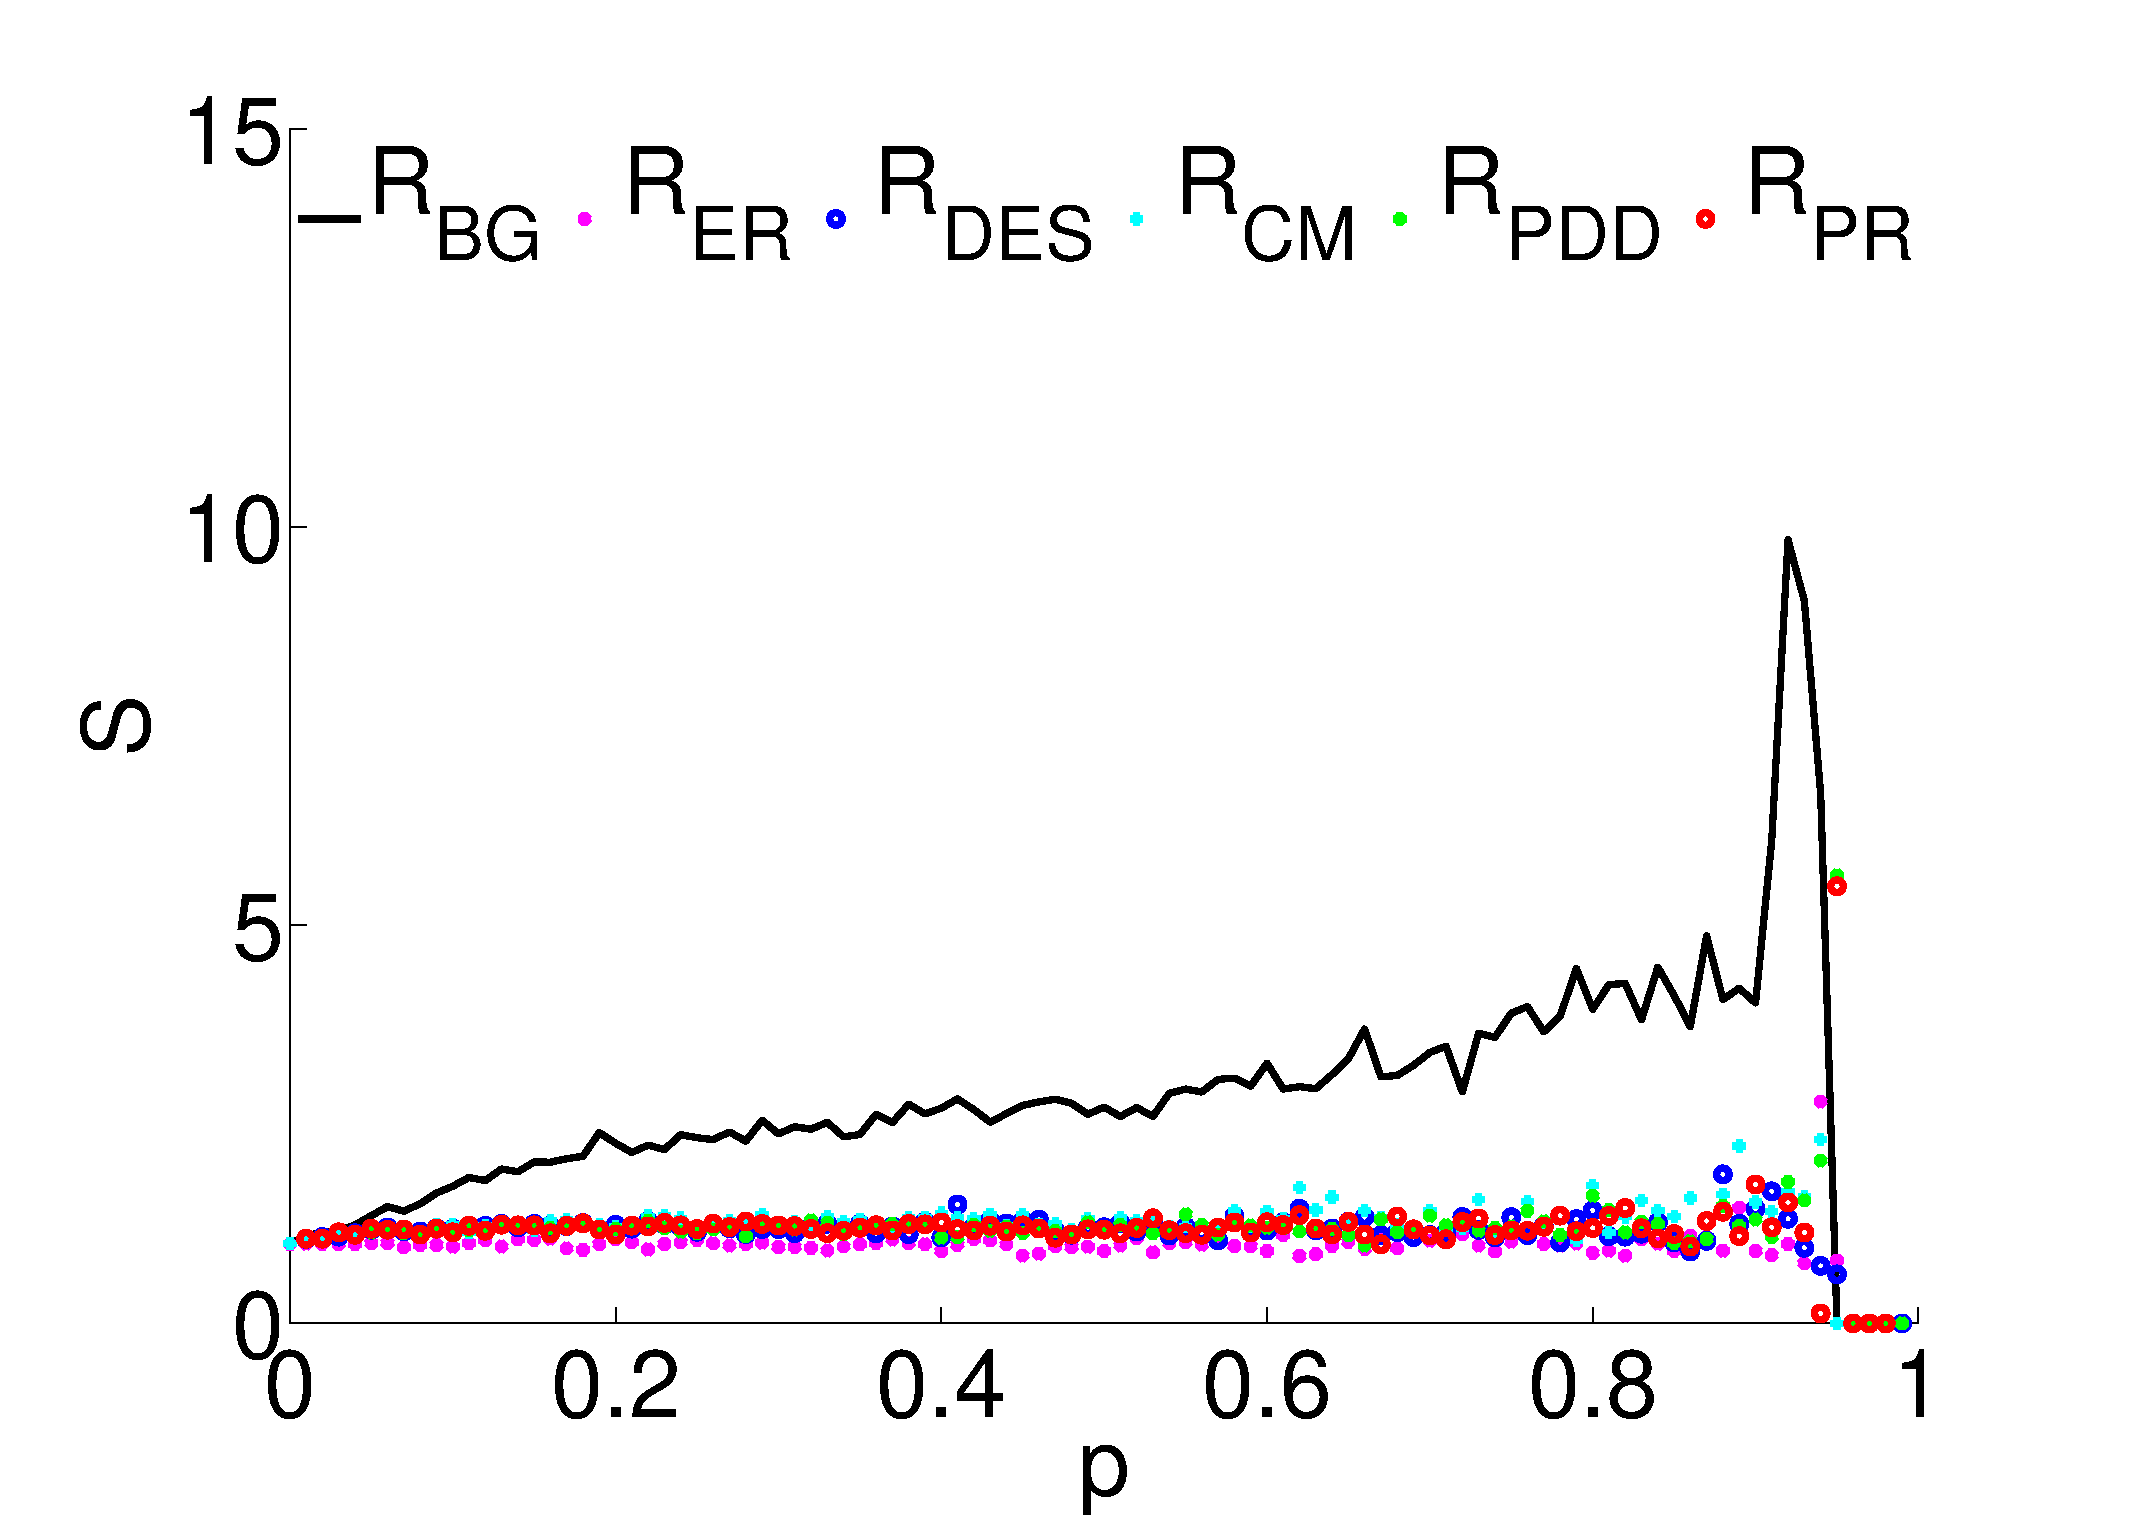
\includegraphics[width=0.45\textwidth, height=60mm]{Small_Worldness_Stru.eps}\\

  \end{tabular}

 \label{figur}\caption{Small worldness of the test networks and random graphs.  }
 
\end{figure}


In Figure 9, $Rk$ graph has the highest small worldness among other random graphs for both FCM and ACM. The usual best matching pattern between $R0$ and $Rk$ is lost, when small worldness is measured.

Figure 3 representing cluster coefficients show that the $R0$ and $Rk$ networks have larger $C$ than the other randomly constructed networks. The characteristic pathway $L$ is truly proportional with the shortest pathway $d_{ij}$. Figure 6 gives a hint that $R0$ network tend to have smaller $d_{ij}$, indicating smaller characteristic pathway for it.The division in equation 8 results in such an $S$ value, much larger 1.

Figure 10 implies that the random networks except for $Rk$ can not be equally segregated and integrated at the same time. The real world networks $R0$ for both  FCM and ACM tend to have higher small worldness, however $Rk$ reaches the highest values only at some $p$ and $r$ values.  

\subsection{Assortativity}

Assortativity measures the correlation coefficient between the degrees of all nodes on two opposite ends of a link [RUB10]. Assortativity coefficient of the network (Newman, 2002);

\begin{equation}
A = \frac{\dfrac{1}{l} \sum\limits_{(i,j) \in L}  k_i k_j -  \Big ( \dfrac{1}{2L} \sum\limits_{(i,j) \in L}k_i + k_j  \Big )^2}{\dfrac{1}{2L}\sum\limits_{(i,j) \in L} ( k_i^2+  k_j^2) -\Big ( \dfrac{1}{2L} \sum\limits_{(i,j) \in L}k_i + k_j  \Big )^2 }
\end{equation}

where $L$ is number of edges in, $k_i$ is degree of node $i$.


\begin{figure}[htp]

  \centering

    \begin{tabular}{cc}

    % Requires \usepackage{graphicx}

    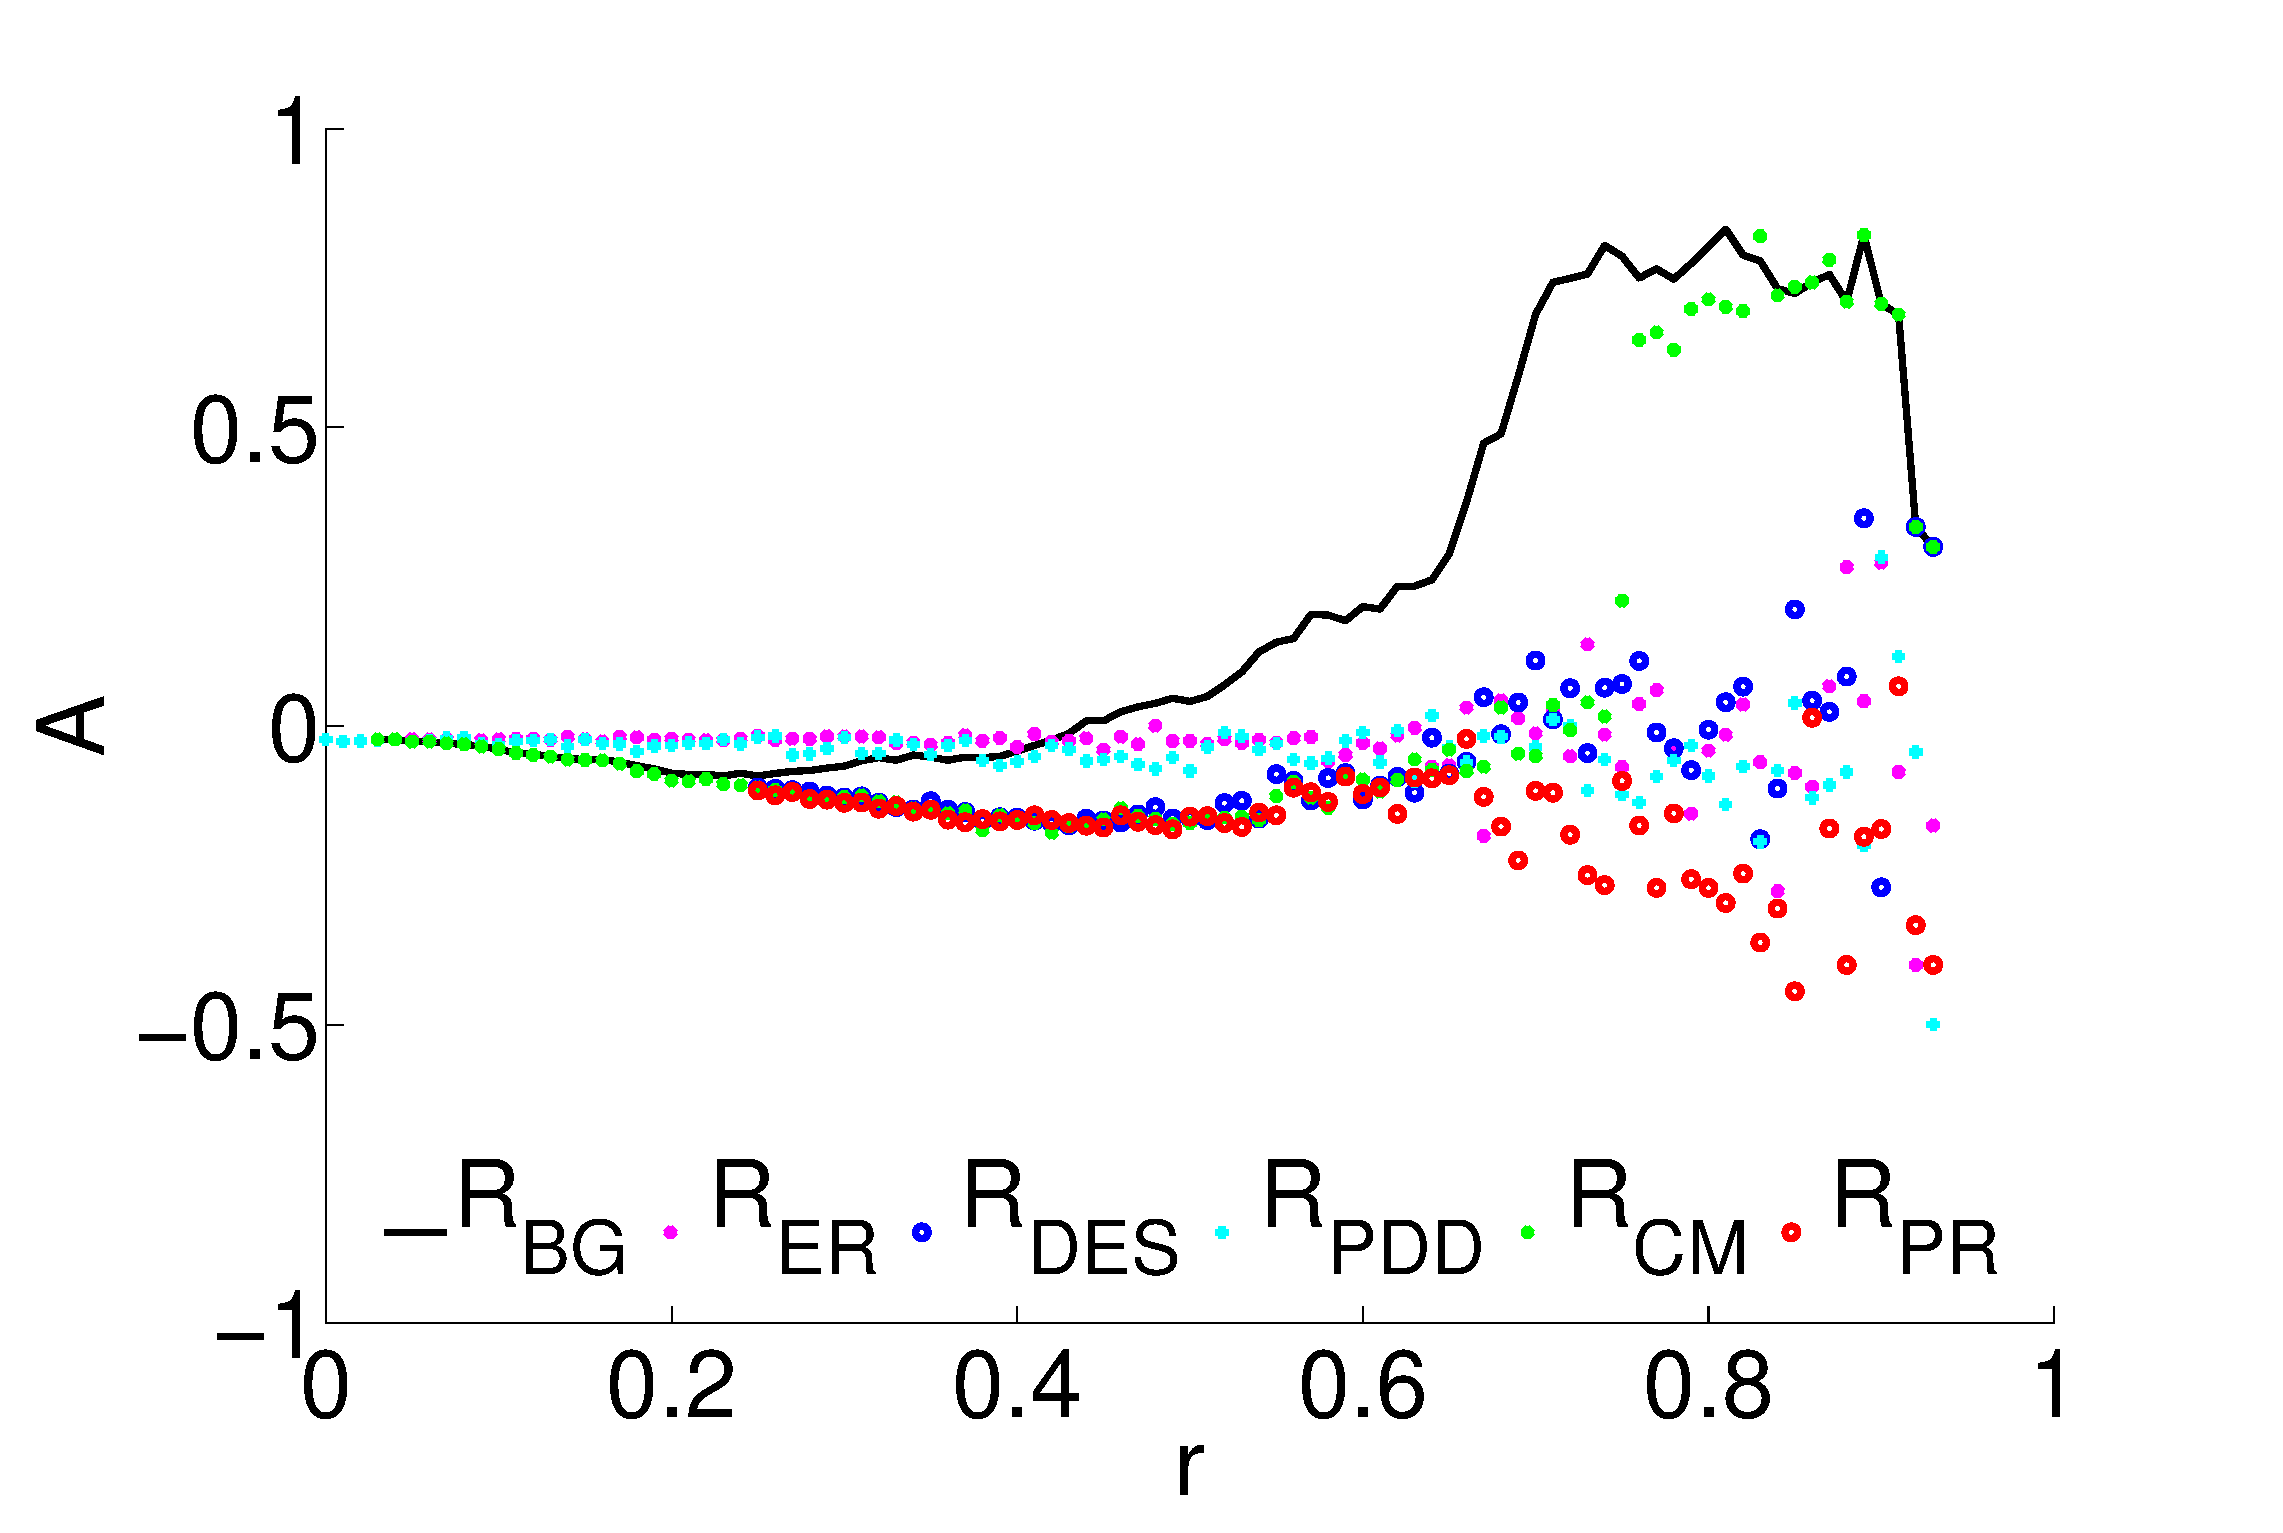
\includegraphics[width=0.45\textwidth, height=60mm]{Assortativity_Fnc.eps} &

    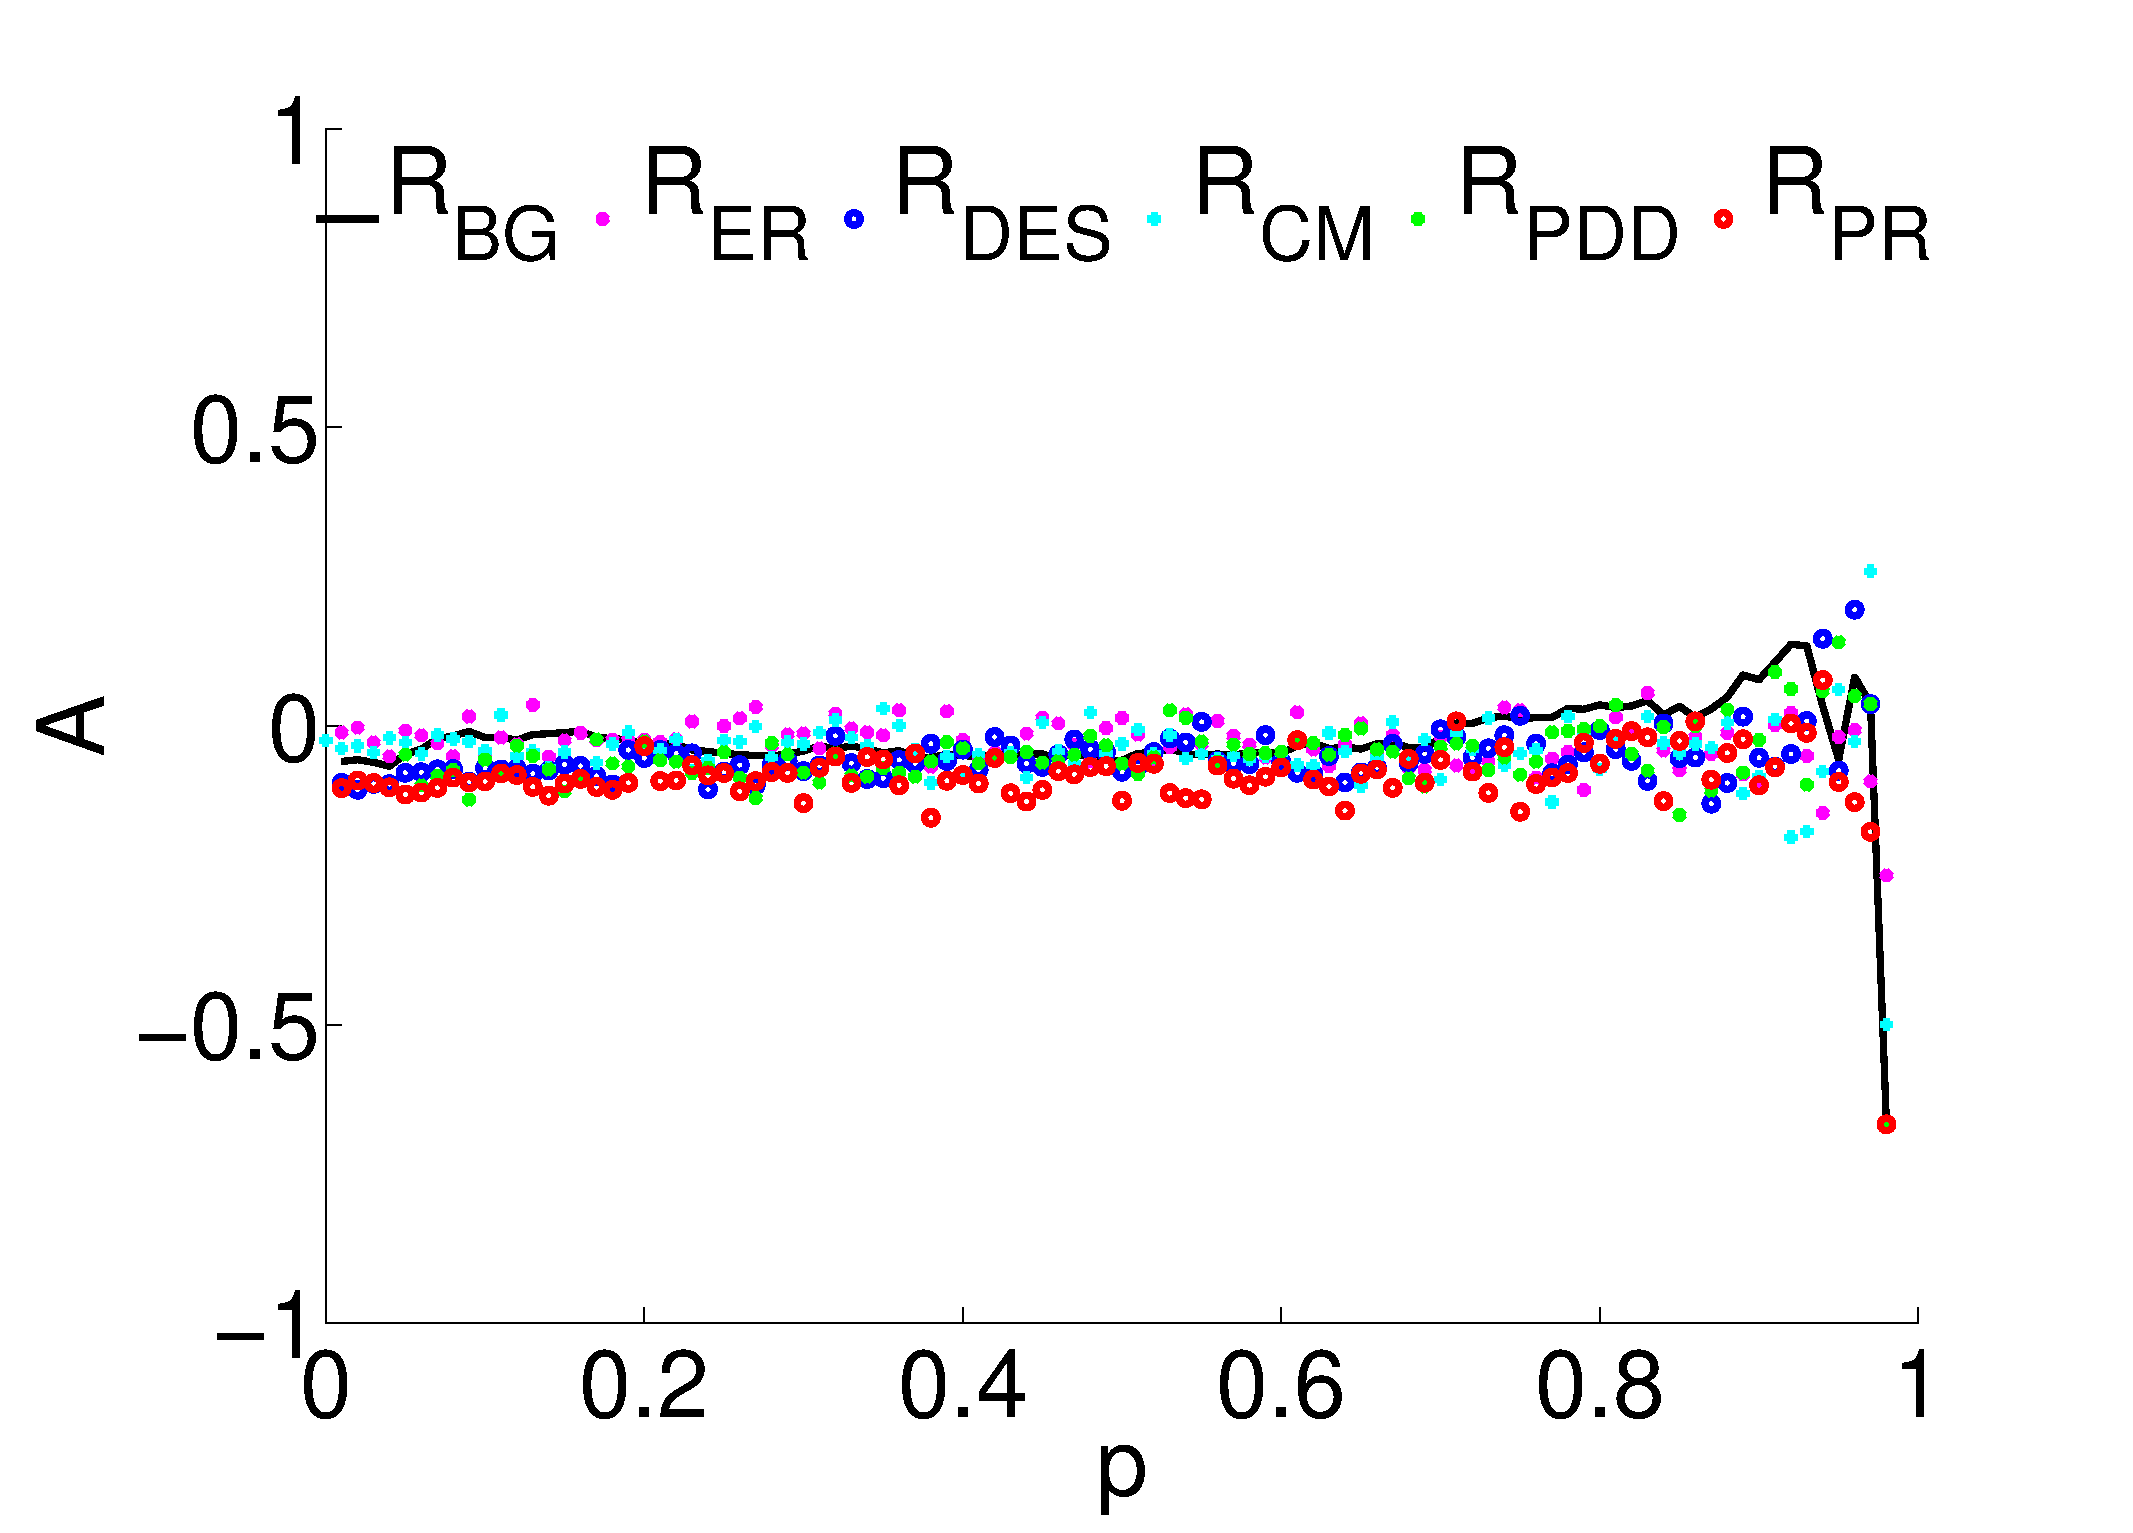
\includegraphics[width=0.45\textwidth, height=60mm]{Assortativity_Stru.eps}\\

  \end{tabular}

 \label{figur}\caption{Assortativity coefficients of the $R0$ networks and random graphs}
 
\end{figure}

In Figure 10, $R0$ and $Rk$ graphs have the highest assortativity in general for FCM. However, assortativity values tend to be very similar for all the graphs in ACM. 

Negative assortativity presents a network having widely distributed high-degree hubs [RUB10]. On the other hand, assortativity coefficients close to $1$ indicates a graph having fine correlated degree nodes. 

\newpage

\subsection{Degree Distribution}
Degree distribution of a network reflects the probability ($P$) of a node to have a given number of degree ($k$). Degree distribution reveals the resilience of a graph. 

\begin{equation}
 P(k) = \sum\limits_{k' \geq k} p(k')
\end{equation}

where $p(k')$ is the probability of a node having degree $k'$ (Barabasi and Albert, 1999). 

\begin{figure}[htp!]
	\centering
	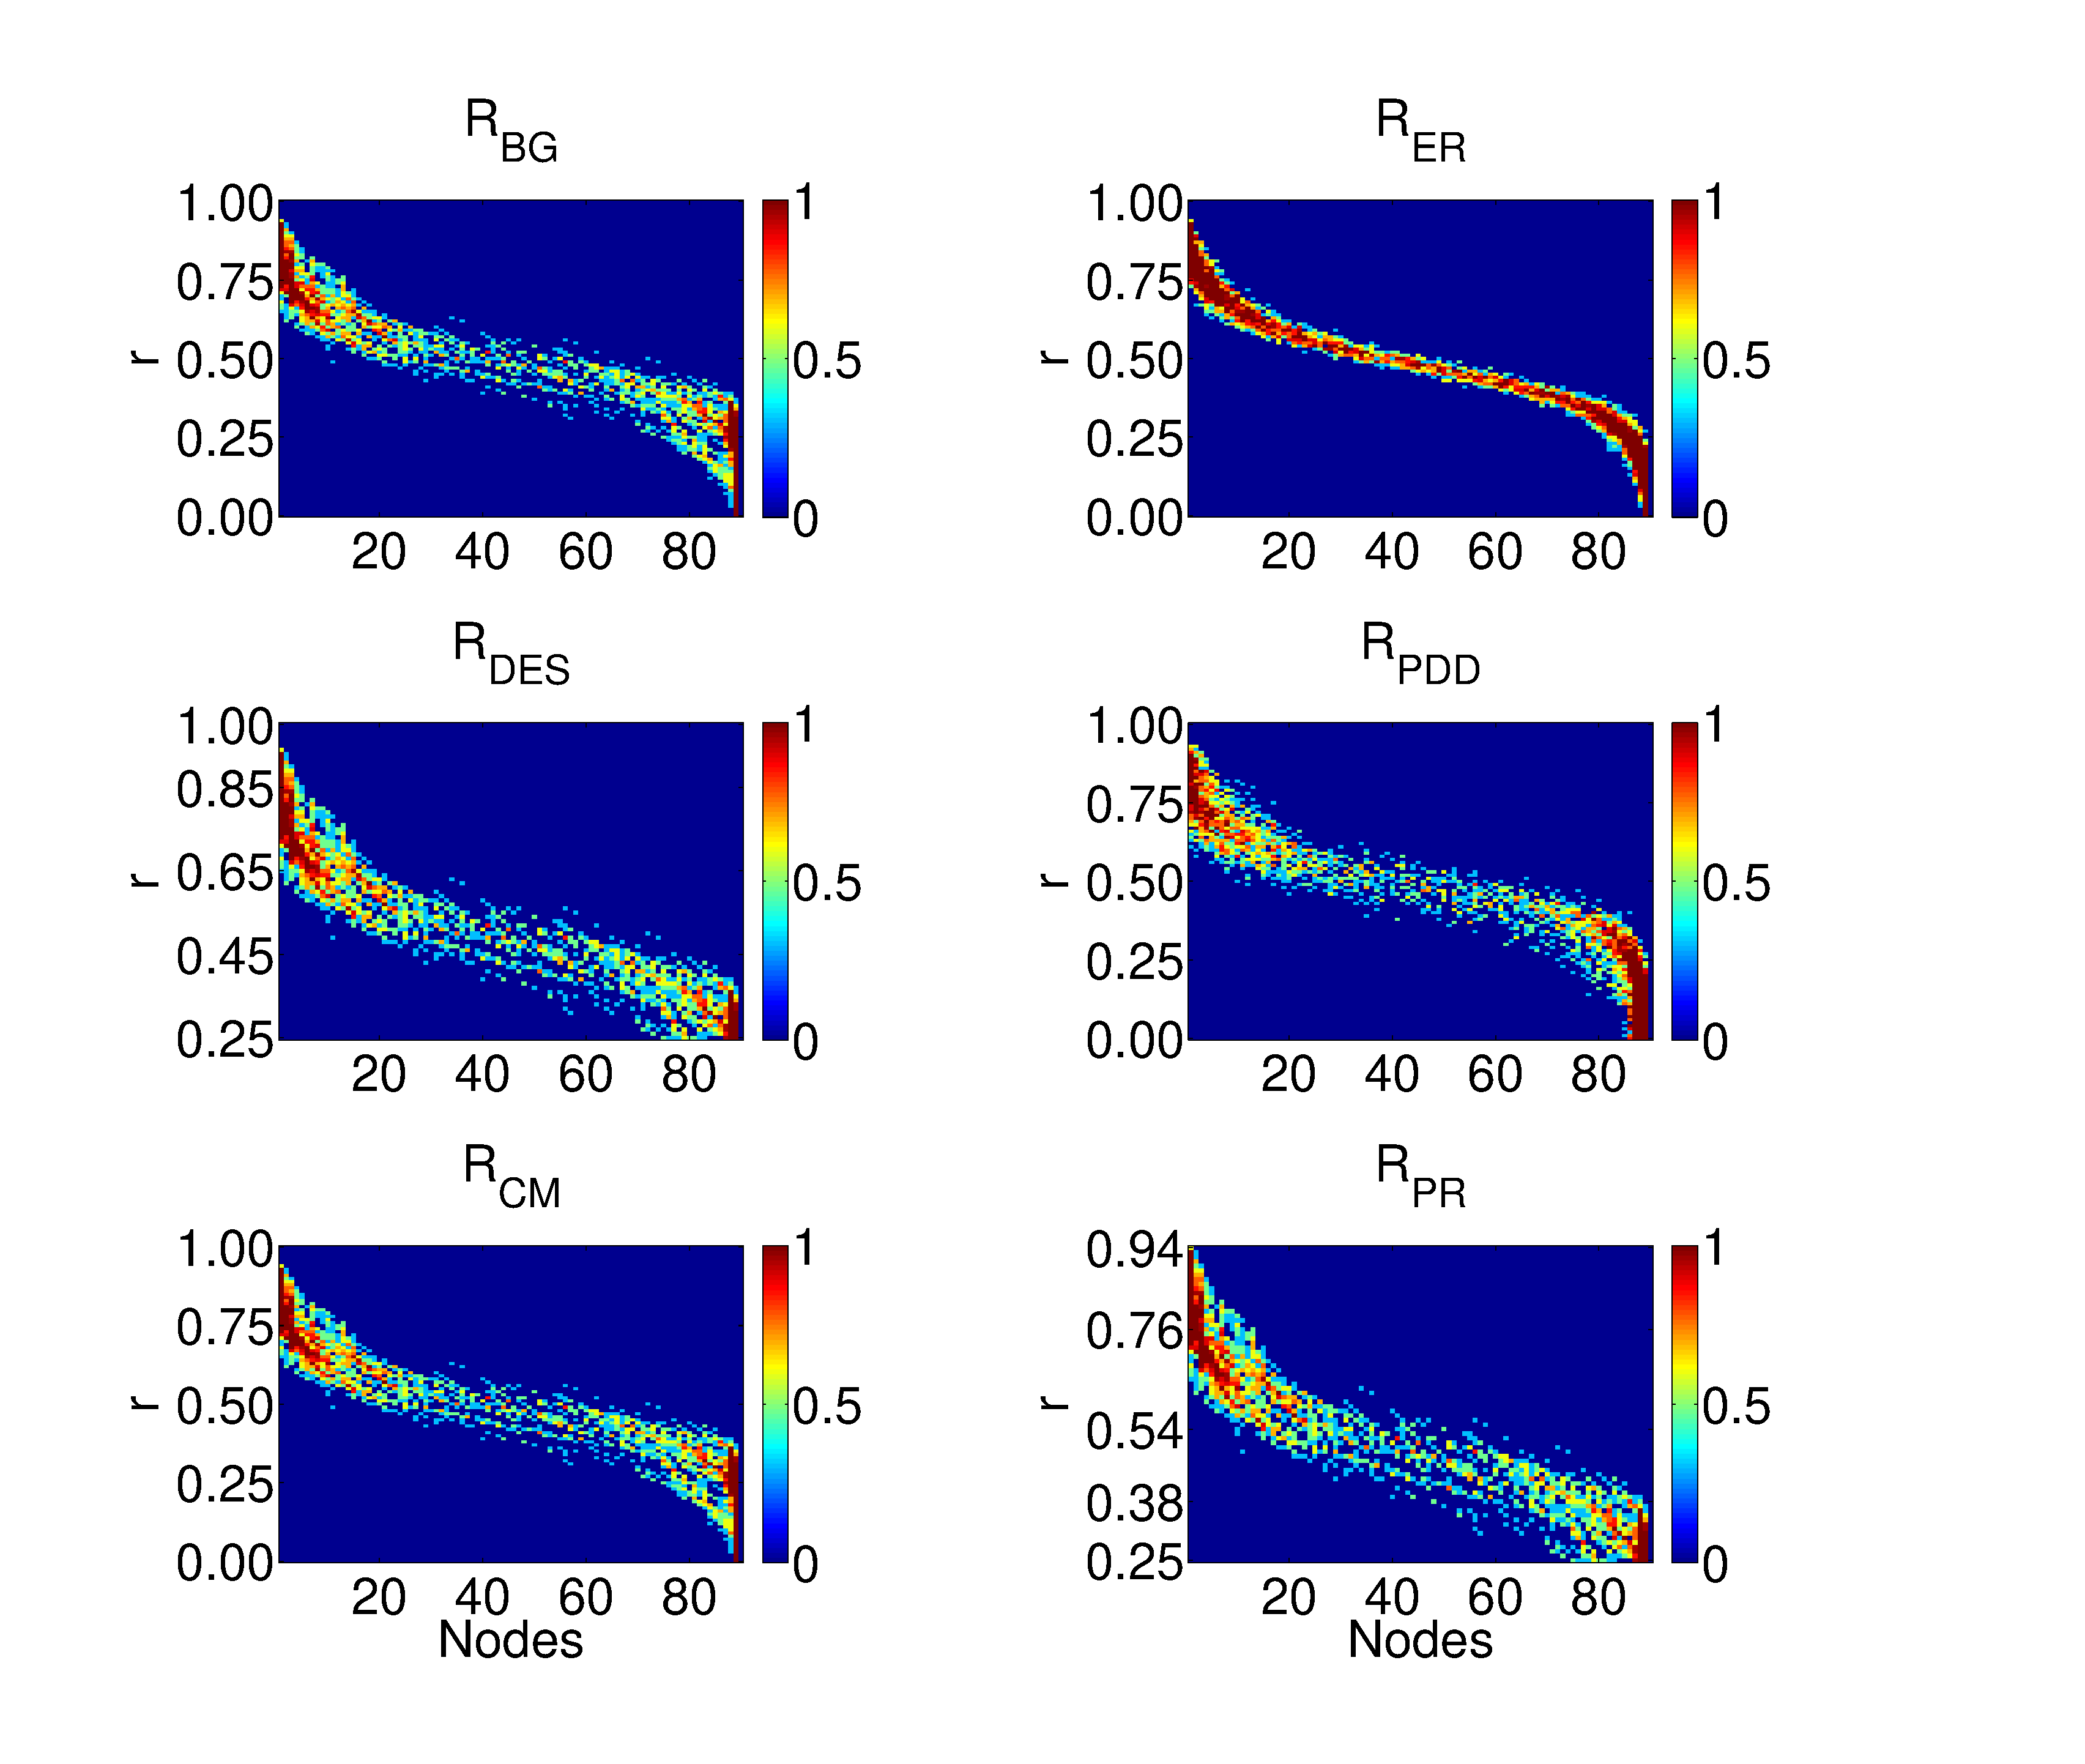
\includegraphics[width=140mm]{Degree_Distribution_Fnc.eps}
	\caption{Heat maps of degree distributions of the FCM network. The limits of colorbar are $[log_{10}(10^0), log_{10}(10^1)]$.}
\end{figure}

\newpage

\begin{figure}[h!]
	\centering
	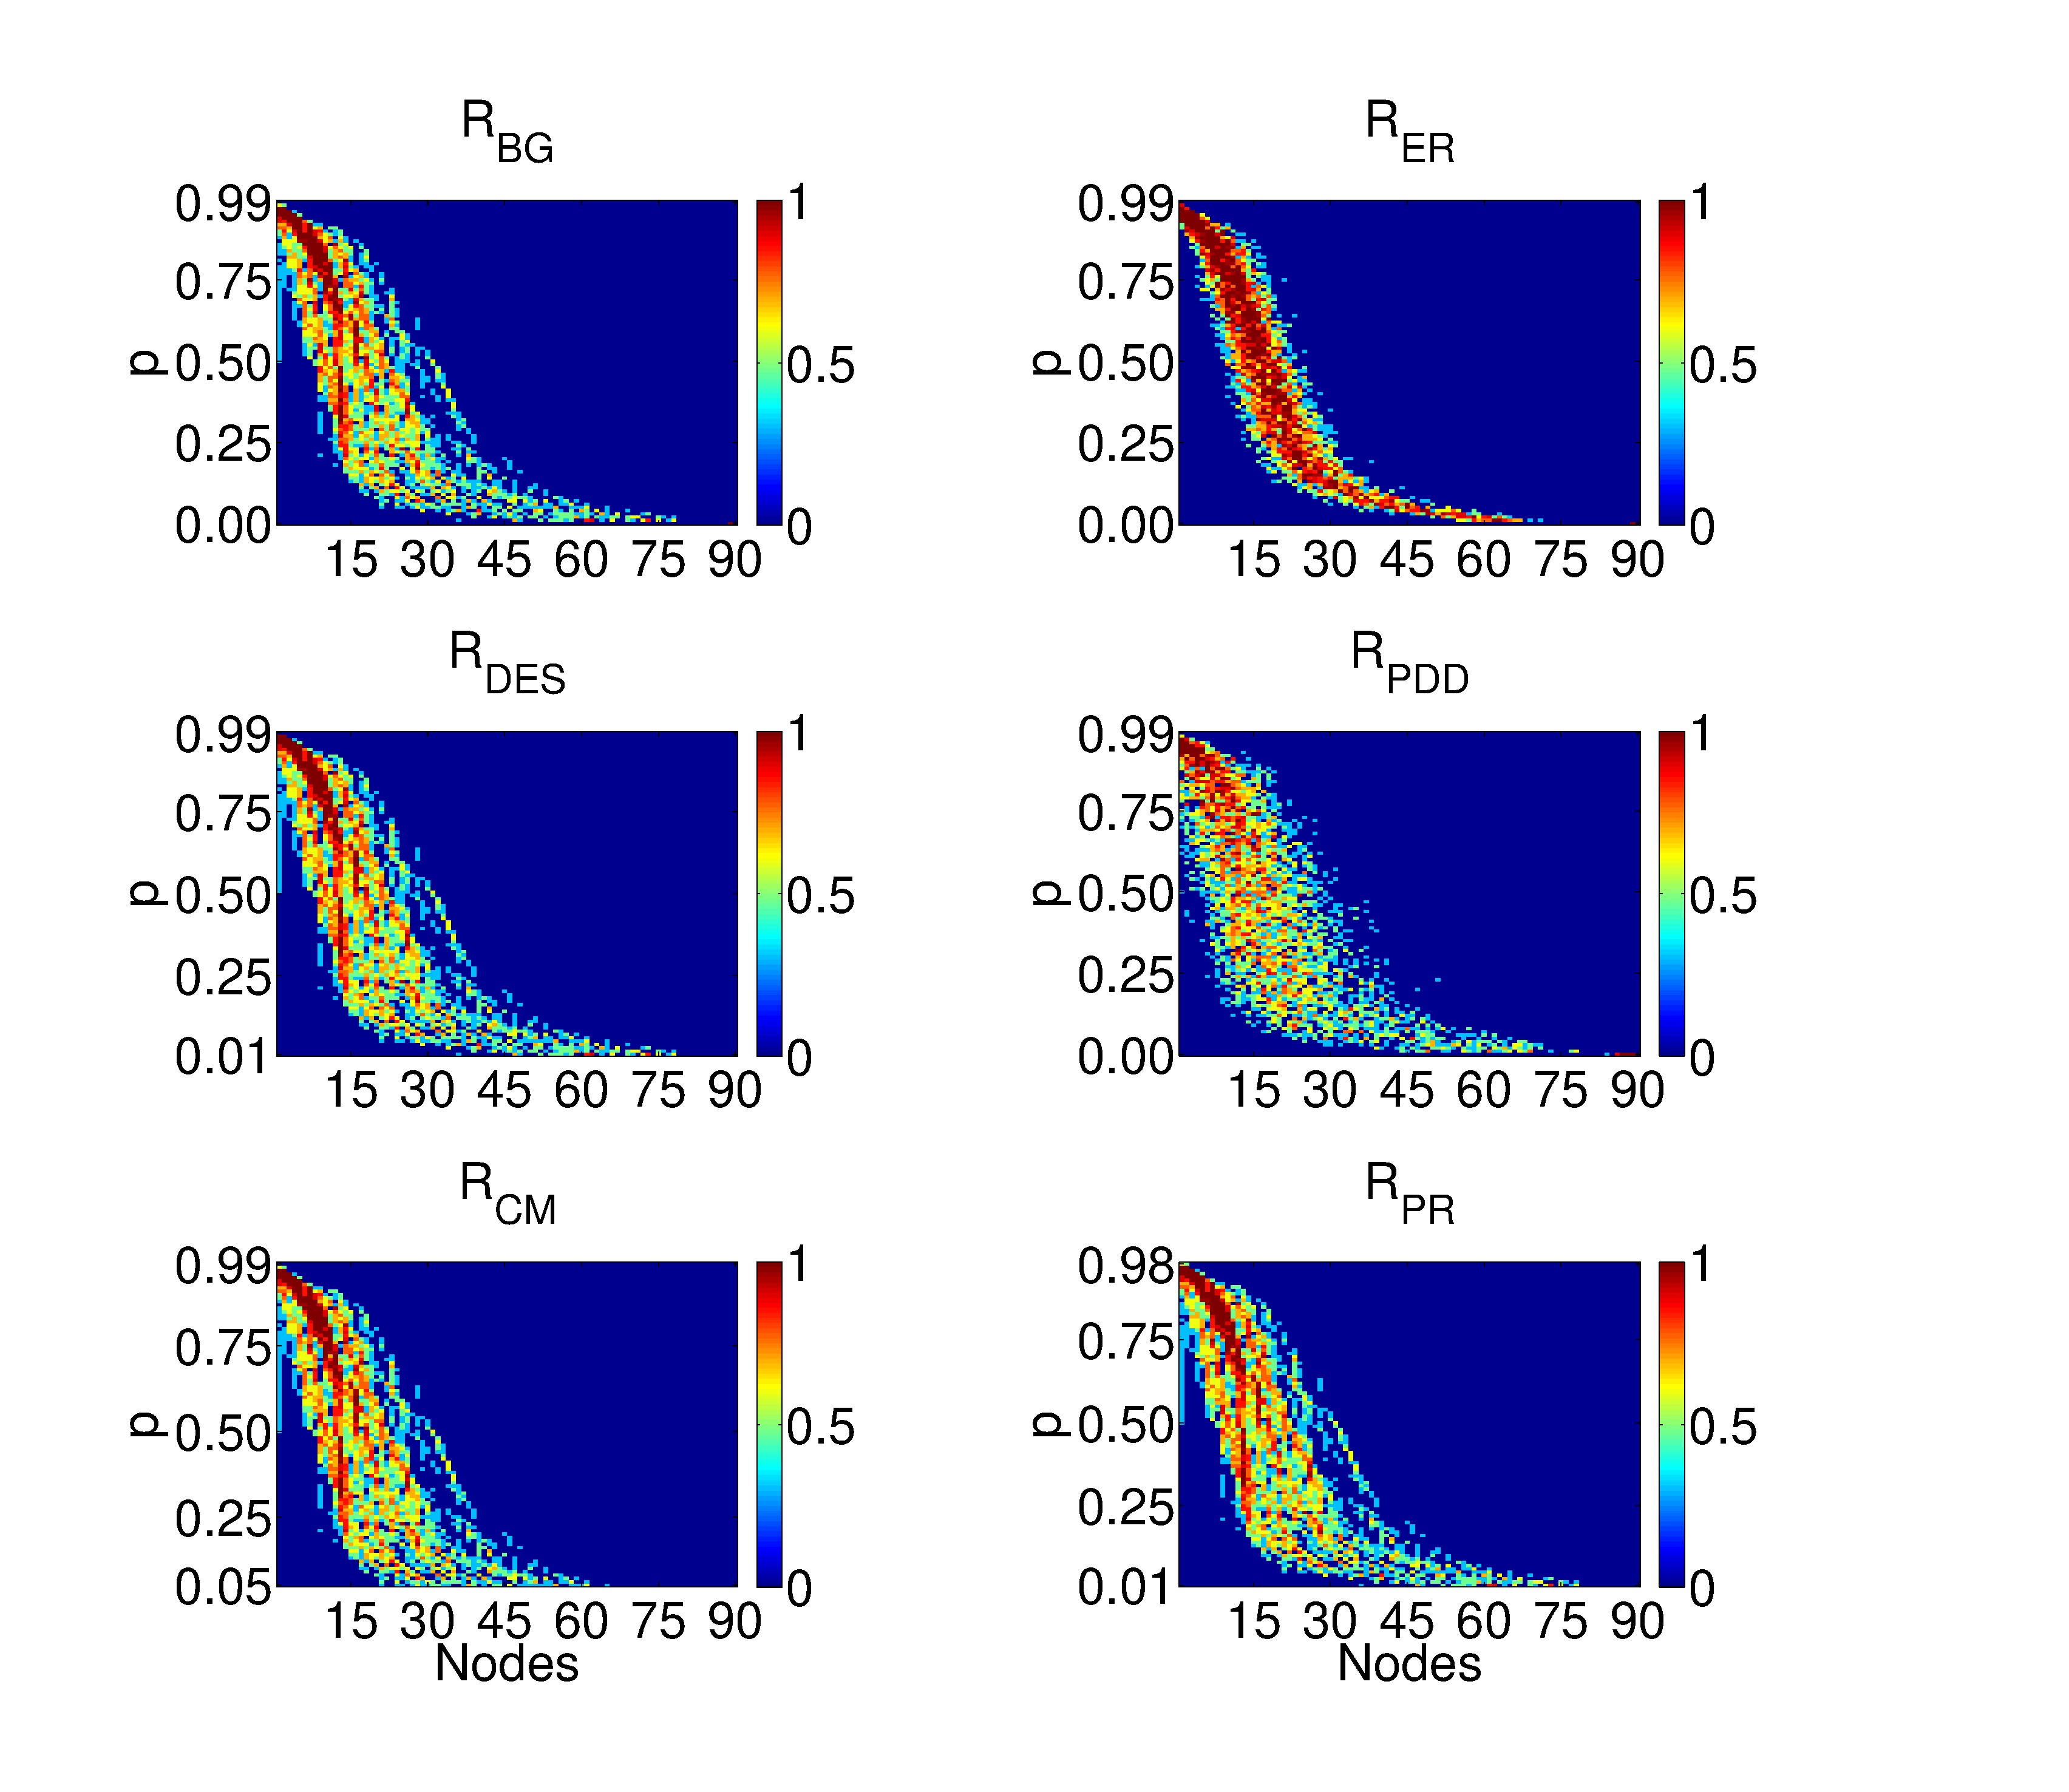
\includegraphics[width=\textwidth]{Degree_Distribution_Stru.eps}
	\caption{Heat maps of degree distributions of the ACM network and the randomized networks. The colors are coded as logarithmic scale. The limits of colorbar are $[log_{10}(10^0), log_{10}(10^1)]$. }
\end{figure}

\newpage

\subsection{Clustering Coefficient of Nodes}

The clustering coefficient of each node is measured as ratio between number of triangles around a node and all possible edge connections of that node ${k_i \choose 2} $ (Watts and Stogatz, 1998); 

\begin{equation}
C_i =  \frac{2t_i}{k_i(k_i -1)}
\end{equation}

As the number of triangles around a node increased, $C_i$ becomes larger indicating more segregated nodes in the network.


\begin{figure}[h!]
	\centering
	\includegraphics[width=140mm]{Clustering_Coefficient_Node_Fnc.eps}
	\caption{Heat maps of clustering coefficient distributions of FCM network.}
\end{figure}

\newpage

\begin{figure}[h!]
	\centering
	\includegraphics[width=\textwidth]{Clustering_Coefficient_Node_Stru.eps}
	\caption{Heat maps of clustering coefficient distributions of ACM network.}
\end{figure}

\newpage

\subsection{Connected Components of Nodes}
Connected components of nodes tells us how many connections a single node in any subgraph in its isolated neighborhood has. It implies how many other nodes we can reach through that single node. 



\begin{figure}[h!]
	\centering
	\includegraphics[width=\textwidth]{Connected_Components_Nodes_Fnc.eps}
	\caption{Heat maps of connected component distributions of FCM network. The colors are coded in logarithmic scale, the limits are $[log_{10}(10^0), log_{10}(10^2)]$.}
\end{figure}

\newpage

\begin{figure}[h!]
	\centering
	\includegraphics[width=\textwidth]{Connected_Components_Nodes_Stru.eps}
	\caption{Heat maps of connected component distributions of ACM network. The colors are coded in logarithmic scale, the limits are $[log_{10}(10^0), log_{10}(10^2)]$. The color codes are again in logarithmic scale but connected components are mostly 1, corresponding to blue color $10^0$.}
\end{figure} 

\newpage

\subsection{Global Efficiencies of Nodes}
Global efficiency of single node can be expressed with the following equation as described previously; 

\begin{equation}
 E_i =  \frac{\sum\limits_{j \epsilon N, j\neq i}d_{ij}^{-1}}{n-1 }
\end{equation}



\begin{figure}[h!]
	\centering
	\includegraphics[width=\textwidth]{Global_Efficiency_Nodes_Fnc.eps}
	\caption{Heat maps of global efficiency distributions of FCM network.}
\end{figure}

\newpage 


\begin{figure}[h!]
	\centering
	\includegraphics[width=\textwidth]{Global_Efficiency_Nodes_Stru.eps}
	\caption{Heat maps of global efficiency distributions of ACM network.}
\end{figure}

\newpage 

\subsection{Local Efficiency of Nodes}

\begin{equation}
 E_{loc,i} = \frac{\sum\limits_{j,h \epsilon N, j\neq i} a_{ij} a_{ih}[d_{jh}(N_i)]^{-1}}{k_i(k_i - 1) }
\end{equation}




\begin{figure}[h!]
	\centering
	\includegraphics[width=\textwidth]{Local_Efficiency_Nodes_Fnc.eps}
	\caption{Heat maps of local efficiency distributions of FCM network.}
\end{figure}

\begin{figure}[h!]
	\centering
	\includegraphics[width=\textwidth]{Local_Efficiency_Nodes_Stru.eps}
	\caption{Heat maps of local efficiency distributions of ACM network.}
\end{figure}

asdfasdfasdf\cite{RUB09}asdfasdfasdf

\clearpage

\bibliography{ref}
\bibliographystyle{prwithtitle}
%\bibliographystyle{prwithtitle_aglabel}



\end{document}